% !TEX options=--shell-escape
\documentclass[usenames,dvipsnames,9pt]{beamer}

\usepackage{tikz}
\usetikzlibrary{arrows,shapes,snakes,automata,calc,matrix,backgrounds,petri, positioning}

\makeatletter
\def\input@path{{support/beamer-template/}}
\makeatother

\usepackage{support/beamer-template/beamerthememetropolis}

\usepackage[utf8]{inputenc}
\usepackage[czech]{babel}
\selectlanguage{czech}

\PassOptionsToPackage{obeyspaces}{url}
\usepackage{hyperref}
\usepackage{fontawesome}
\usepackage{minted}
\usepackage{mathtools}
\usepackage{tabularx}
\usepackage{smartdiagram}
\usepackage{soul}
\usepackage{tikz}
\usepackage{amssymb}
\usepackage{qrcode}

% Commands shared between most of the tutorial slides

% Homework deadlines
\newcommand{\hwVIIdeadline}{10. 5. 2020}



% Download icon and text with link relative to the root of the courseware site
\newcommand{\download}[1]{\hfill\faDownload\hspace{5pt}\href{https://cw.fel.cvut.cz/wiki/_media/courses/be4m36mas/#1}{\tt #1}\\[1.3em]}

% Draw eye icon
\newcommand{\see}[1]{\faEye\hspace{5pt}#1}

\newcommand{\sep}{\hspace{10pt}/\hspace{10pt}}

\def\Ipe#1{\def\IPEfile{#1}\input{#1}}

% Draw pacman icon
\newcommand{\pacman}[1]{\tikz[baseline=.1em,scale=.6]{
    \useasboundingbox (.02,0) rectangle (.6,.6);
  \draw [fill=#1] (.3,.3) -- ++(25:.3) arc (+25:+335:.3) -- cycle;

}}

% Draw ghost icon
\newcommand{\ghost}[1]{\tikz[baseline=.1em,scale=.5]{
  \draw [fill=#1] (0,0) -- (0,.5) arc (+180:0:.3) -- (.6,0) --
  (.5,.15) -- (.4,0) -- (.3,.15) -- (.2,0) -- (.1,.15) -- cycle;
    \coordinate (eye) at (360*rand:.03);
    \foreach \x in {.17,.43}{
      \fill[white] (\x,.5) circle[radius=.1];
      \fill[black] (\x,.5) ++(eye) circle[radius=.05];
    }
}}

\newcommand{\desc}[2]{
  #1

  \vspace{-0.6em}
  \hfill\begin{minipage}{0.9\linewidth}
    #2
  \end{minipage}

  \vspace{0.2em}
}

\newcommand{\redc}{\tikz\draw[red,fill=red] (0,0) circle (.5ex);}

\newcommand{\greenc}{\tikz\draw[green,fill=green] (0,0) circle (.5ex);}


% Default url for generating QR code with feedback form.
\newcommand{\defaultfeedbackurl}{https://forms.gle/vwbWazEu14w1Kf487}

% Generate frame with QR code to a feedback form.
\newcommand{\framefeedback}[1][\defaultfeedbackurl]{
  \begin{frame}[standout]
    \begin{minipage}{0.4\linewidth}
      \begin{center}
        \textbf{\LARGE Díky za pozornost!}
      \end{center}

      \vspace{3em}

      \raggedleft\small Budeme rádi za Vaši\\zpětnou vazbu! $\rightarrow$
    \end{minipage}
    \hfill
    \begin{minipage}{0.5\linewidth}
      \vspace{4em}
      \centering\qrcode[height=\linewidth]{#1}\\
      \vspace{0.8em}
      \url{#1}
    \end{minipage}
  \end{frame}
}

% \newcommand{\download}[1]{\hfill\faDownload\hspace{5pt}\href{https://cw.fel.cvut.cz/wiki/_media/courses/be4m36mas/#1}{\tt #1}\\[1.3em]}
% \newcommand{\see}[1]{\faEye\hspace{5pt}#1}
% \newcommand{\sep}{\hspace{10pt}/\hspace{10pt}}
% \def\Ipe#1{\def\IPEfile{#1}\input{#1}}
%
% \newcommand{\pacman}[1]{\tikz[baseline=.1em,scale=.6]{
%     \useasboundingbox (.02,0) rectangle (.6,.6);
%   \draw [fill=#1] (.3,.3) -- ++(25:.3) arc (+25:+335:.3) -- cycle;
%
% }}
%
% \newcommand{\ghost}[1]{\tikz[baseline=.1em,scale=.5]{
%   \draw [fill=#1] (0,0) -- (0,.5) arc (+180:0:.3) -- (.6,0) --
%   (.5,.15) -- (.4,0) -- (.3,.15) -- (.2,0) -- (.1,.15) -- cycle;
%     \coordinate (eye) at (360*rand:.03);
%     \foreach \x in {.17,.43}{
%       \fill[white] (\x,.5) circle[radius=.1];
%       \fill[black] (\x,.5) ++(eye) circle[radius=.05];
%     }
% }}
%
%
% \newcommand{\desc}[2]{
%   #1
%
%   \vspace{-0.6em}
%   \hfill\begin{minipage}{0.9\linewidth}
%     #2
%   \end{minipage}
%
%   \vspace{0.2em}
% }
%
% \newcommand{\redc}{\tikz\draw[red,fill=red] (0,0) circle (.5ex);}
% \newcommand{\greenc}{\tikz\draw[green,fill=green] (0,0) circle (.5ex);}

\title{Vektorové hodiny a vzájemné vyloučení}
\date{}
\institute{B4B36PDV -- Paralelní a distribuované výpočty}

\metroset{block=fill}

\begin{document}
\maketitle

\begin{frame}
  \frametitle{Osnova}
  \begin{itemize}
    \item Opakování z minulého cvičení\\[1.5em]
    \item Vektorové hodiny
    \item Vzájemné vyloučení\\[1.5em]
    \item Zadání sedmé domácí úlohy
  \end{itemize}
\end{frame}


\section{Opakování z minulého cvičení}

\begin{frame}[standout]
 \qrcode[height=0.3\linewidth]{http://goo.gl/a6BEMb}
 \vspace{3em}

 \Huge
 \url{http://goo.gl/a6BEMb}
\end{frame}

{\setbeamertemplate{frame footer}{\see{\url{http://goo.gl/a6BEMb}}}
\begin{frame}[fragile]
\frametitle{Jakou roli hrají v DS logické hodiny?}

\begin{enumerate}
\item zajišťují, že všechny procesy mají stejný čas \uncover<2->{- \textcolor{red}{FALSE}}
\item mohou sloužit k detekci porušení kauzality \uncover<3->{- \textcolor{green}{TRUE}}
\item informují příjemce zprávy o hodinách odesílatele \uncover<4->{- \textcolor{green}{TRUE}}
\item vynucují totální uspořádání událostí v systému  \uncover<5->{- \textcolor{red}{FALSE}}
\item určují reálný čas, kdy byla zpráva poslána  \uncover<6->{- \textcolor{red}{FALSE}}
\end{enumerate}

\begin{overprint}[\textwidth]
  \onslide<3> Např. pokudu komunikace dvou procesů na otázku T=5 přijde odpověď s T=3, je jasné že je to odpověď na jinou otázku. Pro více procesů ale tato situace nemusí být zdetekována.
  \onslide<5> Není to tak, např. zpráva 3 jednoho procesu může být odeslána před zprávou 1 od jiného procesu.
\end{overprint}

\end{frame}

% 2022-04-20 - presun do dalsiho cviceni
% \begin{frame}[fragile]
% \frametitle{Jaké vlastnosti mají vektorové hodiny?}
% 
% \begin{enumerate}
% \item jsou paměťově náročnější než skal\'arn\'i hodiny \uncover<2->{- \textcolor{green}{TRUE}}
% \item dokáží detekovat porušení kauzality vůči konkrétnímu procesu \uncover<3->{- \textcolor{green}{TRUE}}
% \item generují částečné uspořádání zpráv \uncover<4->{- \textcolor{green}{TRUE}}
% \item určují reálný čas, kdy byla zpráva poslána \uncover<5->{- \textcolor{red}{FALSE}}
% \item dokáží detekovat, zda je daná událost kauzálním důsledkem jiné události \uncover<6->{- \textcolor{red}{FALSE}}
% \end{enumerate}
% 
% \begin{overprint}[\textwidth]
%   \onslide<3> Ano, vektorové hodiny správně zdetekují porušení kauzaility vždy.
%   \onslide<4> Ano, všechny dvojice událostí jsou ve vztahu "nastalo po" nebo "je současné"
%   \onslide<6> Hodiny nedokáží detekovat kauzalitu (následek nastal v důsledku příčiny), ale dokáží detekovat potenciální kauzalitu (následek mohl nastat v důsledku příčiny, tzn. existuje kauzální cesta od příčiny k následku)
% \end{overprint}
% \end{frame}

}


% 2022-04-19 - presun Vektorovych hodin do dalsiho cviceni
\section{Čas a uspořádání událostí v DS  (2. část)}

\begin{frame}
  \frametitle{Skalární logické hodiny}

  \begin{center}
    \LARGE {\bf Lamportův algoritmus}
  \end{center}

  \vspace{1em}\hrule\vspace{1em}

  \begin{enumerate}
  	\item Každý proces má svoje lokální logické hodiny \\
  	            \mintinline{java}{int logicalTime = 0}
  	\item Před každou významnou událostí (obzvlášť posláním zprávy!) si proces lokální čas posune \\
  				\mintinline{java}{++logicalTime}
  	\item Každé zprávě přiřadíme časovou značku $\texttt{msg.}T = \texttt{logicalTime}$ \\
  				{\small (Tím říkáme přijímajícímu procesu, ať si upraví svůj čas!)}
  	\item Přijetí zprávy je následkem jejího odeslání -- pak musí platit $T(e) < T(e')$ \\
  				Po přijetí zprávy \texttt{msg} si proto musíme zaktualizovat svůj \texttt{logicalTime}:
  				\[ \texttt{logicalTime} = 1 + \max \lbrace \texttt{logicalTime},\ \texttt{msg.}T \rbrace \]
  \end{enumerate}
  
  \vspace{1em}\hrule\vspace{1em}

  \pause\faWarning \hspace{3pt}
    \textbf{Skalární hodiny jsou stavebním kamenem mnoha algoritmů v DS!}
\end{frame}


\begin{frame}[fragile]
  Chceme provést následující dvě operace v daném pořadí:
  \begin{enumerate}
    \item Převést všechny peníze z účtu v bance A na účet v bance B (\texttt{transfer\_all(A, B)})
    \item Převést všechny peníze z účtu v bance B na účet v bance C (\texttt{transfer\_all(B, C)})
  \end{enumerate}

  \begin{minted}{c}
  	void transfer_all(int & from, int & to) {
  		to += from;
  		from = 0;
  	}

  	transfer_all(A, B);
  	transfer_all(B, C);
  \end{minted}
\end{frame}

\begin{frame}[t]
  \frametitle{Jak to (ne)provést v distribuovaném systému?}
  \begin{center}
  	\only<1>{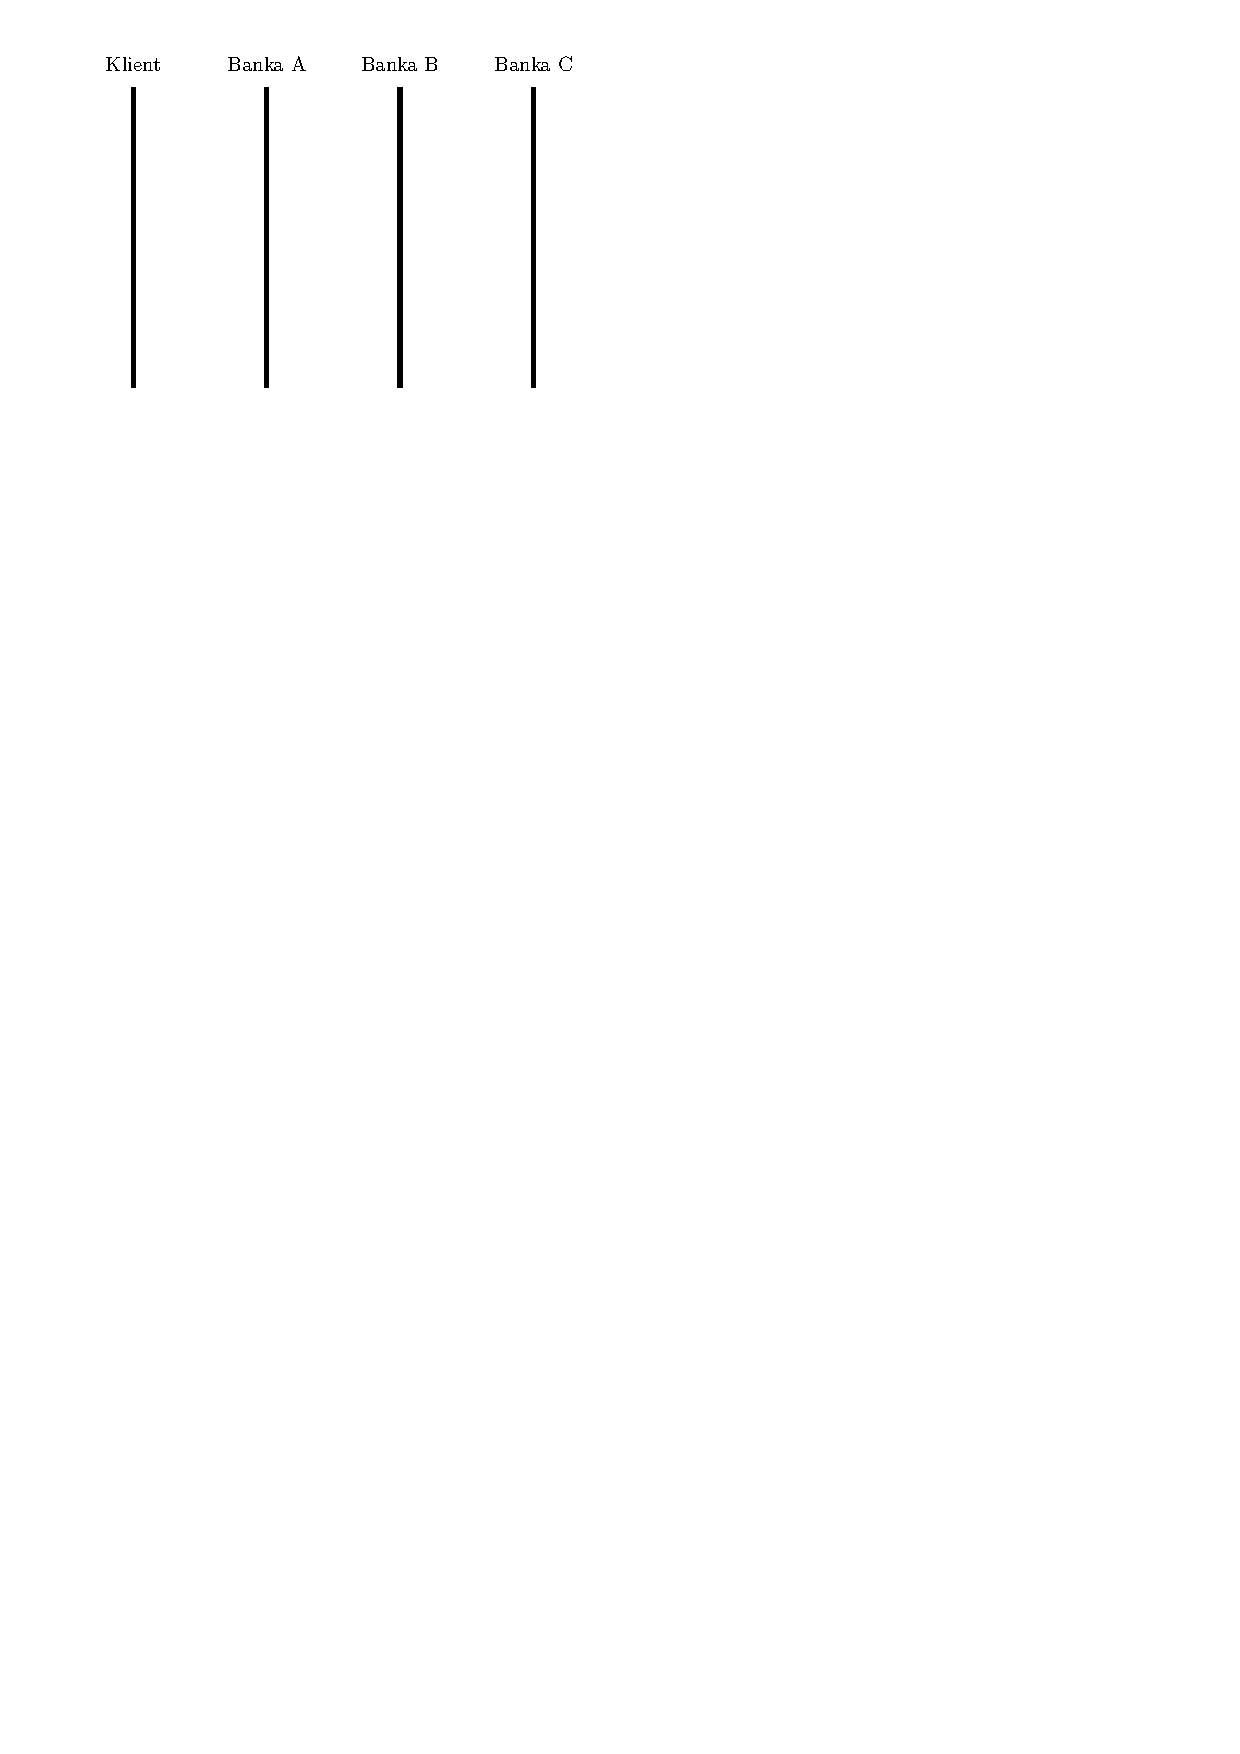
\includegraphics{10/figs/bank1.pdf}}   %
  	\only<2>{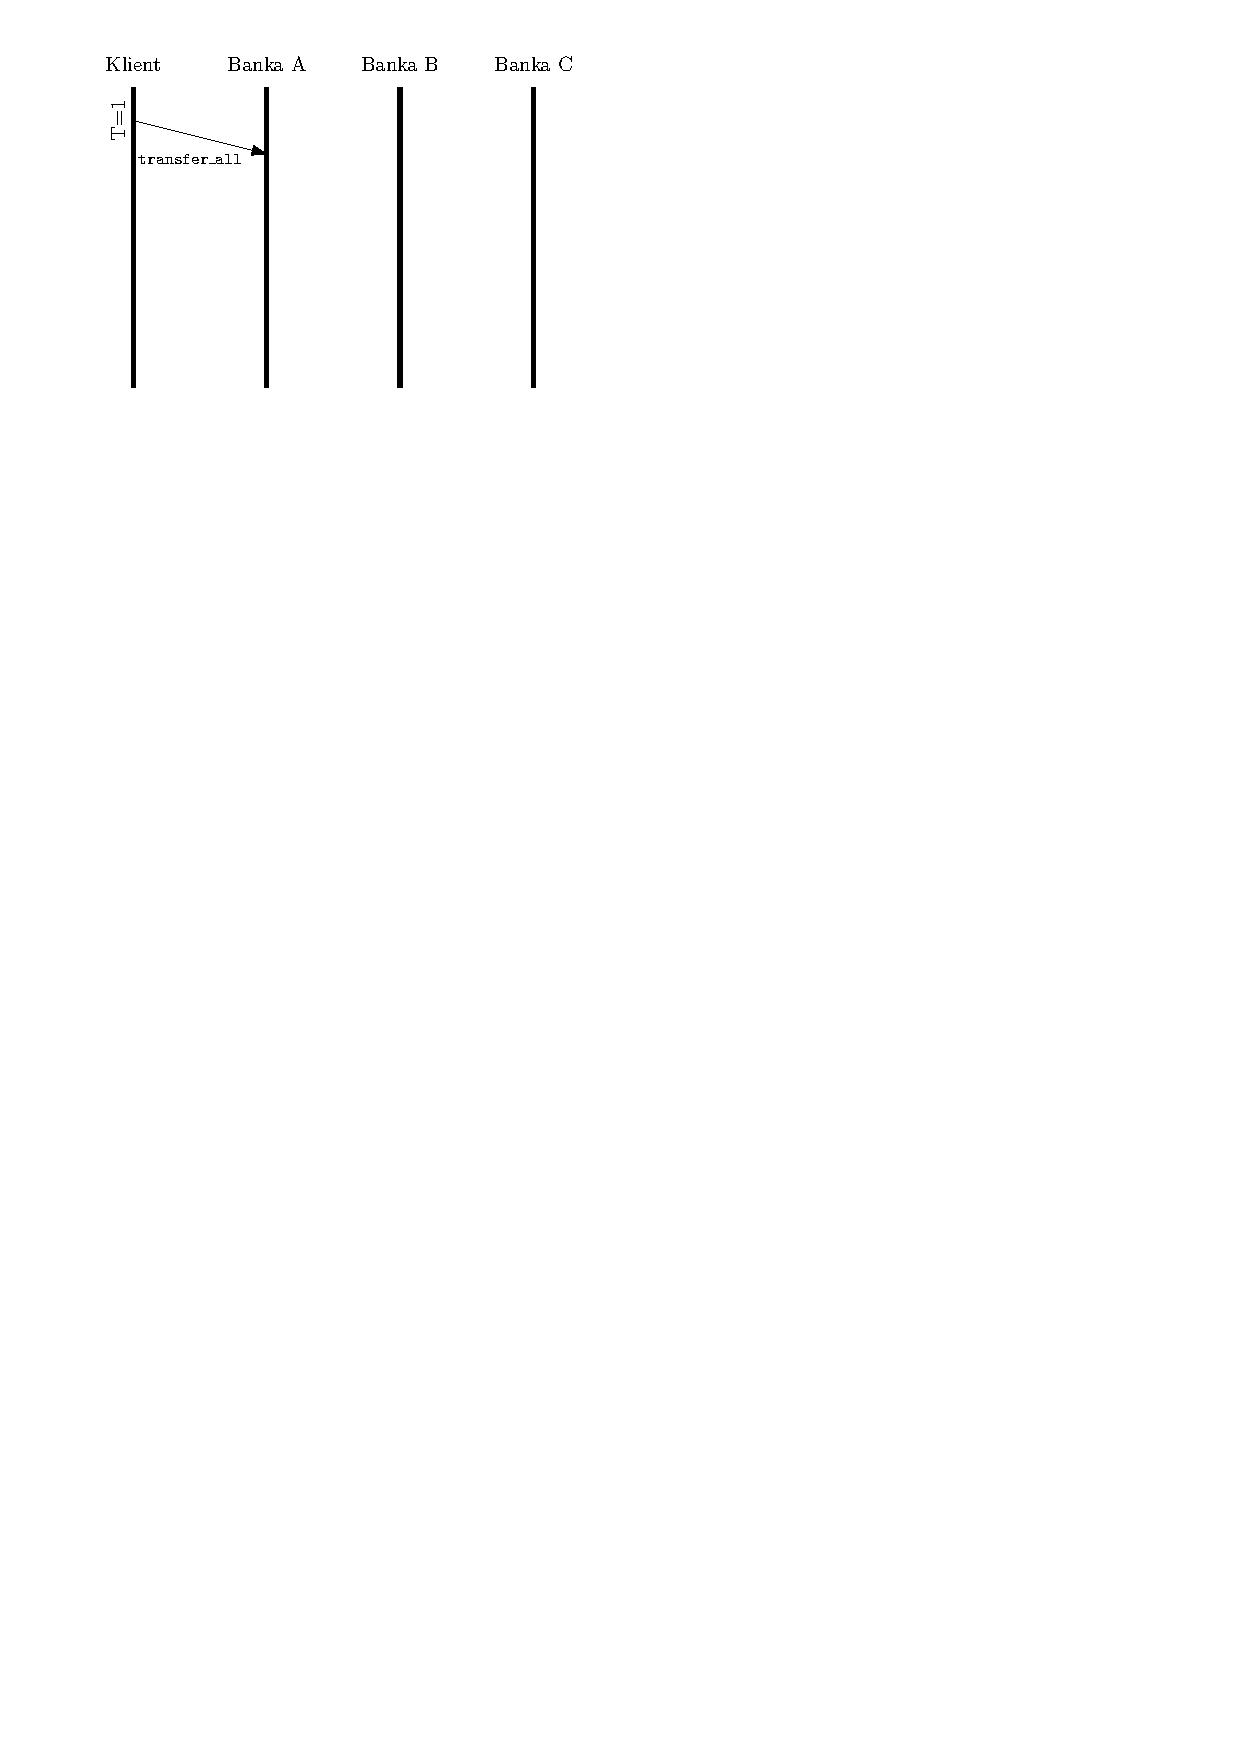
\includegraphics{10/figs/bank2.pdf}}   %
  	\only<3>{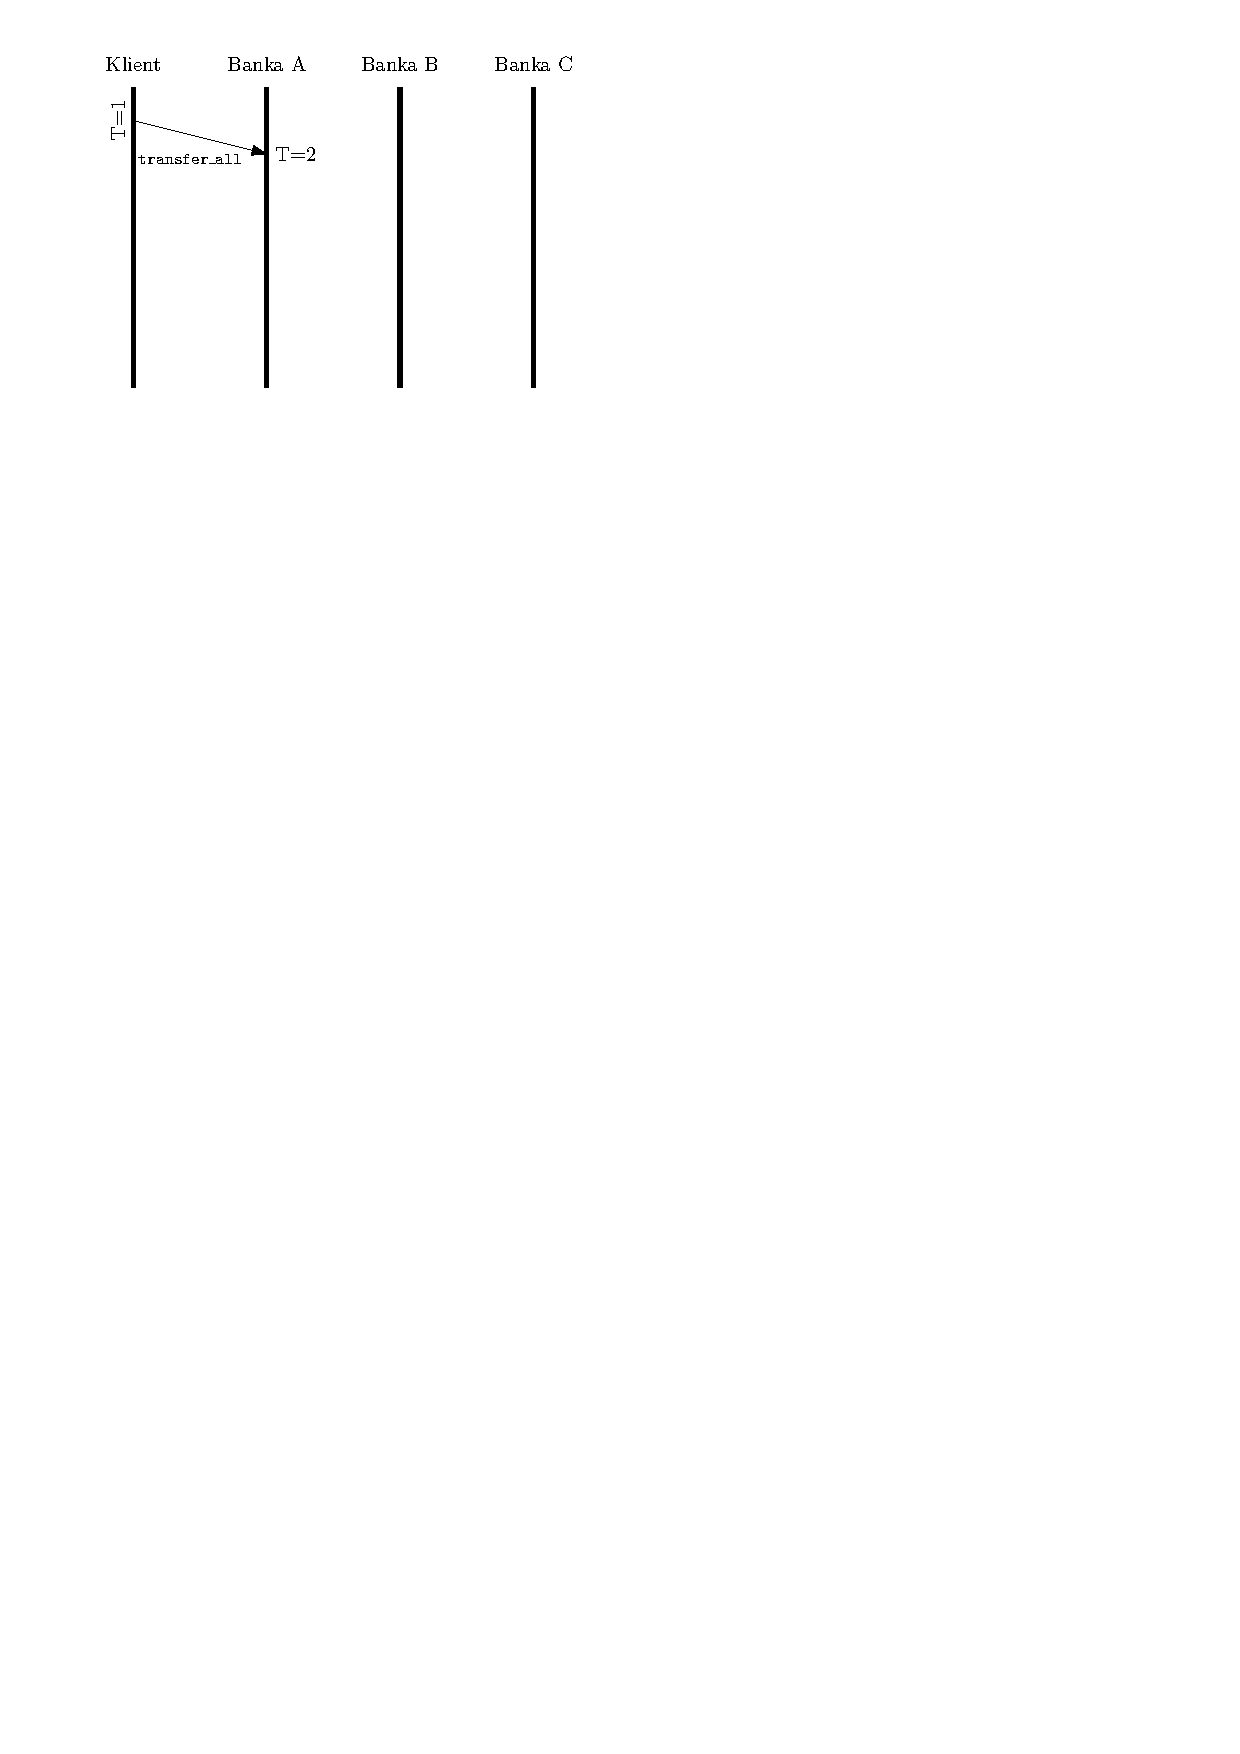
\includegraphics{10/figs/bank3.pdf}}   %
  	\only<4>{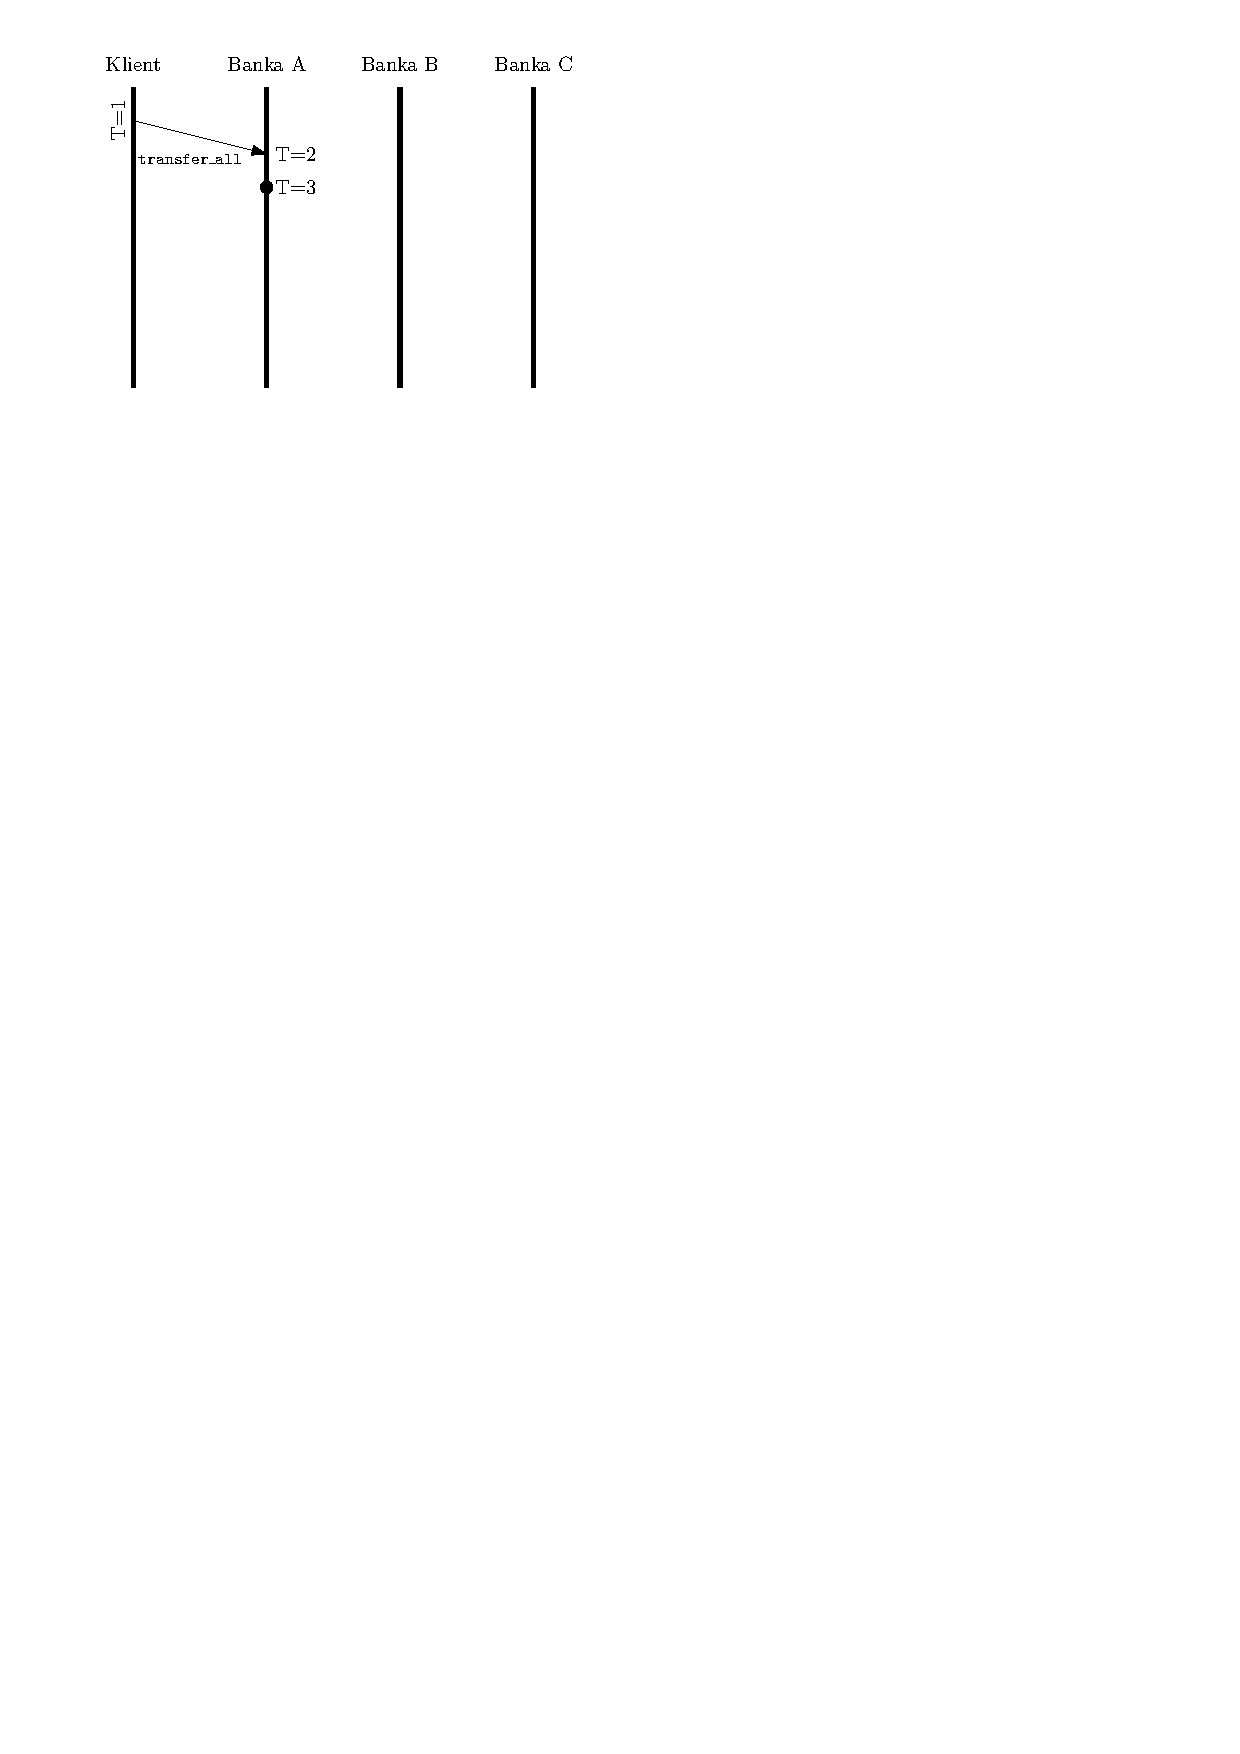
\includegraphics{10/figs/bank4.pdf}}   %
  	\only<5>{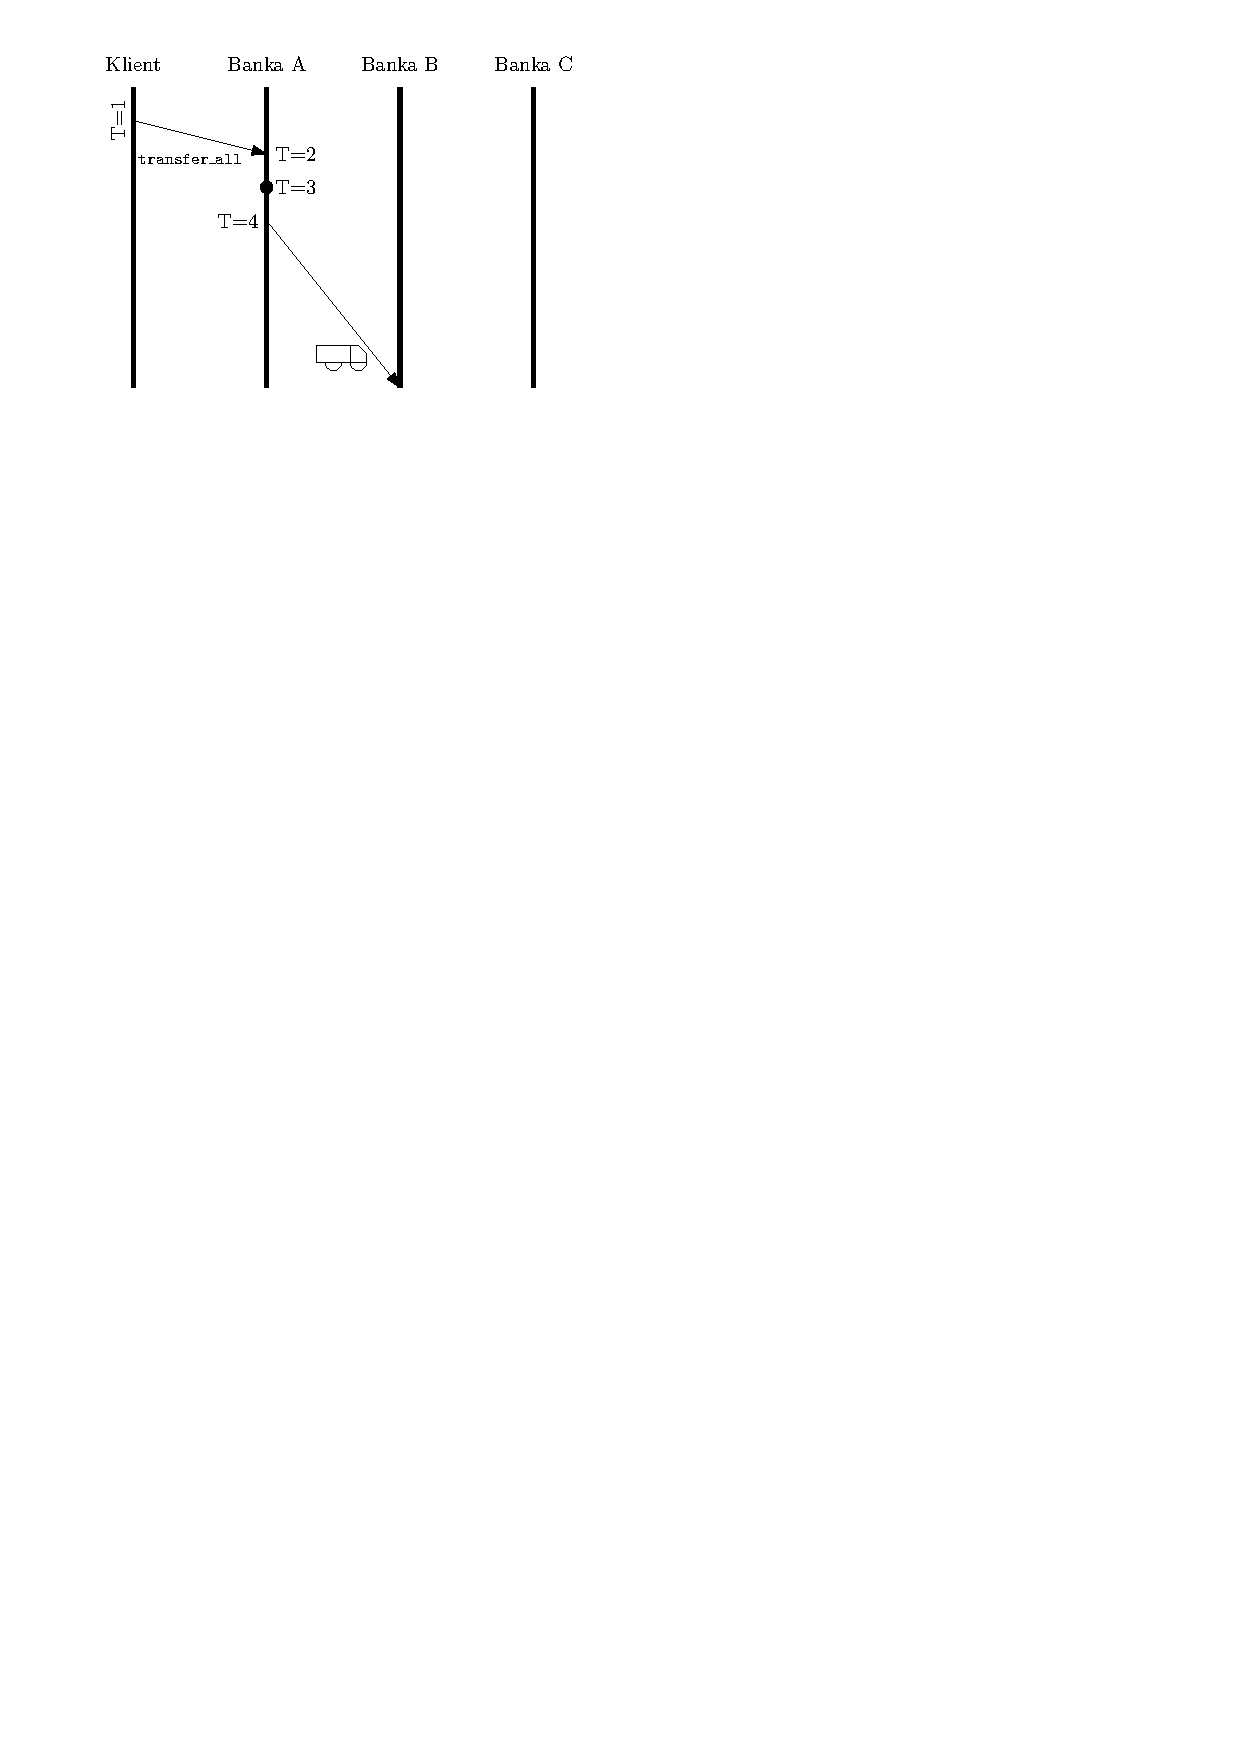
\includegraphics{10/figs/bank5.pdf}}   %
  	\only<6>{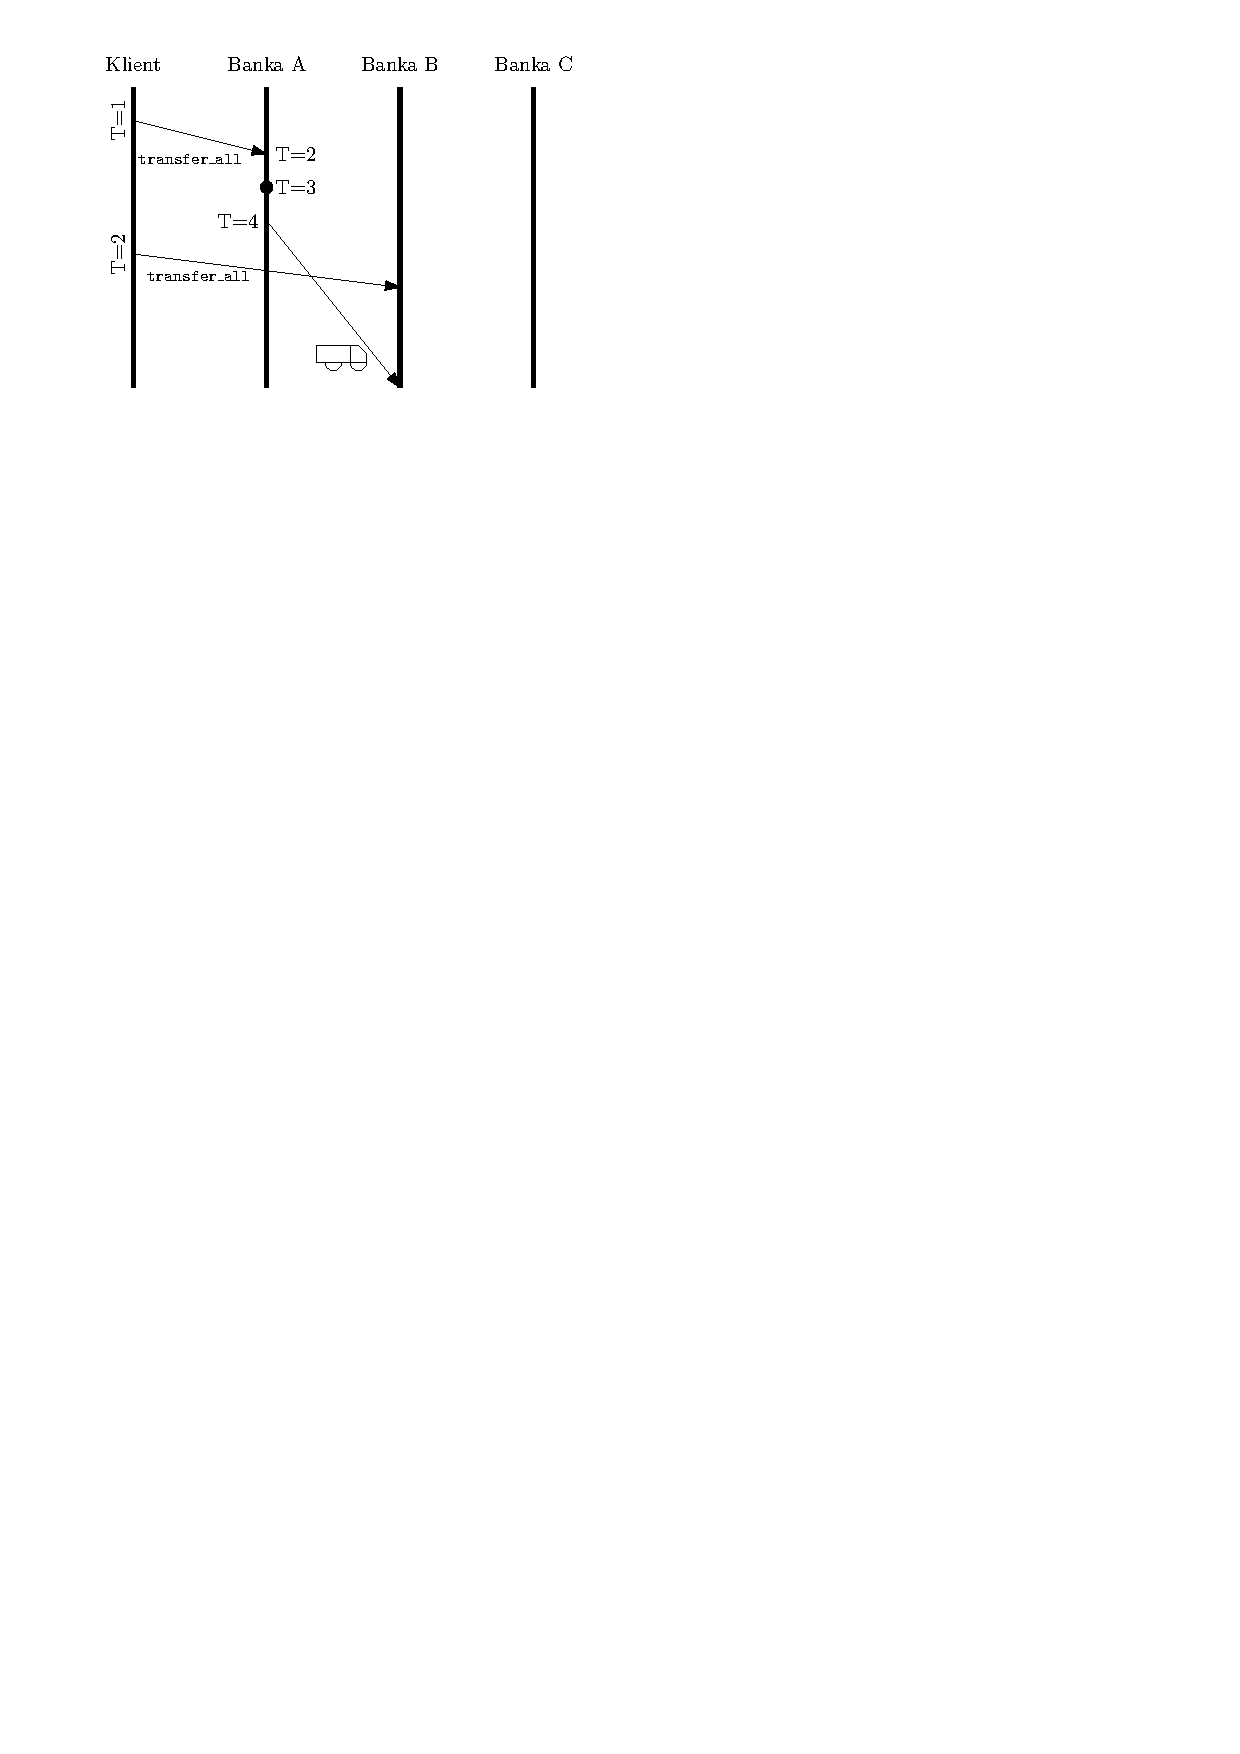
\includegraphics{10/figs/bank6.pdf}}   %
  	\only<7>{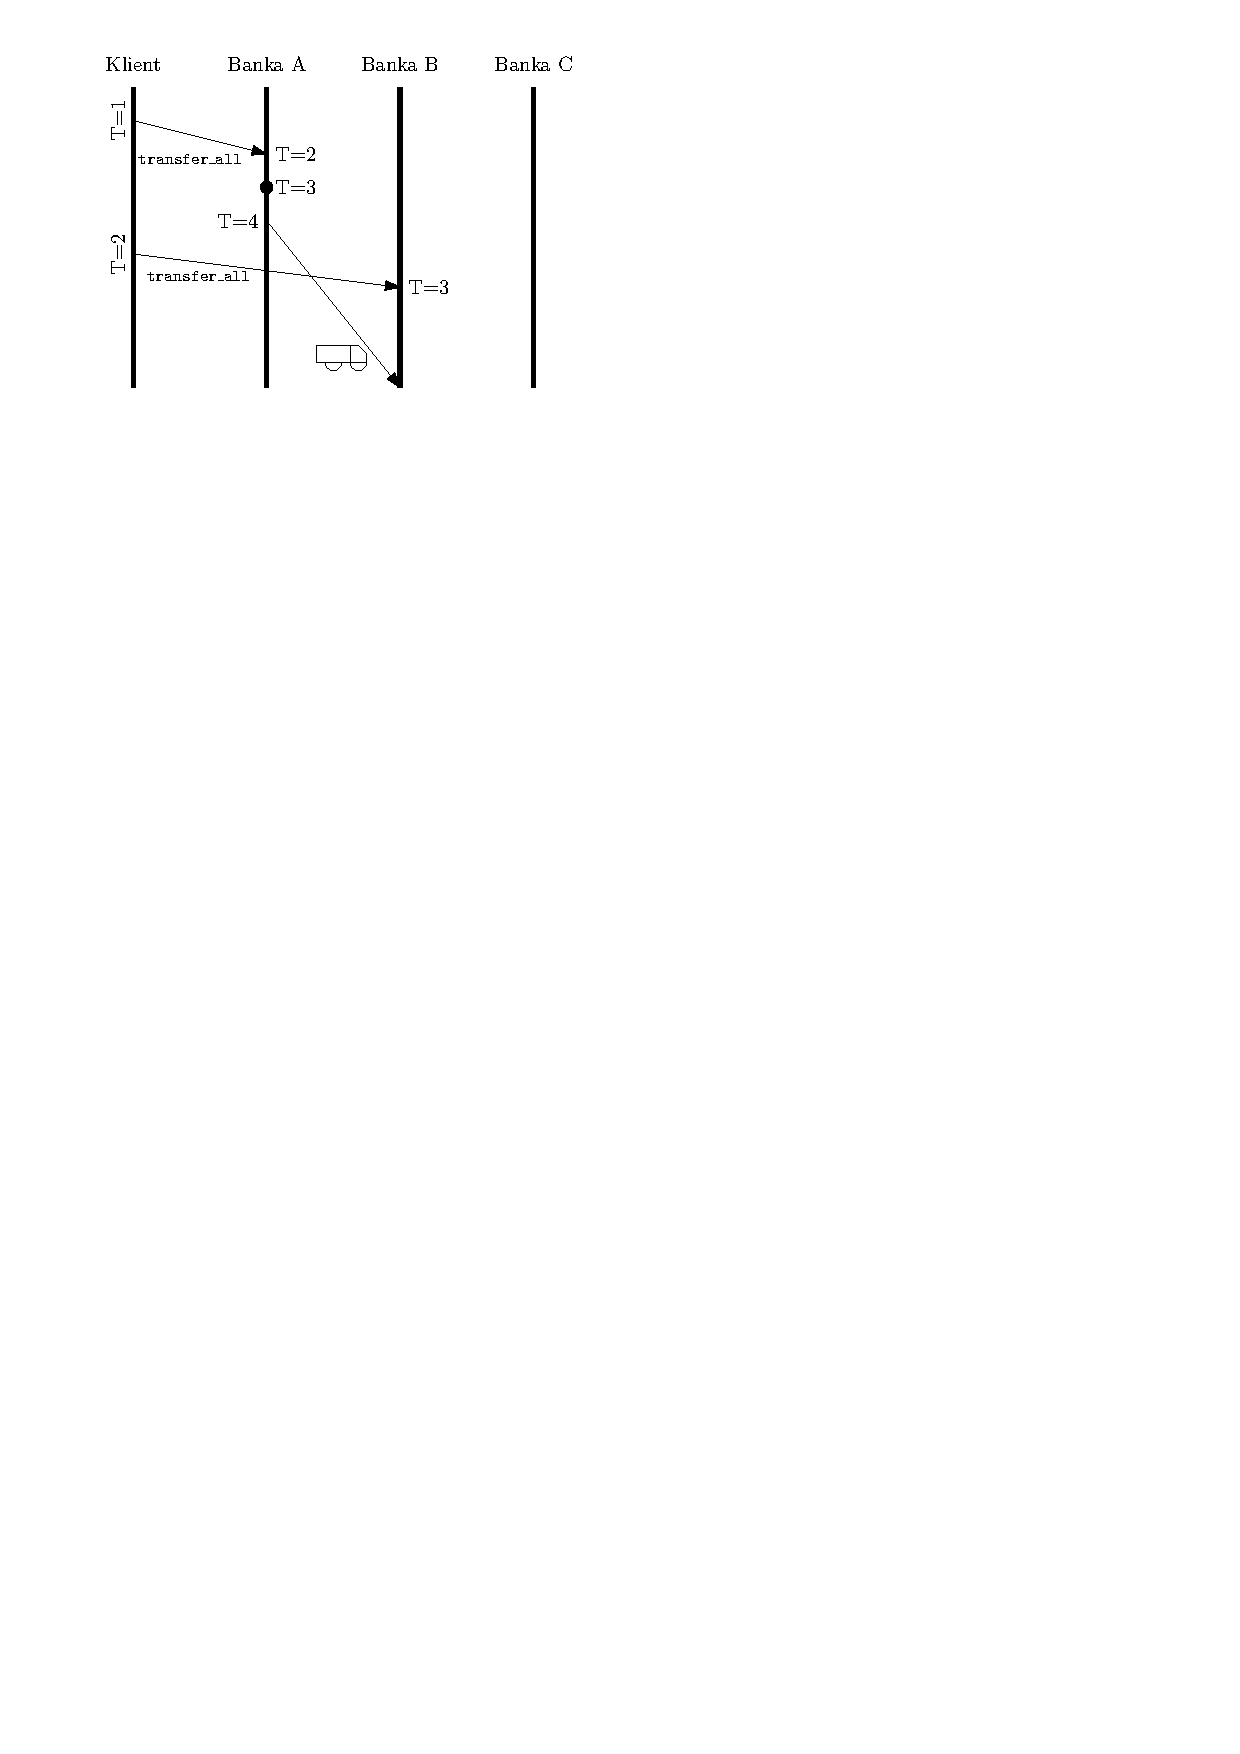
\includegraphics{10/figs/bank7.pdf}}   % 
  	\only<8>{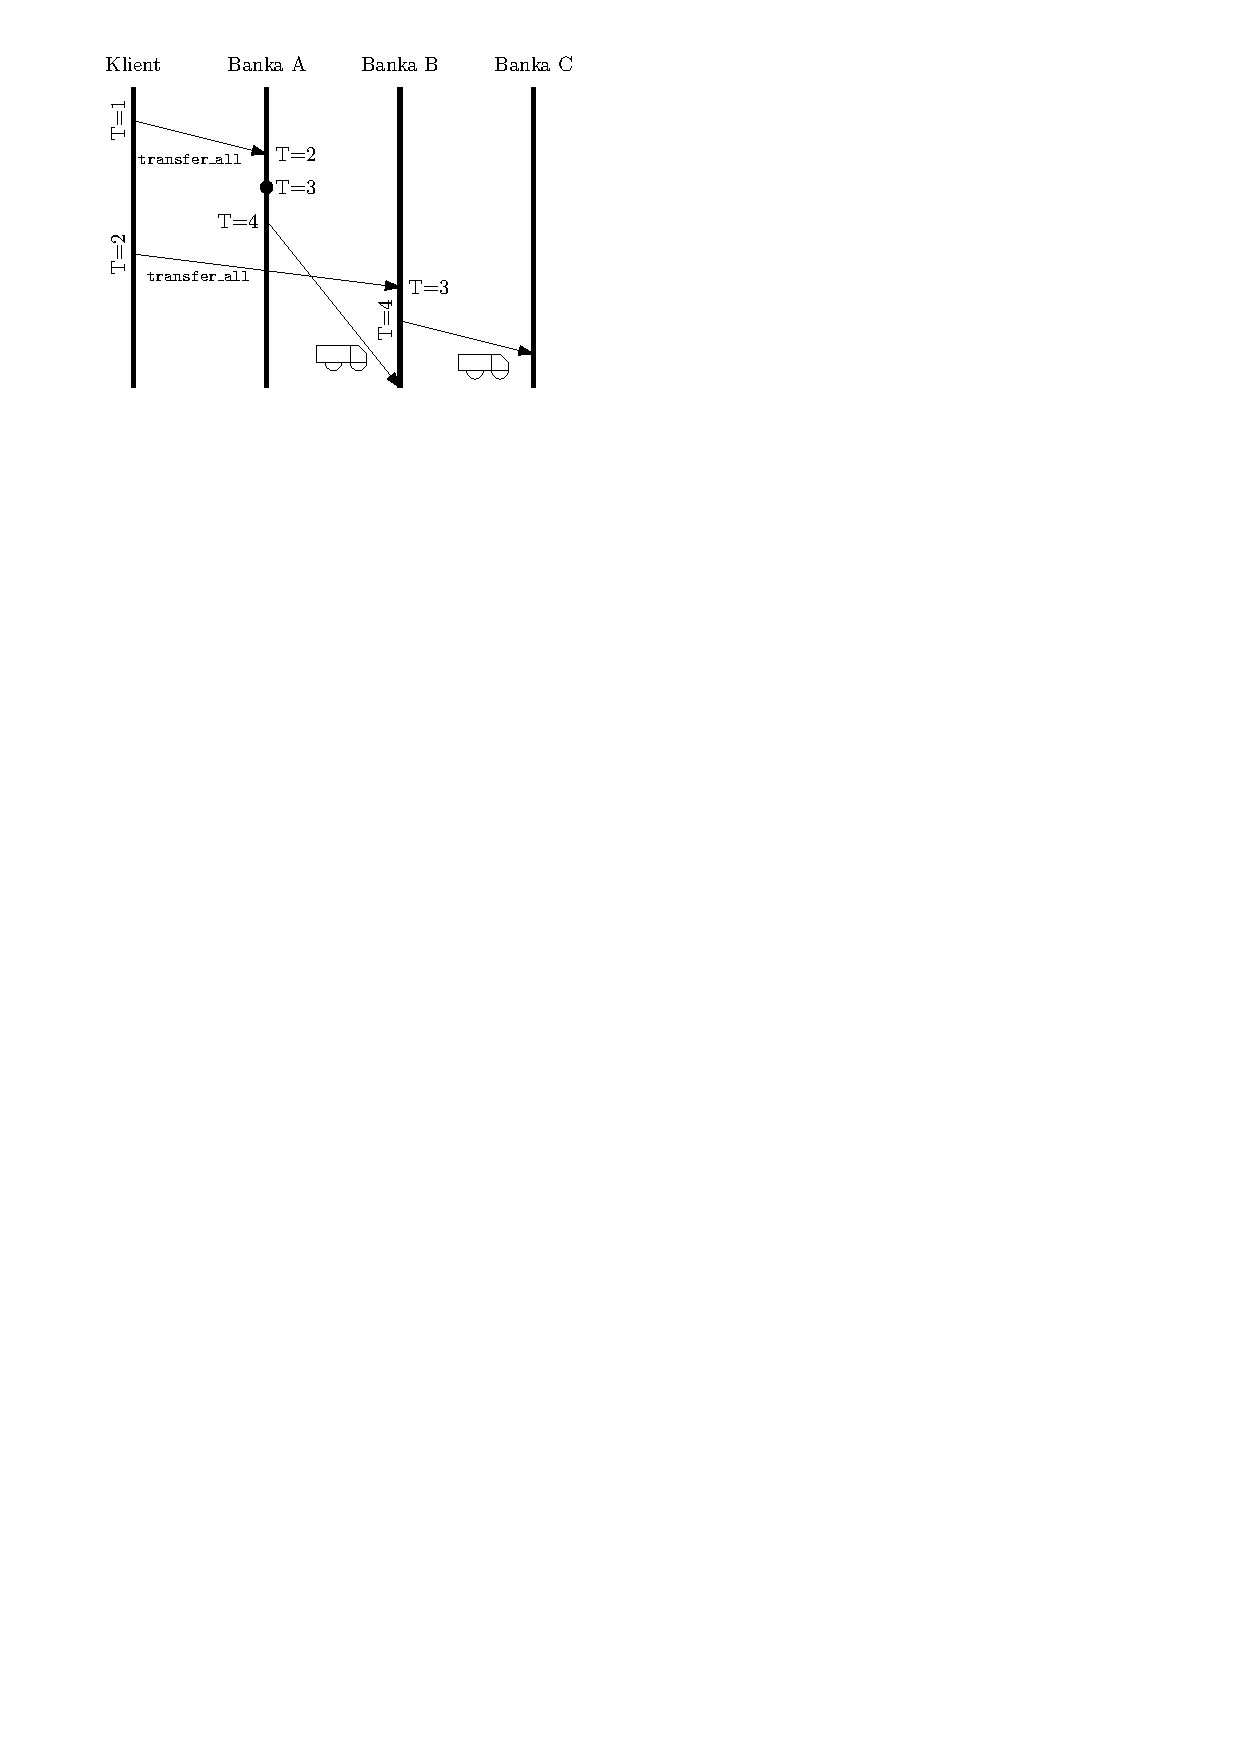
\includegraphics{10/figs/bank8.pdf}}   %
  	\only<9->{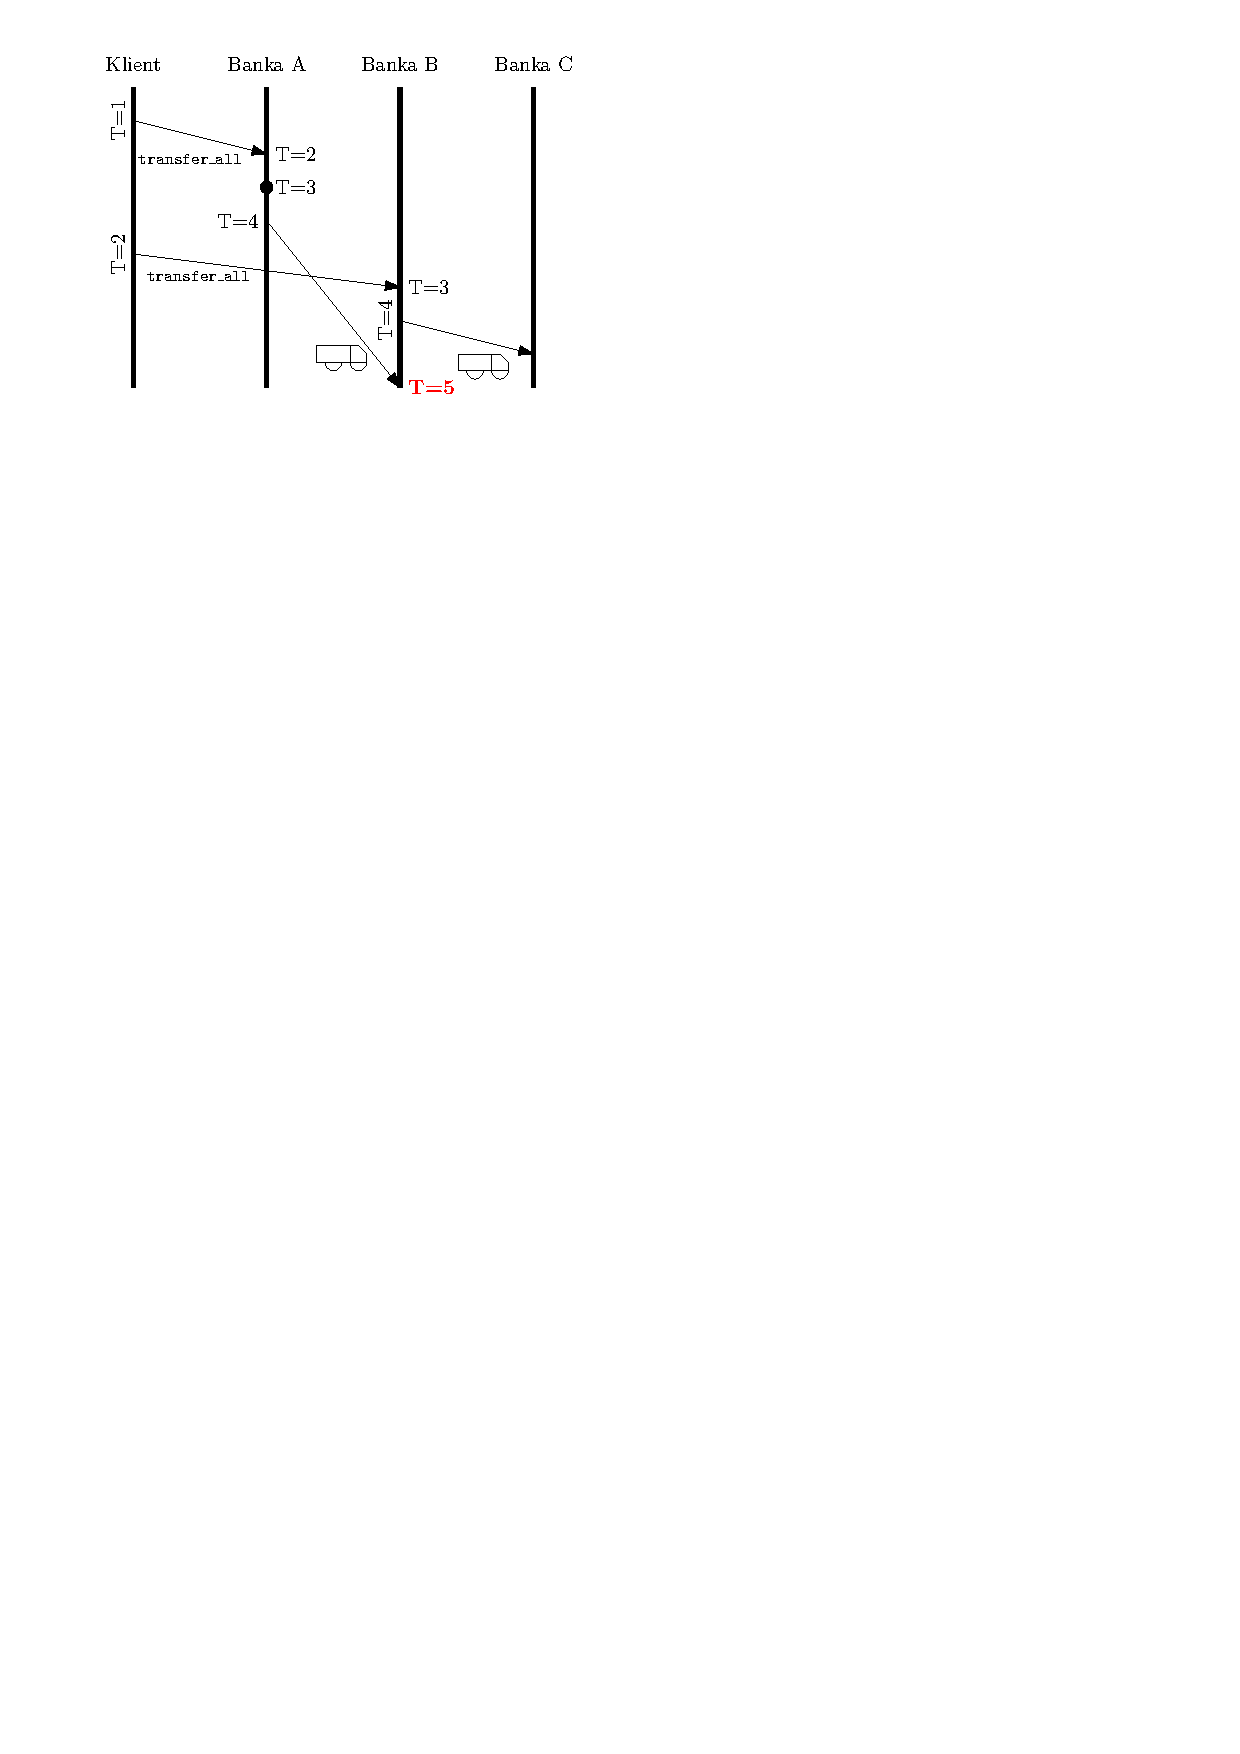
\includegraphics{10/figs/bank9.pdf}}  %
  	% Z pohledu skalarnich hodin je vse v poradku. Problem je, ze nezdetekujeme, ze je neco spatne, tzn. skalarni hodiny nepoznaji, ze prevod v T=3 prevod mel probehnout az po zprave s T=5.
  \end{center}

  \only<10>{
  	\begin{center}
  		\Large Skalární hodiny agregují všechny události do \underline{jediného} čísla :-(
  	\end{center}
  }
\end{frame}

\begin{frame}
  \frametitle{Vektorové logické hodiny}

  \begin{center}
    \LARGE \bf Vektorové hodiny
  \end{center}

  \vspace{1em}\hrule\vspace{1em}

  \begin{enumerate}
    \pause\item Místo jednoho čísla si držíme vektor časů jednotlivých agentů \\
  	            \mintinline{java}{int[] vectorTime = new int[NUM_AGENTS]}
  	\pause\item Před každou významnou událostí (obzvlášť posláním zprávy!) si proces $i$ lokální čas posune... \textbf{Ale jen svoji komponentu!} \\
  				\mintinline{java}{++vectorTime[i]}
  	\pause\item Každé zprávě přiřadíme časovou značku $\texttt{msg.}T = \texttt{vectorTime}$
  	\pause\item Po přijetí zprávy \texttt{msg} procesem $i$ si proces $i$ aktualizuje svůj \texttt{logicalTime} ve všech složkách $(\forall j)$ podle:
  				\[ \texttt{vectorTime[j]} = \begin{cases}
  				      1 + \max \lbrace \texttt{vectorTime[j]},\ \texttt{msg.}T\texttt{[j]} \rbrace & \text{if } i = j \\
  				      \max \lbrace \texttt{vectorTime[j]},\ \texttt{msg.}T\texttt{[j]} \rbrace & \text{jinak}
  				   \end{cases}
  				\]
  \end{enumerate}

  \pause
  \begin{center}
  	\bf \faWarning \hspace{3pt} Vždy posunujeme jen svoji složku časového vektoru!
  \end{center}

  %As with Lamport logical time each host maintains its own notion of the local time and updates it using the timestamps placed by the sender onto messages. But with vector logical time, the time contains more information -- it contains a vector representing the state of each host. In other words, this vector not only contains the event count for the host, itself, it also contains the last-known event counts on each and every other host.

  %Below is a summary of the rules for vector logical clocks:

  %Instead of just keeping our logical time, we keep a vector, V[], such that V[i] represents what we know of the logical time on processor i.
  %V[our_id] is our logical time
  %Send V[] vector with each message
  %On receive, merge both vectors, selecting the greater of the corresponding elements from each. Then increment the component for self. The event is said to have happened at new (incremented) time.
  %On send, increment time component for self. Send the updated timestamp vector with the message. The event is said to have happened at new (incremented) time.

\end{frame}


\begin{frame}[t]
\frametitle{PDV Cloud - připomenutí}
\vspace{2.5em}
\begin{center}
\only<1,6->{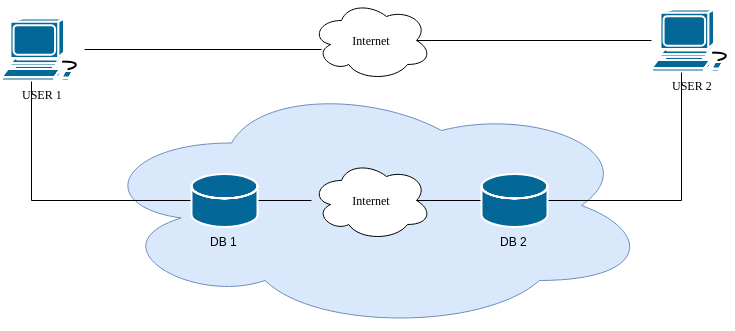
\includegraphics[scale=0.35]{10/figs/pdv_cloud.png}}%
\only<2>{\hspace{-6.4pt}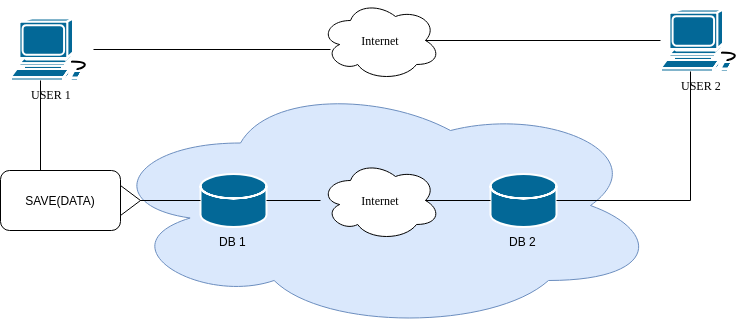
\includegraphics[scale=0.35]{10/figs/pdv_cloud_1.png}}%
\only<3>{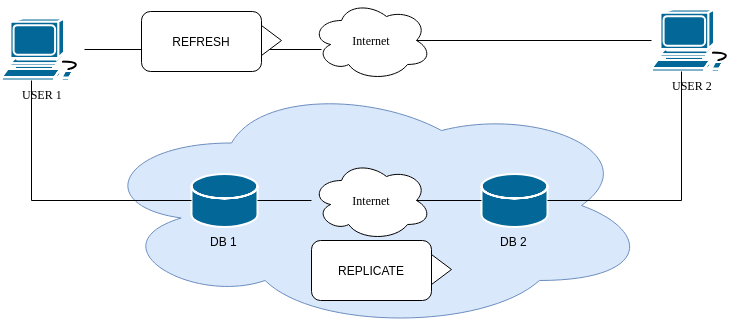
\includegraphics[scale=0.35]{10/figs/pdv_cloud_2.png}}%
\only<4>{\hspace{6.1pt}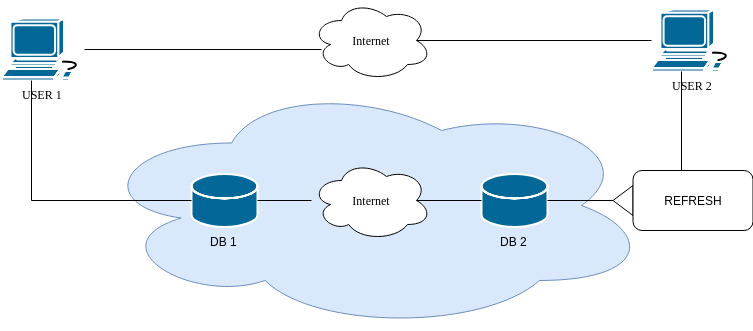
\includegraphics[scale=0.35]{10/figs/pdv_cloud_3.png}}%
\only<5>{\hspace{6.1pt}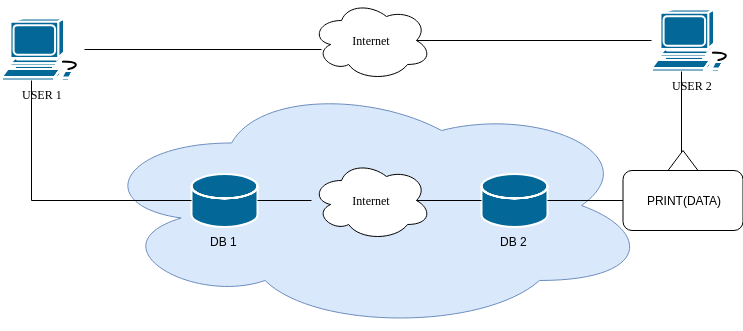
\includegraphics[scale=0.35]{10/figs/pdv_cloud_4.png}}%
\only<6>{\vspace{1em}\hrule\vspace{1em}
\ldots Doimplementujte metodu \texttt{isCausalityForProcessViolated} \hfill \\
\hfill Pak zkuste spustit scénář \texttt{ScalarDSConfigBombarding} \ldots }
\end{center}
\end{frame}


{\setbeamertemplate{frame footer}{\see{{\tt VectorClock.java} a {\tt VectorTimestamp.java}\sep{\tt Run VectorClockRun.java} v balíčku {\tt pdv\_cloud.vector}}}
\begin{frame}

  \begin{block}{Doprogramujte vektorové logické hodiny}
    Doimplementujte logiku vektorových logických hodin ve třídě \texttt{VectorClock.java}. Následně spusťte scénář \texttt{VectorClockRun.java}.
  \end{block}

  \pause\faWarning \hspace{3pt}
    \textbf{Jak využít vektorové logické hodiny k detekci souběžných událostí?}.
    % 
\end{frame}
}

\section{Vzájemné vyloučení}

\begin{frame}[fragile]

S přístupem více vláken k {\bf jednomu zdroji} jsme se již setkali

\hfill $\rightarrow$ Musíme zaručit konzistenci zdroje

\vspace{1em}

\begin{minipage}{0.4\linewidth}
Např. v {\bf OpenMp} pomocí
\end{minipage}
\begin{minipage}{0.4\linewidth}
\begin{minted}{c}
#pragma omp critical
\end{minted}
\end{minipage}

 \vspace{2em}\pause

  \begin{center}
    \LARGE Jak to vyřešit v případě DS?
  \end{center}


\end{frame}

\begin{frame}

\textit{Nejjednodušší možnost:} \large O zdroj se stará samostatný proces

\begin{itemize}
\item[$\rightarrow$] Běží na samostatném stroji
\item[$\rightarrow$] Může použít vlastní způsoby synchronizace
\end{itemize}

  \pause\vspace{1em}\hrule\vspace{1em}

  \begin{center}
    \LARGE V čem je tedy problém?
  \end{center}

\vspace{1em}\pause

Některé praktické případy DS toto {\bf neumožňují}


  \begin{itemize}
    \item Požadujeme bezstavovost zdroje \\
          {\small (souborové NFS servery)}
    \item Zdroj nemá výpočetní jednotku \\
          {\small (sítě Ethernet a IEEE 802.11, procesy přistupují k jednomu výstupnímu komunikačnímu kanálu)}
    \item ... a jiné
  \end{itemize}


\end{frame}

\begin{frame}

\frametitle{Požadavky na vzájemné vyloučení}

U procesů máme podobné požadavky jako u vláken

  \begin{itemize}
    \pause\item {\bf Safety}: v každém okamžiku ke zdroji přistupuje nanejvýš jeden proces
    \pause\item {\bf Liveness}: každá žádost o přístup ke zdroji je splněna v konečném čase
    \pause\item {\bf \textcolor{BrickRed}{Fairness}}: procesy získávají přístup k pořadí, v jakém o něj požádali
  \end{itemize}

    \vspace{1em}\hrule\vspace{1em}

    A hodnotíme je podobným způsobem

      \begin{itemize}
    \pause\item Kolik zpráv je nutné si vyměnit, aby došlo k získání a poté uvolnění zdroje?
    \pause\item Kdy nejdříve po uvolnění může zdroj získat další proces?
  \end{itemize}


\end{frame}


\begin{frame}

    \begin{center}
    \LARGE Jaké možnosti tedy v DS máme?
  \end{center}


\end{frame}

\begin{frame}
\frametitle{Centrální server}

Jeden z procesů je určený jako správce požadavků

\begin{center}
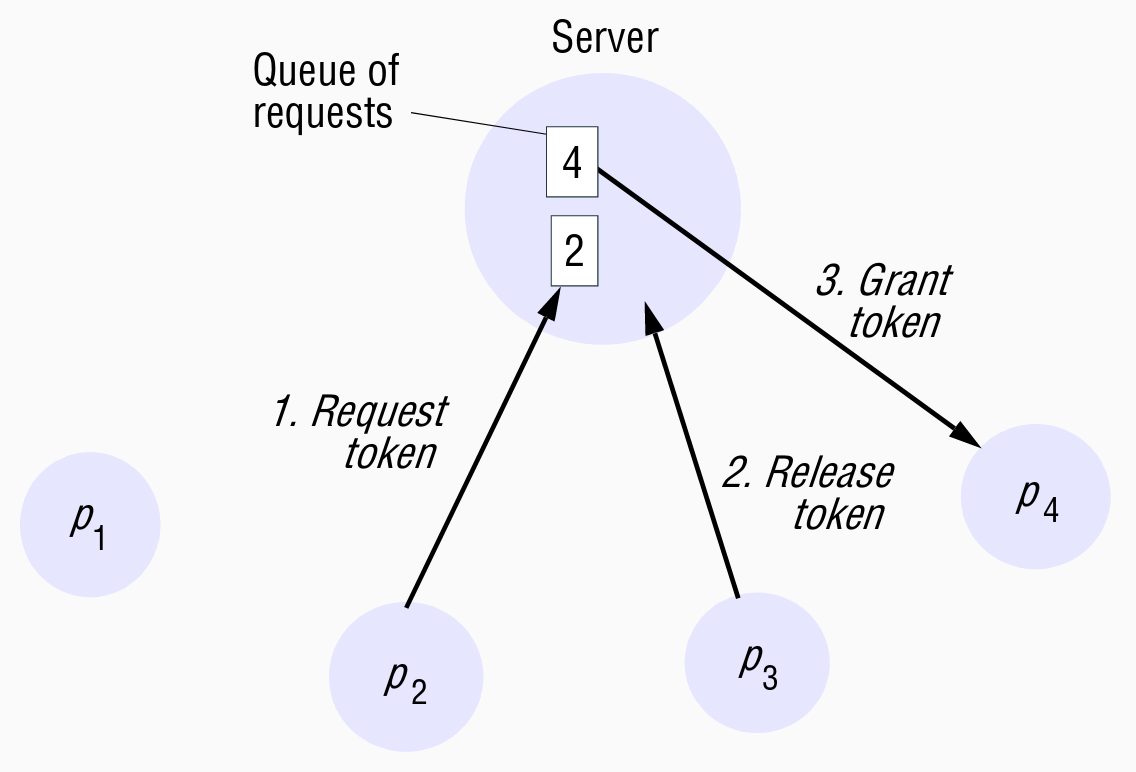
\includegraphics[width=.5\linewidth]{11/figs/central.png}
\end{center}

Udržuje si frontu doručených požadavků

Přiznává přístup ke zdroji v pořadí daném frontou

\pause\vspace{1em}

\hfill\small\bf\textcolor{BrickRed}{:(} To jsme si moc nepomohli (zavedli jsme single point of failure)

\hfill Navíc není splněn požadavek o zachování pořadí (pořadí závisí na latenci komunikace)


\end{frame}

\begin{frame}
\frametitle{Kruhové splňování}

Procesy jsou uspořádané v kruhu

\begin{center}
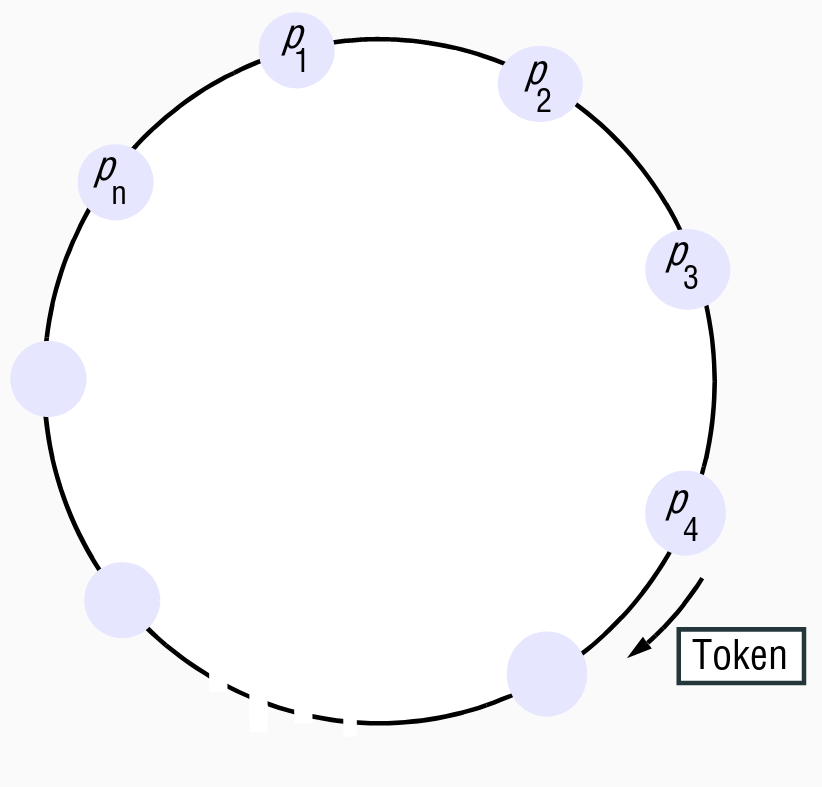
\includegraphics[width=.35\linewidth]{11/figs/circle.png}
\end{center}

Posílají si povolení k přístupu ke zdroji

Jakmile proces zdroj již nepotřebuje, pošle povolení dál

\vspace{1em}

\hfill\small\bf Opět není splněn požadavek o zachování pořadí


\end{frame}

\begin{frame}

 \begin{center}
\Large Co použít nějakou techniku kterou již známe?
\end{center}

\pause\vspace{1em}

Serializaci jsme v DS již využívali$\dots $

\pause\vspace{1em}

\hfill \bf\textcolor{BrickRed}{Hodiny!}

    \vspace{2em}\hrule\vspace{1em}

     \begin{center}
\Large Jak je tedy konkrétně použít?
\end{center}



\end{frame}

%\begin{frame}
%\frametitle{Ricart-Agrawalovo vyloučení}
% \begin{center}
%\includegraphics[width=.7\linewidth]{11/figs/ra.pdf}
%\end{center}
%\end{frame}

\begin{frame}[standout]

\vskip0pt plus 1filll %https://tex.stackexchange.com/questions/54180/how-do-i-write-something-at-the-end-of-the-slide-in-beamer

  Ricart-Agrawalovo vyloučení

% \vfill
\vskip0pt plus 1filll

% 2020: added the paper for reference
\begin{flushleft}
\tiny\see\hspace{3pt}\href{https://www.ics.uci.edu/~cs237/reading/files/Ricart and Agrawala An optimal algorithm for mutual exclusion in computer networks.pdf}
{Ricart, Agrawal: An Optimal Algorithm for Mutual Exclusion in Computer Networks, 1981}%\\[1.3em]
\end{flushleft}
\end{frame}

%
%\begin{frame}
%\frametitle{Lamportovo vyloučení}
%
%Každý proces má
%
%\begin{enumerate}
%\item lokální logické hodiny,
%\item prioritní frontu požadavků o zdroj, seřazenou podle časů požadavků, a
%\item mapu časů, kdy naposledy přijal zprávu od ostatních procesů.
%\end{enumerate}
%
%    \pause\vspace{1em}\hrule\vspace{1em}
%
%V systému kolují tři typy zpráv: {\bf REQUEST}, {\bf ACKNOWLEDGE} a {\bf RELEASE}
%
%\begin{enumerate}
%\item Pokud chce proces $P_i$ požádat o zdroj, zaznamená čas $T_A$ kdy o zdroj žádá a pošle zprávu REQUEST s tímto časem všem procesům. Přidá $\{P_i : T_A\}$ do prioritní fronty.
%\item Pokud procesu $P_j$ přijde zpráva REQUEST od procesu $P_i$, přidá $\{P_i : T_A\}$ do prioritní fronty, a odpoví $P_i$ zprávou ACKNOWLEDGE.
%\item Pokud procesu $P_i$ přijde zpráva ACKNOWLEDGE od procesu $P_j$, provede update času naposledy doručené zprávy od $P_j$.
%\end{enumerate}
%
%\end{frame}
%
%
%\begin{frame}
%\frametitle{Lamportovo vyloučení}
%
%\begin{enumerate}
%\setcounter{enumi}{3}
%\item Pokud chce proces $P_i$ uvolnit zdroj, vyjme své požadavky z prioritní fronty a pošle zprávu RELEASE všem procesům.
%\item Pokud procesu $P_j$ přijde zpráva RELEASE od procesu $P_i$, vyjme všechny požadavky procesu $P_i$ z prioritní fronty.
%\end{enumerate}
%
%    \pause\vspace{1em}\hrule\vspace{1em}
%
%     \begin{center}
%\Large Kdy ted proces zdroj získá?
%\end{center}
%\pause
%Musí být splněny dva požadavky
%
%\begin{enumerate}
%\item[(i)] Požadavek musí být na vrcholu fronty, a
%\item[(ii)] časy naposledy doručených zpráv ostatních procesů musí být větší než čas požadavku.
%\end{enumerate}
%\end{frame}


% \begin{frame}
% \frametitle{Ricart-Agrawalovo vyloučení}

% Každý proces má své lokální skalární logické hodiny, a zámek (či několik zámků), kde každý má
% \begin{enumerate}
% \item identifikátor kritické sekce, kterou zamyká,
% \item stav: {\bf RELEASED}, {\bf HELD} nebo {\bf WANTED}, a
% \item frontu odložených požadavků.
%   \end{enumerate}

% V systému kolují pro každou kritickou sekci dva typy zpráv:  {\bf REQUEST} a {\bf OK}
% \begin{enumerate}
% \item Pokud chce proces $P_i$ požádat o vstup do kritické sekce K, zaznamená čas $T_i$ kdy o zdroj žádá a pošle zprávu REQUEST(K) s tímto časem všem procesům, které do K přistupují. Nastaví stav zámku na {\bf WANTED}.
% \item Zámek K procesu je ve stavu  {\bf WANTED} dokud neobdrží zprávu OK(K) od každého dalšího přistupujícího procesu. Poté se nastaví na  {\bf HELD}.
% \item Pokud procesu $P_i$ přijde zpráva REQUEST(K) od procesu $P_j$ s časem $T_j$:
% \begin{enumerate}
% \item[(i)] pokud je zámek K ve stavu  {\bf RELEASED}, nebo je ve stavu {\bf WANTED} a o vstup do kritické sekce žádal v čase $T_i > T_j$, pak pošle zprávu OK(K) procesu $P_j$,
% \item[(ii)] jinak požadavek odloží a neodpoví.
% \end{enumerate}
% \item Pokud proces $P_i$ dokončí práci v kritické sekci K, nastaví stav zámku K na {\bf RELEASED}, odpoví na všechny odložené požadavky a frontu požadavků vyprázdní.
% \end{enumerate}

% %Každý proces má
% %
% %\begin{enumerate}
% %\item lokální logické hodiny,
% %\item lokání stav: {\bf RELEASED}, {\bf HELD} nebo {\bf WANTED}, a
% %\item frontu uložených zpráv.
% %\end{enumerate}
% %
% %    \pause\vspace{1em}\hrule\vspace{1em}
% %
% %V systému kolují dva typy zpráv: {\bf REQUEST} a {\bf ACKNOWLEDGE}
% %
% %\begin{enumerate}
% %\item Pokud chce proces $P_i$ požádat o zdroj, zaznamená čas $T_i$ kdy o zdroj žádá a pošle zprávu REQUEST s tímto časem všem procesům. Nastaví svůj stav na {\bf WANTED}.
% %\item Proces je ve stavu  {\bf WANTED} dokud neobdrží zprávu ACKNOWLEDGE od každého dalšího procesu. Poté se nastaví na {\bf HELD}.
% %\item Pokud procesu $P_j$ přijde zpráva REQUEST od procesu $P_i$ s časem $T_i$, tak
% %\begin{enumerate}
% %\item[i.] pokud je ve stavu {\bf HELD}, nebo je ve stavu {\bf WANTED} a o zdroj žádal v čase $T_j < T_i$, pak REQUEST zprávu zařadí do fronty zpráv a neodpoví,
% %\item[ii.] jinak pošle zprávu ACKNOWLEDGE procesu $P_i$.
% %\end{enumerate}
% %\item Pokud proces $P_i$ dokončí práci se zdrojem, nastaví svůj stav na {\bf RELEASED}, odpoví na všechny zprávy ve frontě a frontu vyprázdní.
% %\end{enumerate}

% \end{frame}

% \section{Žádost o vstup do kritické sekce}

\begin{frame}[t]
	\frametitle{Žádost o vstup do kritické sekce}
	\vspace{1.8em}
	\begin{center}
		\only<1>{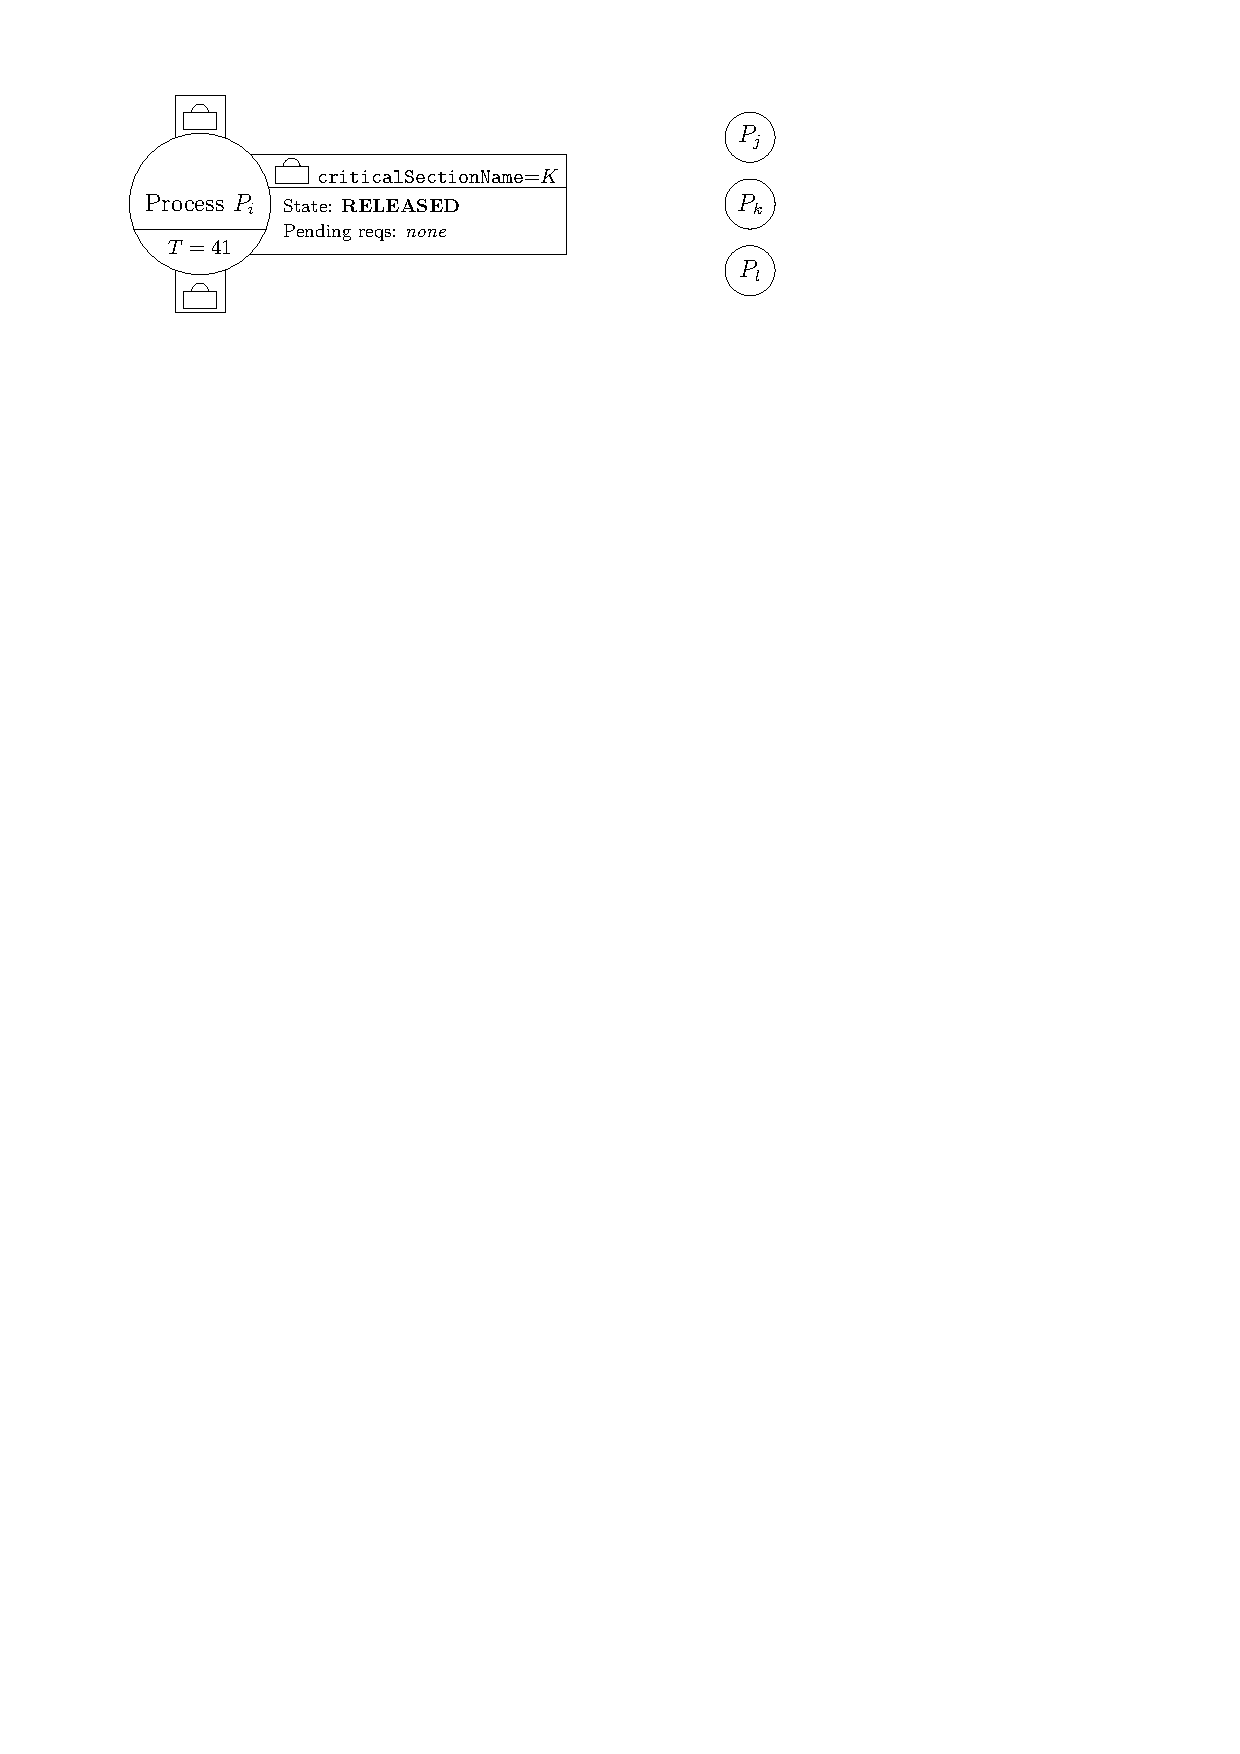
\includegraphics[width=0.95\linewidth]{11/figs/mutex_base.pdf}}%
		\only<2>{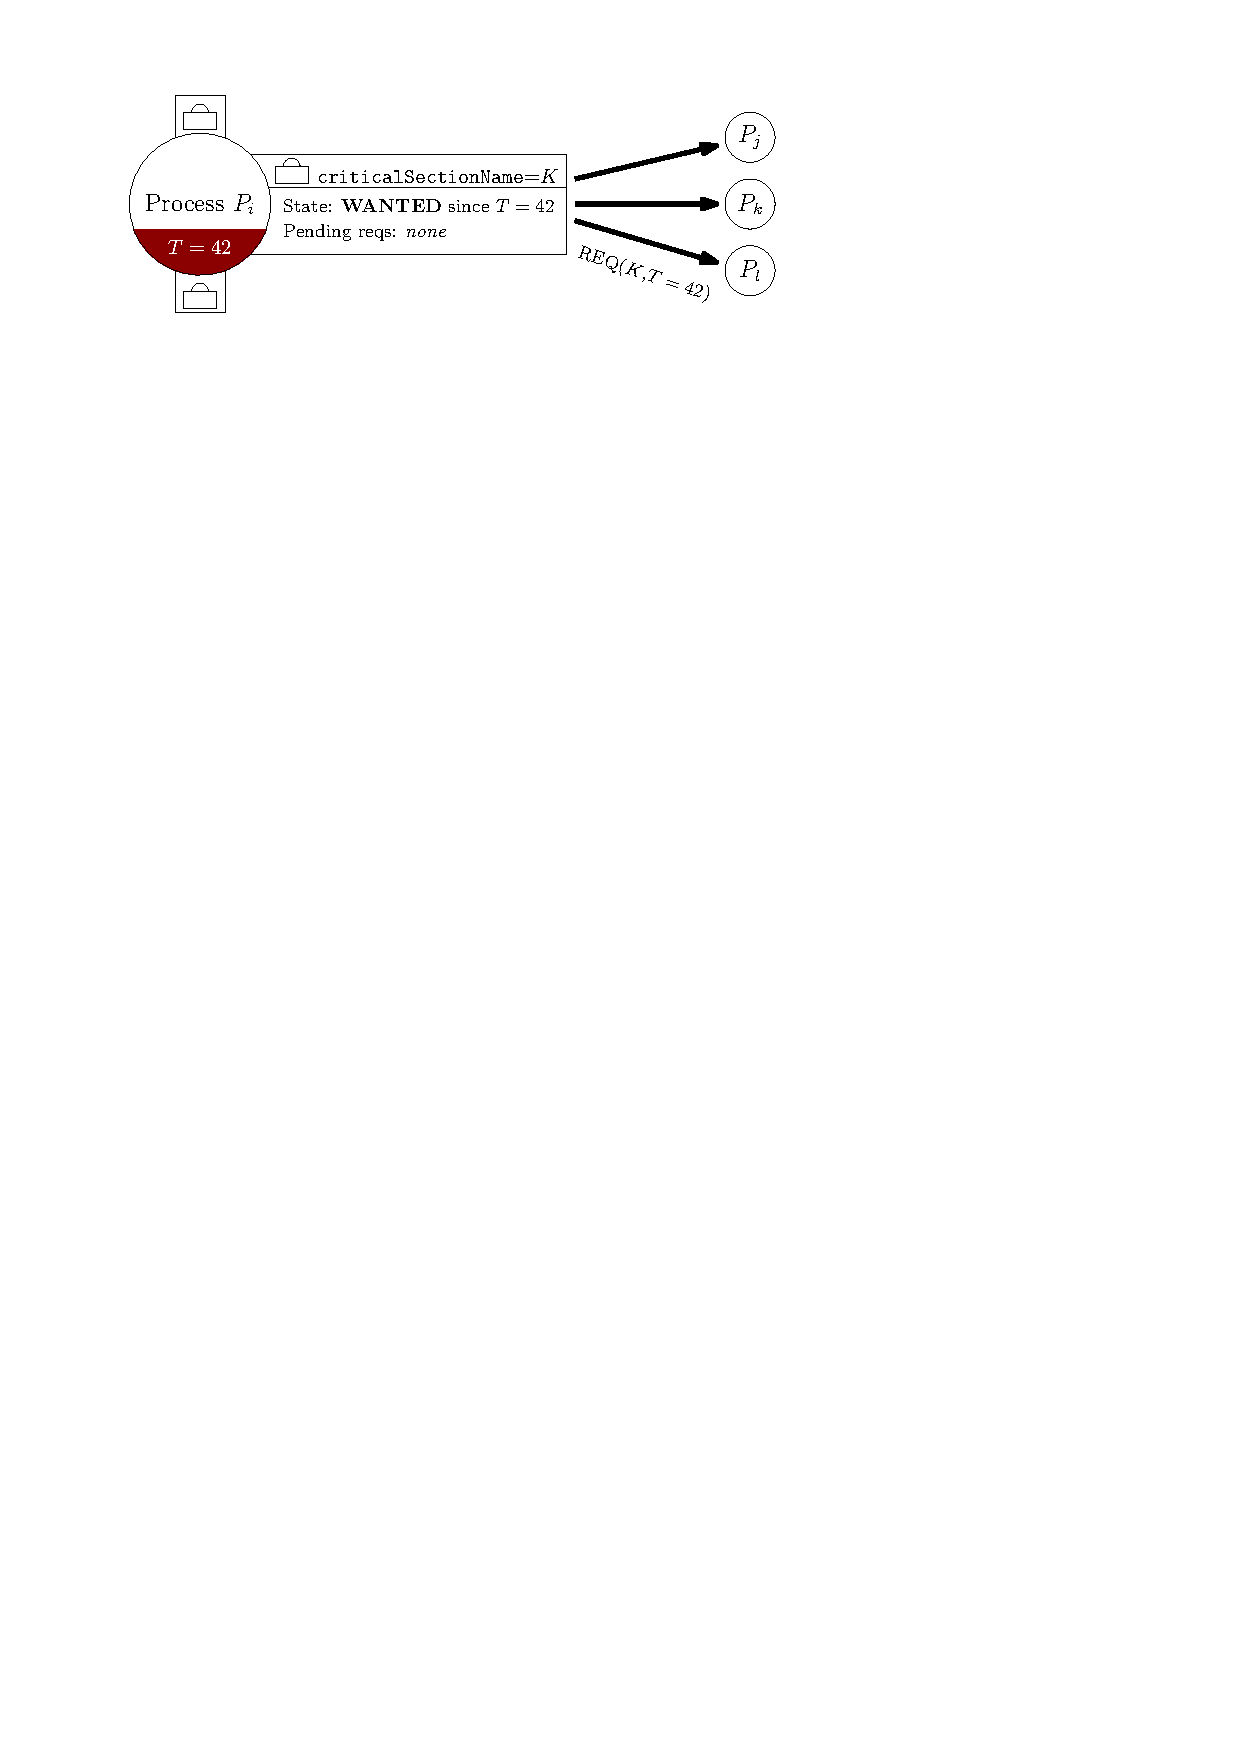
\includegraphics[width=0.95\linewidth]{11/figs/mutex_req.pdf}}%
	\end{center}

	\only<2>{
		\vspace{2em}\hrule\vspace{1em}
		\begin{enumerate}
			\item Pokud chce proces $P_i$ požádat o vstup do kritické sekce K, zaznamená čas $T_i$ kdy o zdroj žádá a pošle zprávu REQUEST(K) s tímto časem všem procesům, které do K přistupují. Nastaví stav zámku na {\bf WANTED}.
		\end{enumerate}
	}
\end{frame}

\begin{frame}[t]
	\frametitle{Žádost o vstup do kritické sekce}
	\vspace{1.8em}
	\begin{center}
		\only<1>{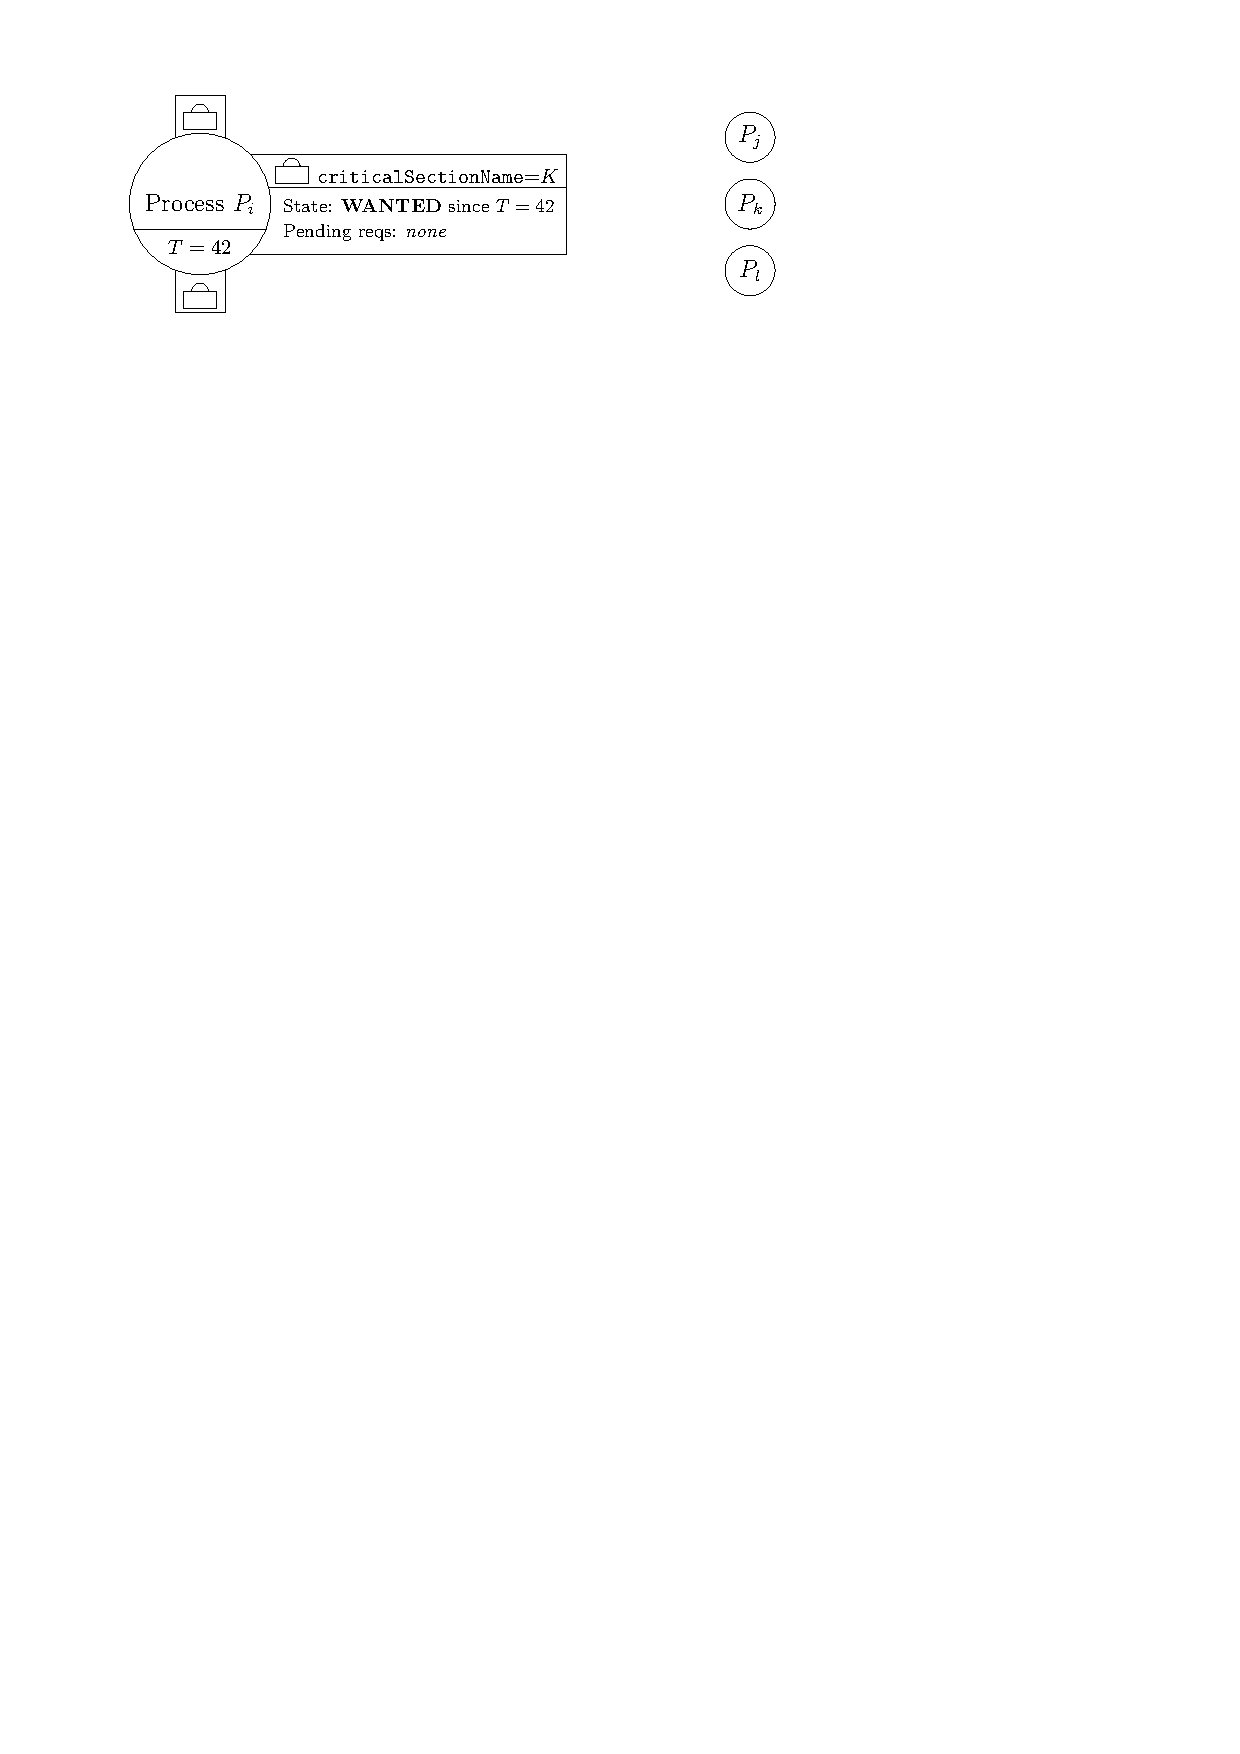
\includegraphics[width=0.95\linewidth]{11/figs/mutex_ok_1.pdf}}%
		\only<2>{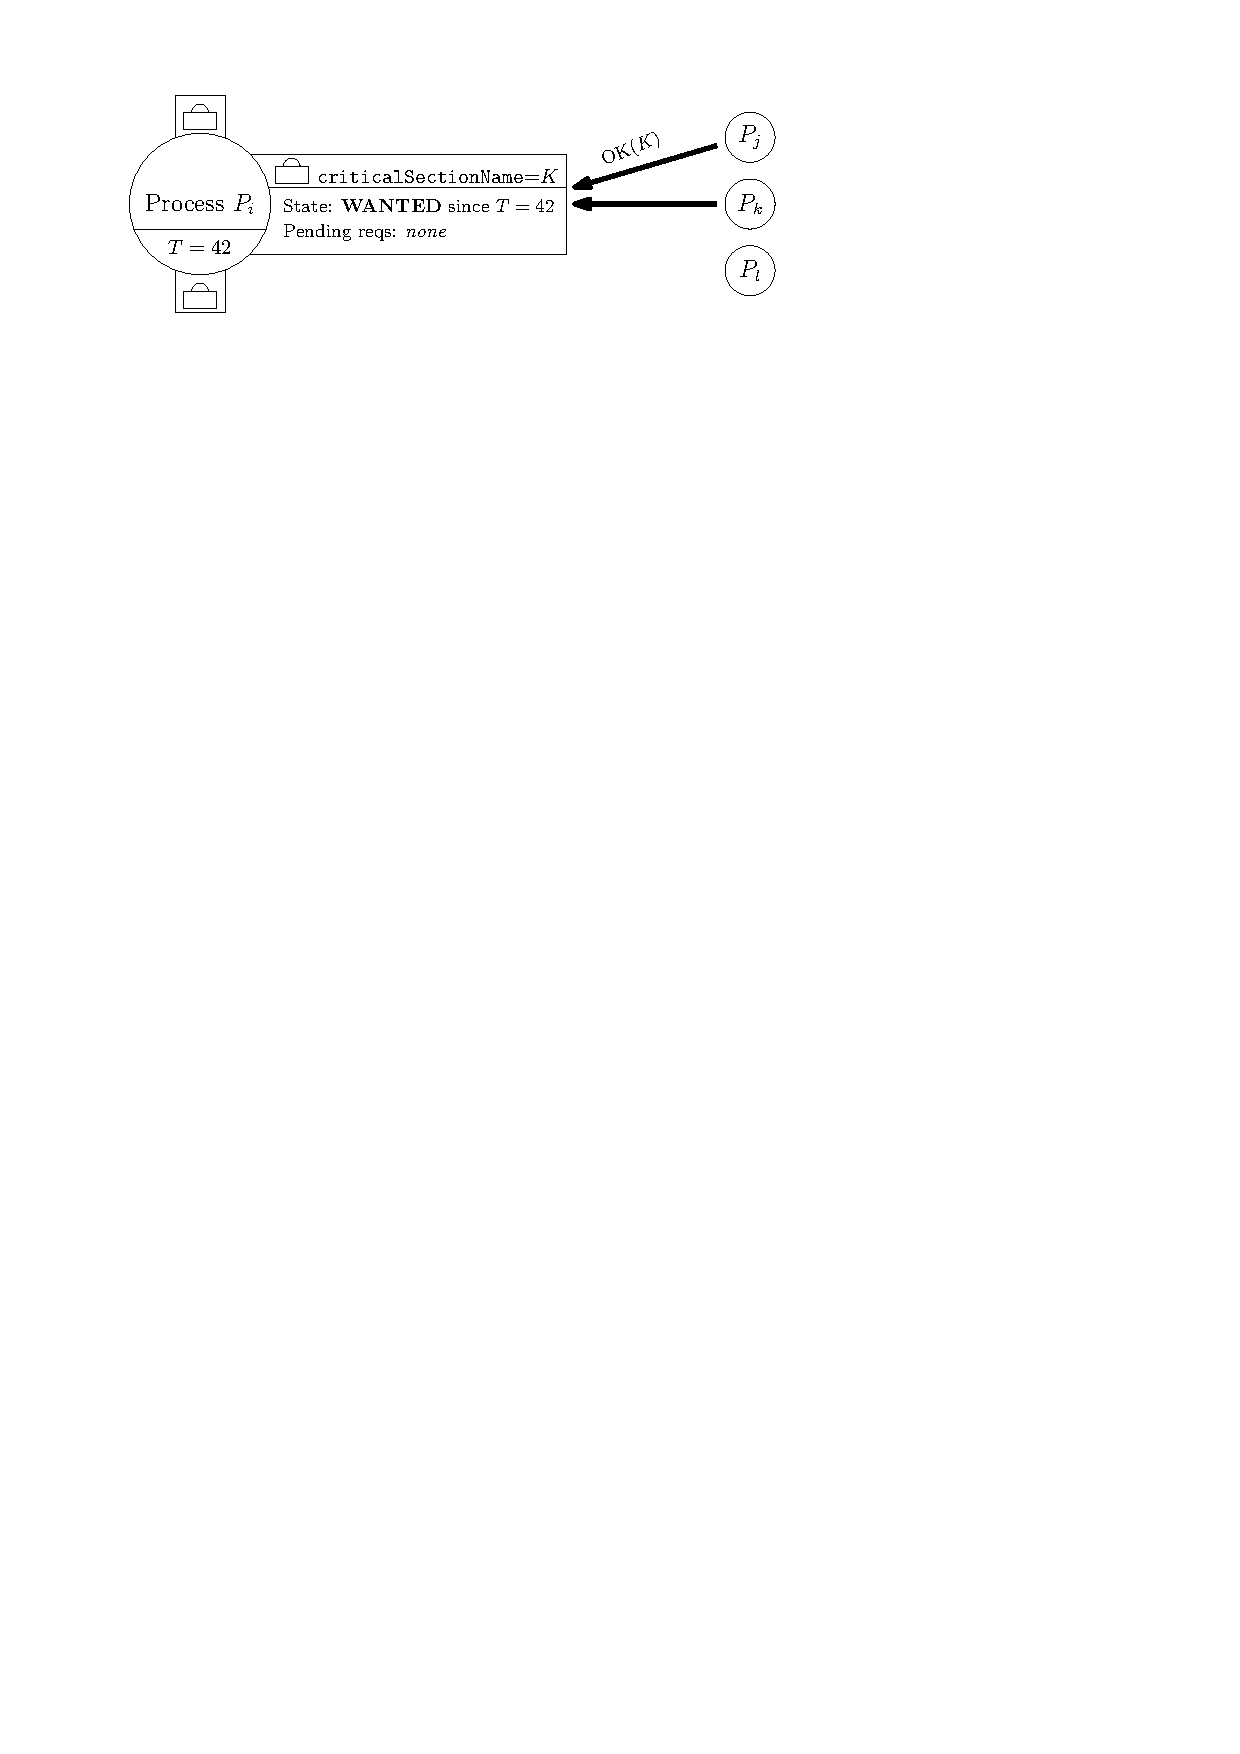
\includegraphics[width=0.95\linewidth]{11/figs/mutex_ok_2.pdf}}%
		\only<3>{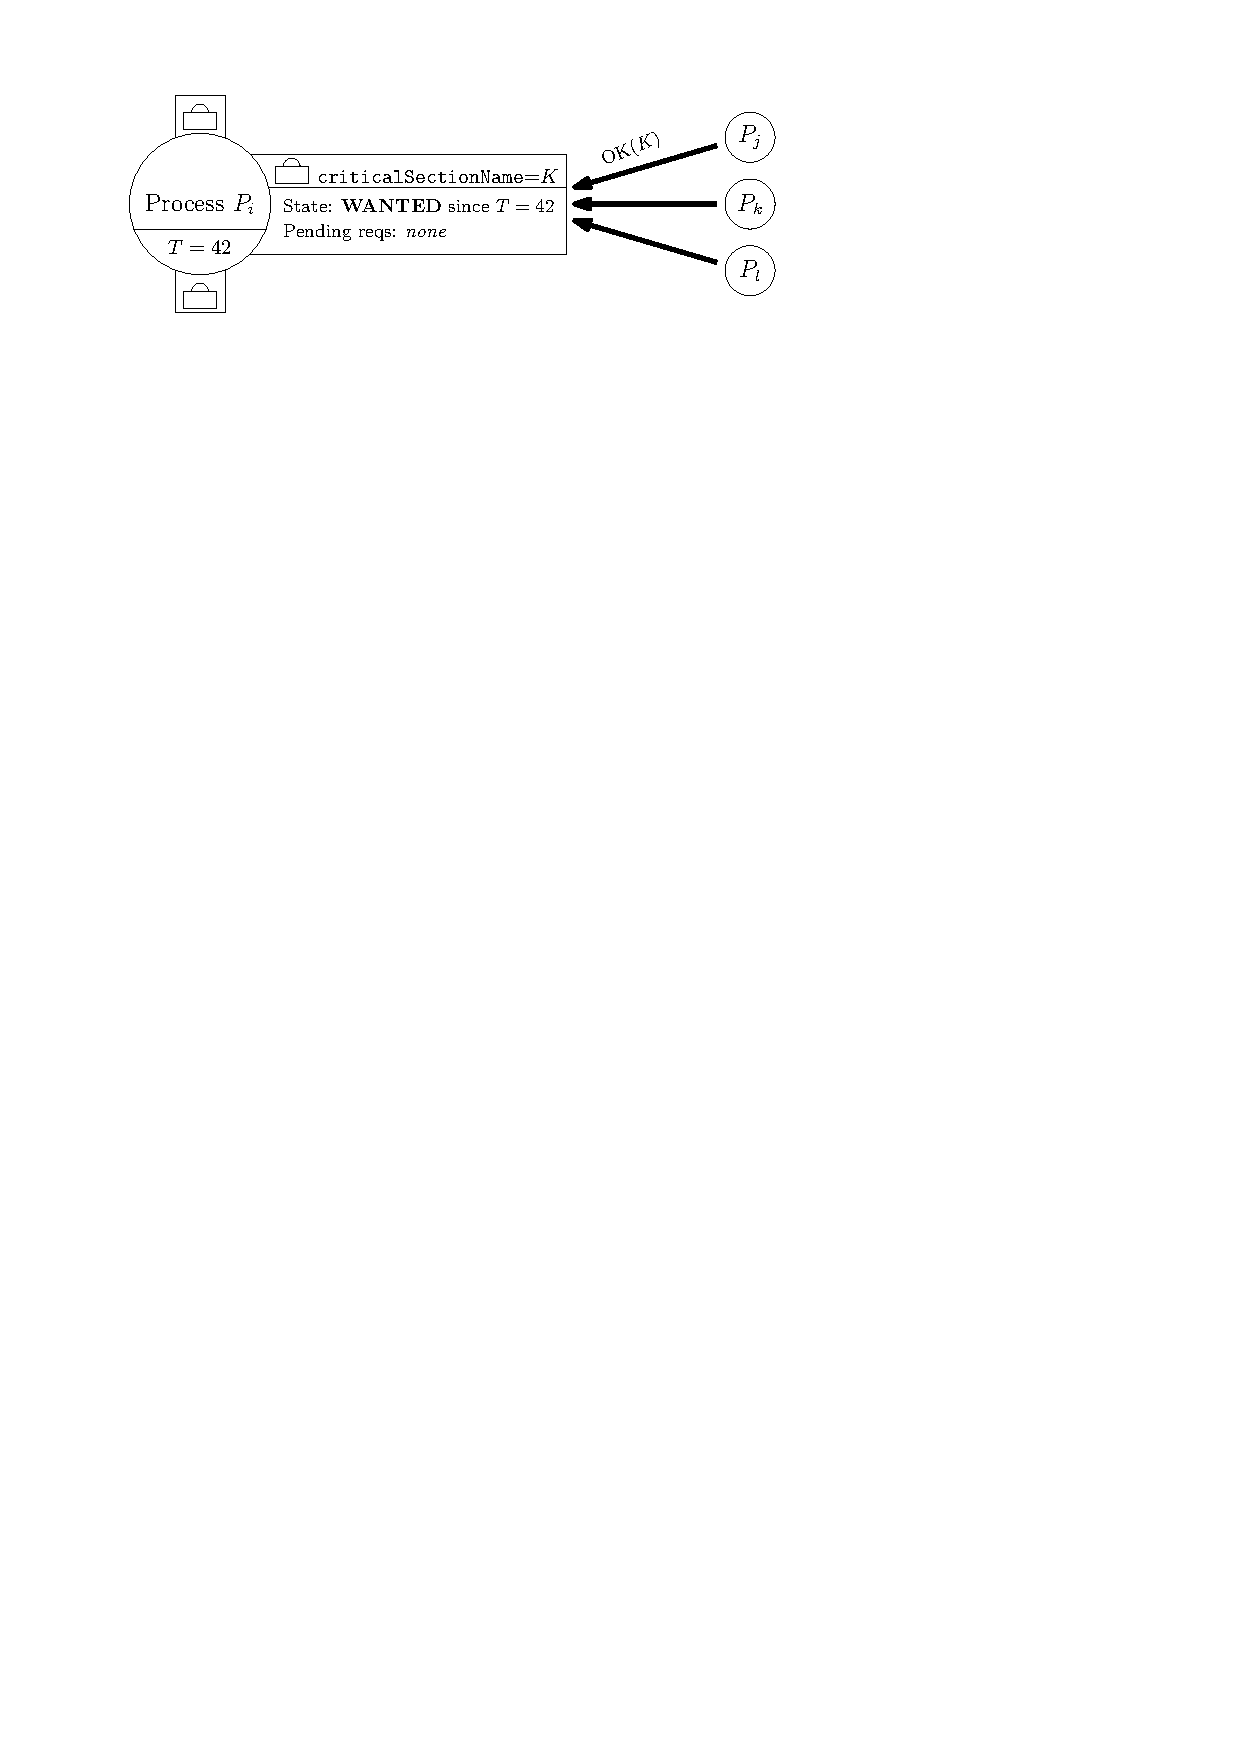
\includegraphics[width=0.95\linewidth]{11/figs/mutex_ok_3.pdf}}%
		\only<4>{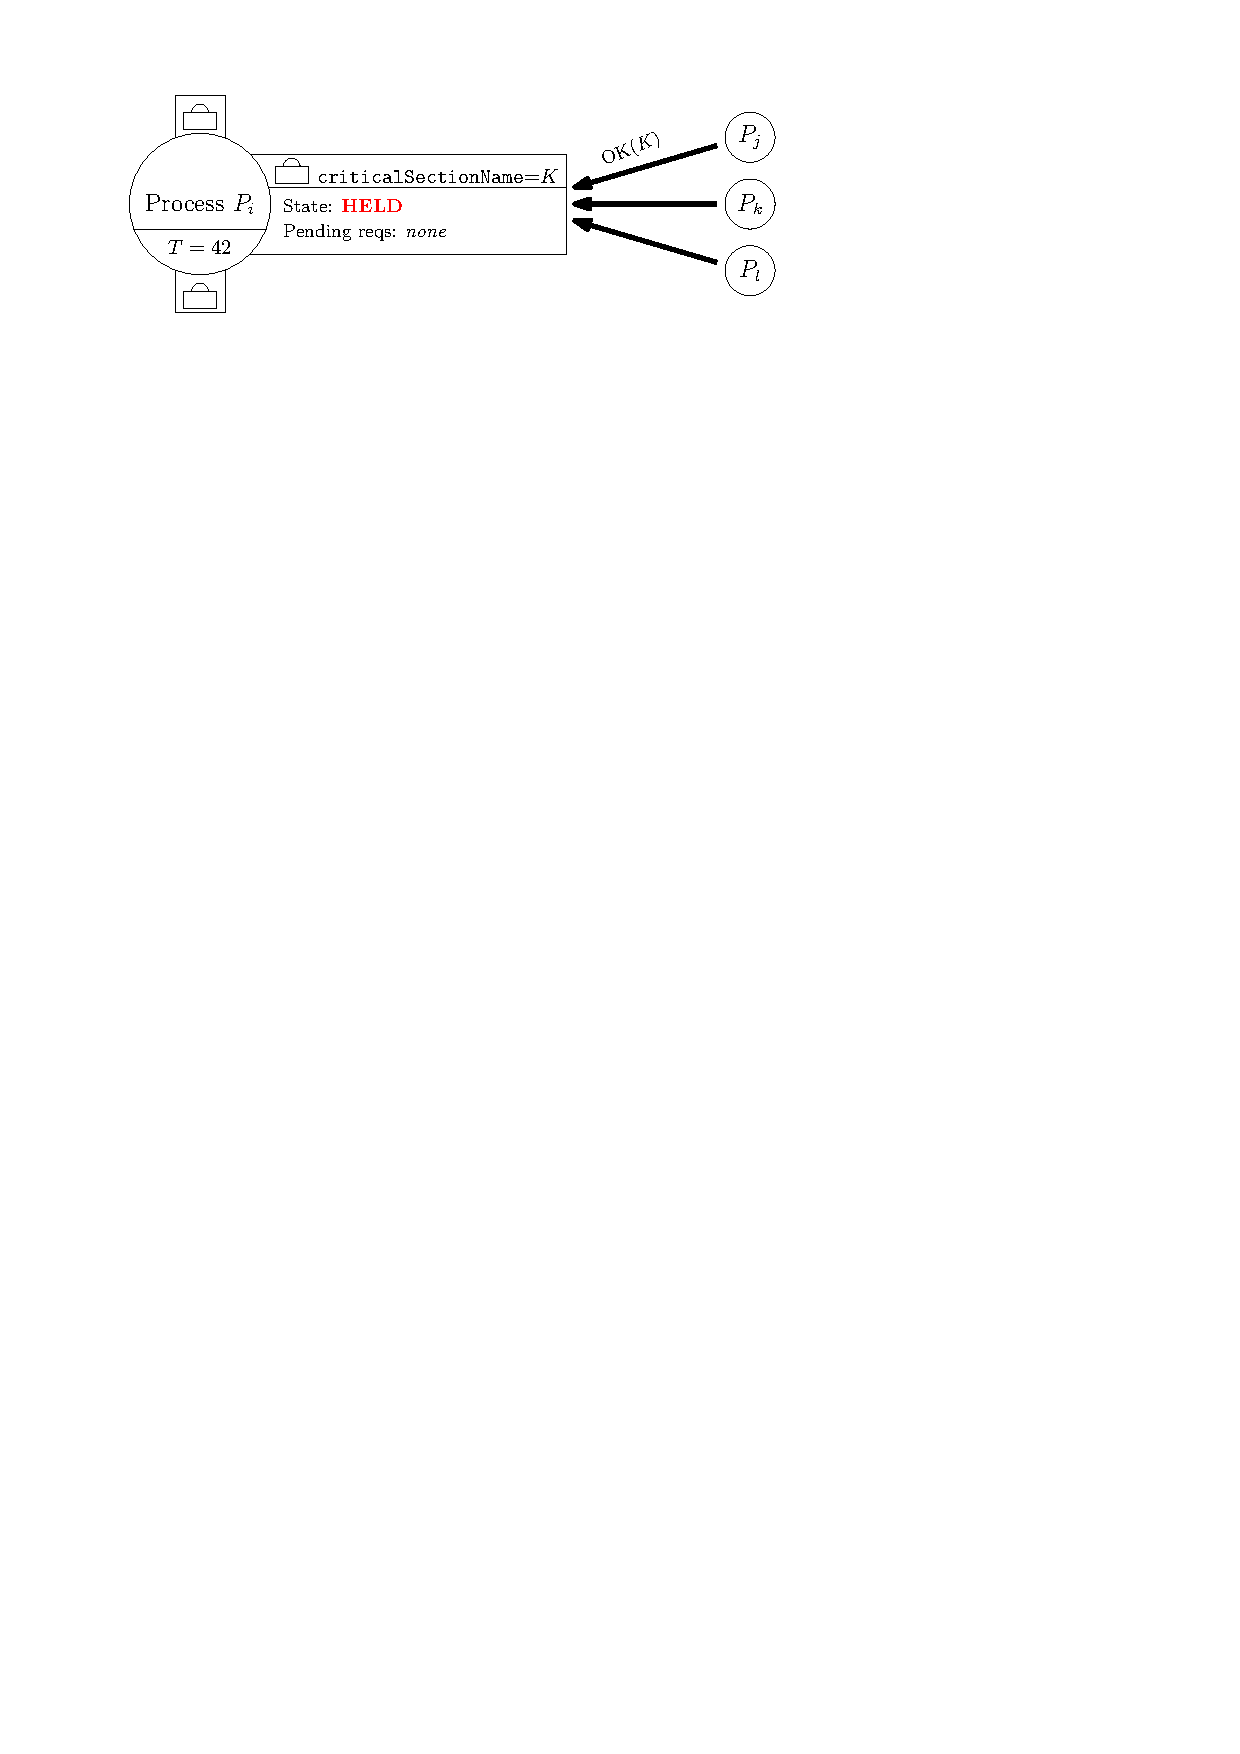
\includegraphics[width=0.95\linewidth]{11/figs/mutex_ok_4.pdf}}%
	\end{center}

	\only<4>{
		\vspace{2em}\hrule\vspace{1em}
		\begin{enumerate}
			\setcounter{enumi}{1}
			\item Zámek K procesu je ve stavu  {\bf WANTED} dokud neobdrží zprávu OK(K) od každého dalšího přistupujícího procesu. Poté se nastaví na  {\bf HELD}.
		\end{enumerate}
	}
\end{frame}


\begin{frame}[t]
	\frametitle{Příchozí požadavek od jiného procesu}
	\vspace{1.8em}
	\begin{center}
		\only<1>{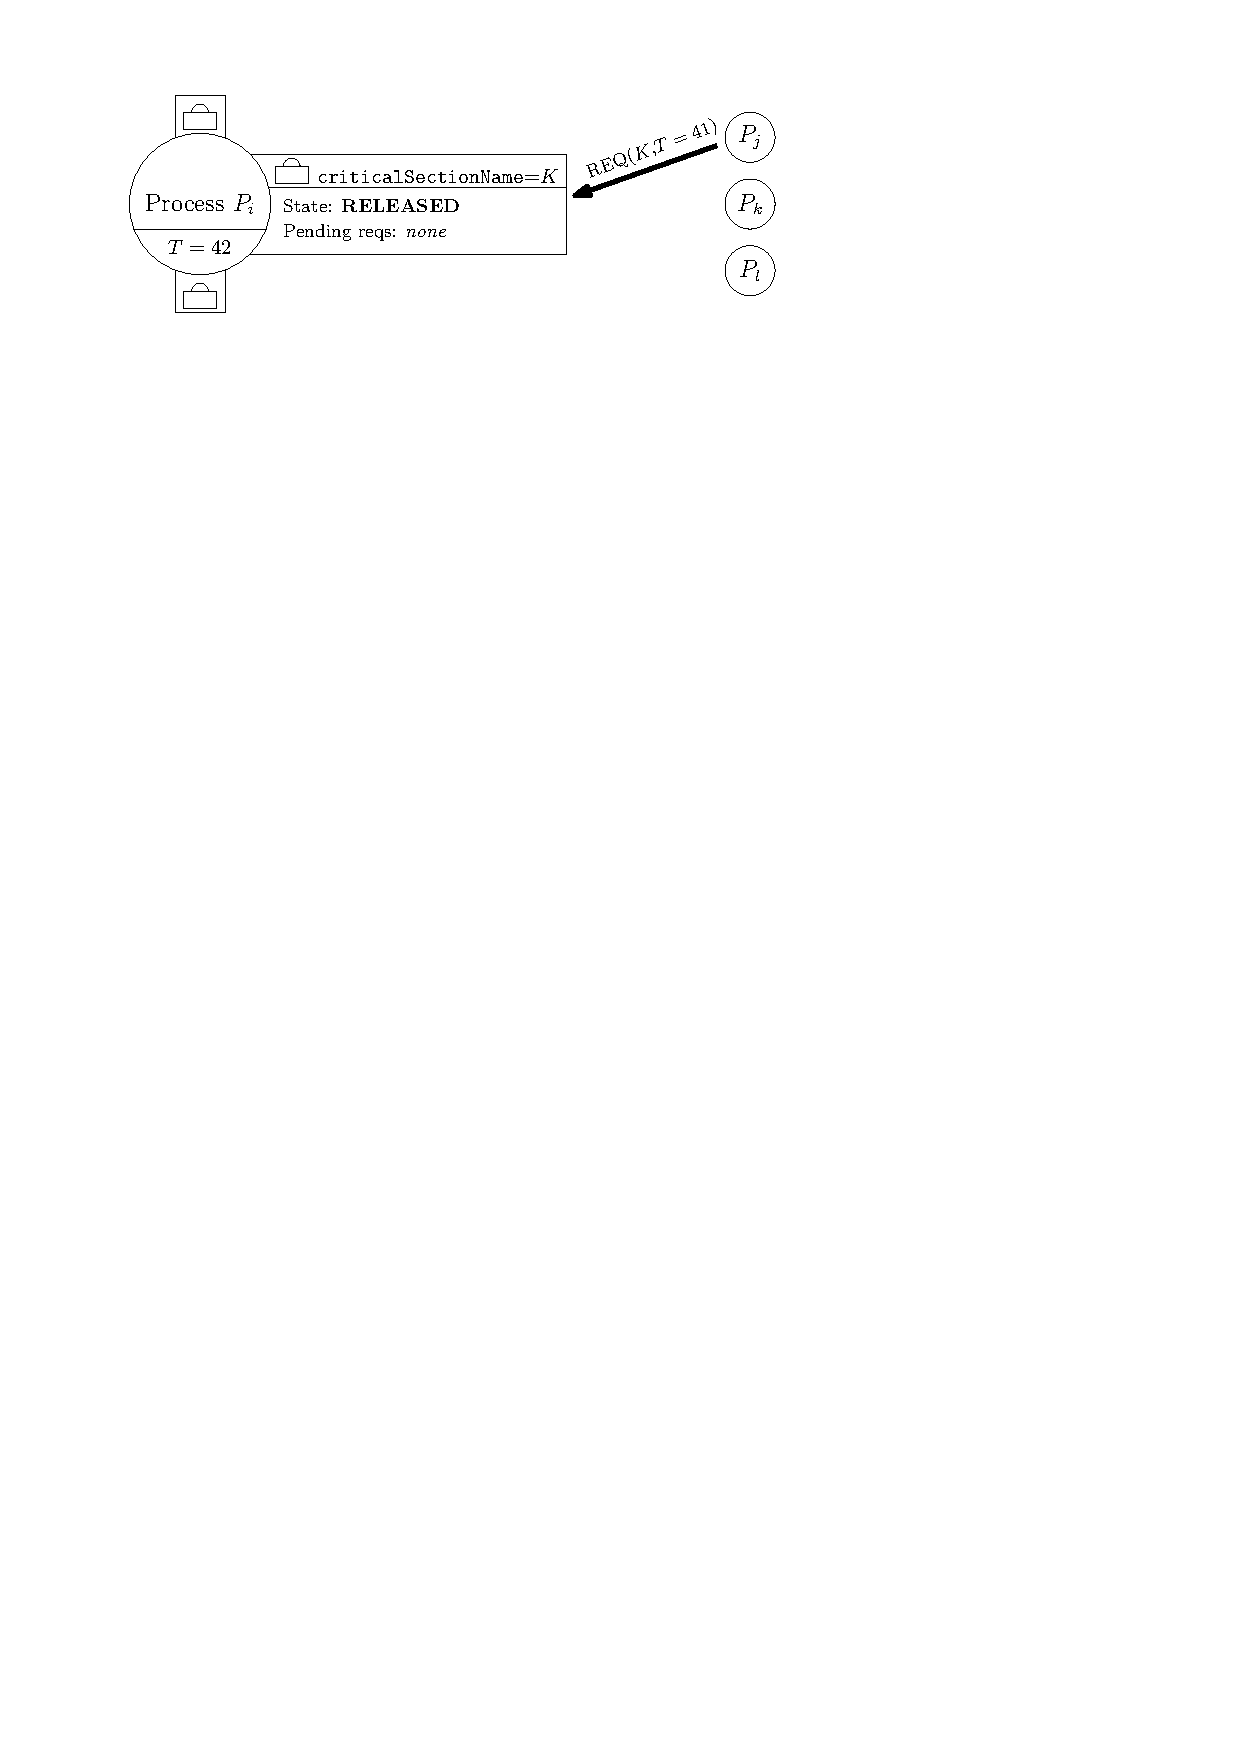
\includegraphics[width=0.95\linewidth]{11/figs/mutex_oreq_released_1.pdf}}%
		\only<2>{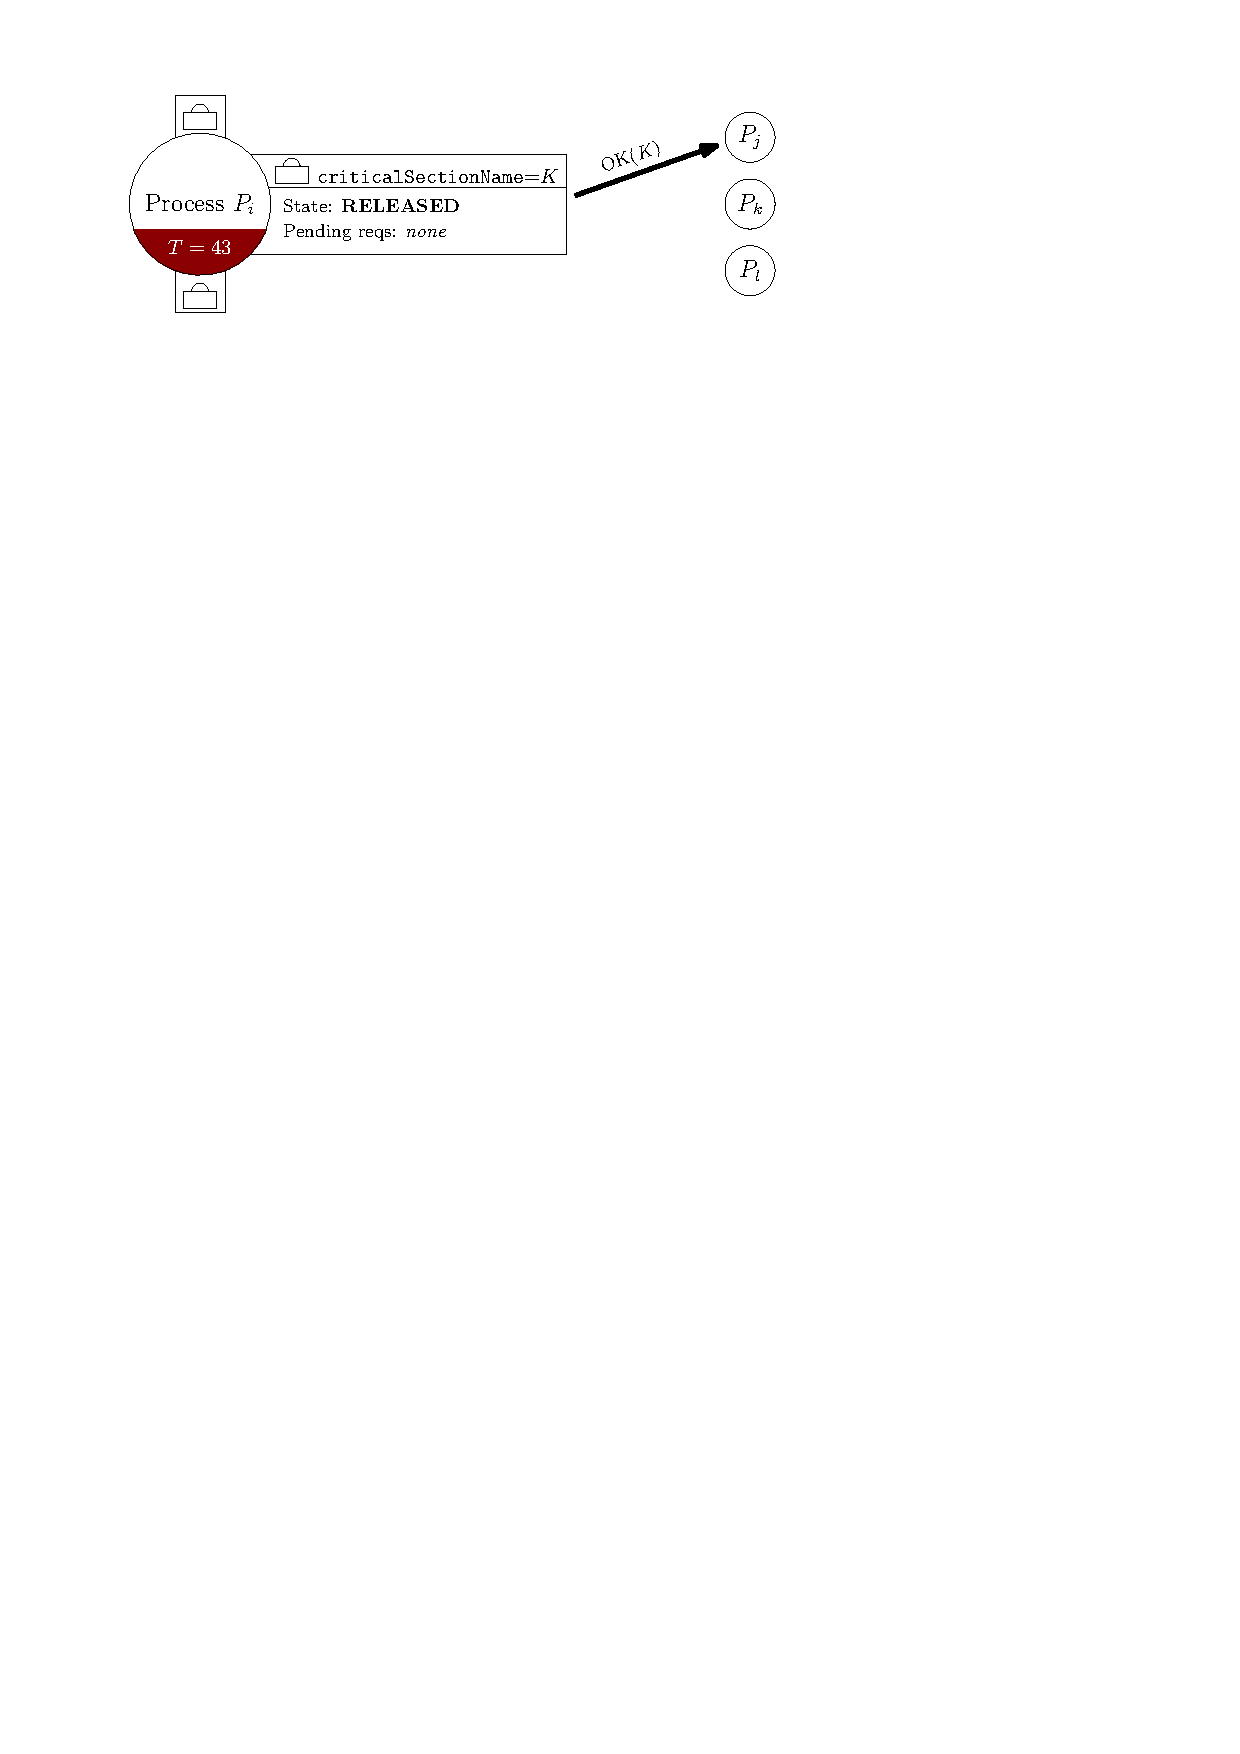
\includegraphics[width=0.95\linewidth]{11/figs/mutex_oreq_released_2.pdf}}%
		\only<3>{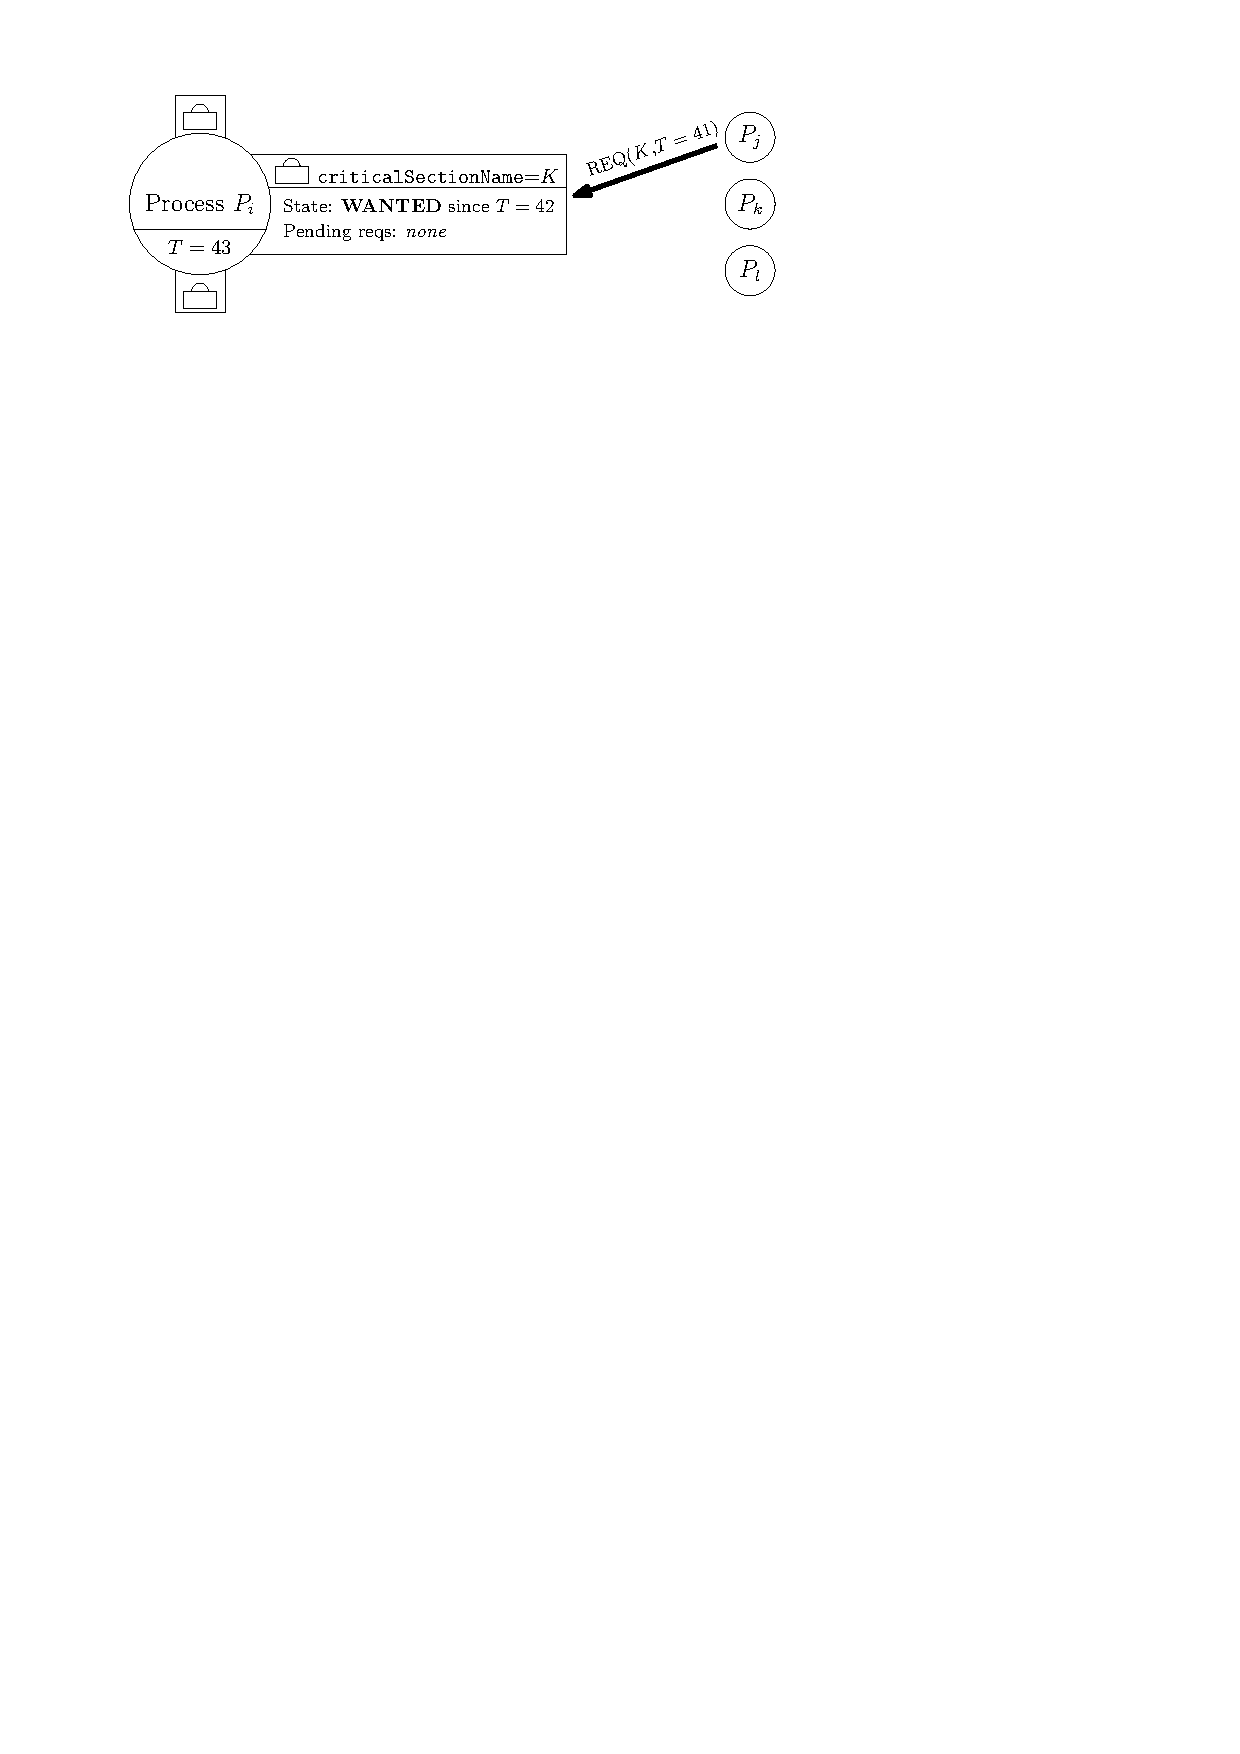
\includegraphics[width=0.95\linewidth]{11/figs/mutex_oreq_higherprio_1.pdf}}%
		\only<4>{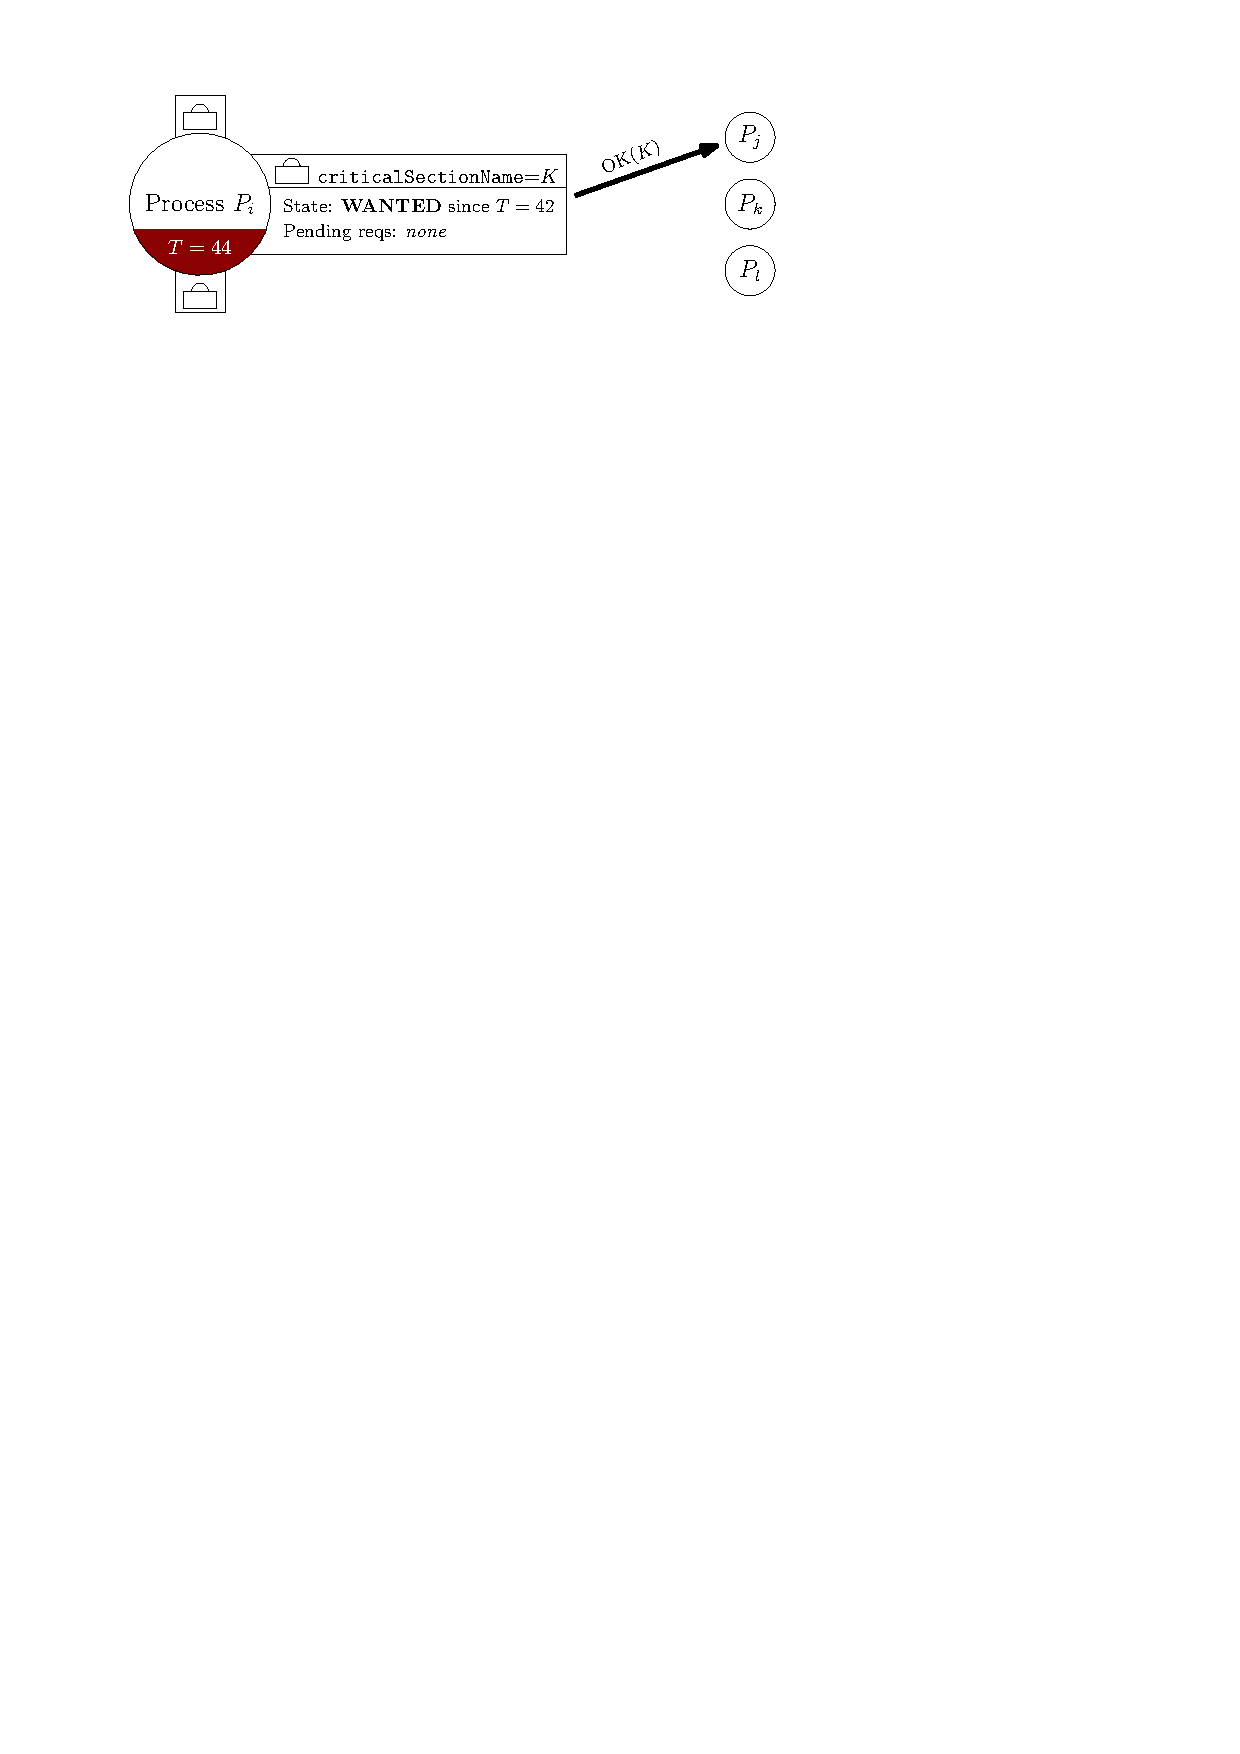
\includegraphics[width=0.95\linewidth]{11/figs/mutex_oreq_higherprio_2.pdf}}%
	\end{center}

	\only<4>{
		\vspace{2em}\hrule\vspace{1em}
		\begin{enumerate}
			\setcounter{enumi}{2}
			\item Pokud procesu $P_i$ přijde zpráva REQUEST(K) od procesu $P_j$ s časem $T_j$:
						\begin{enumerate}
							\item[(i)] pokud je zámek K ve stavu  {\bf RELEASED}, nebo je ve stavu {\bf WANTED} a o vstup do kritické sekce žádal v čase $T_i > T_j$, pak pošle zprávu OK(K) procesu $P_j$,
						\end{enumerate}
		\end{enumerate}
	}
\end{frame}

\begin{frame}[t]
	\frametitle{Příchozí požadavek od jiného procesu}
	\vspace{1.8em}
	\begin{center}
		\only<1>{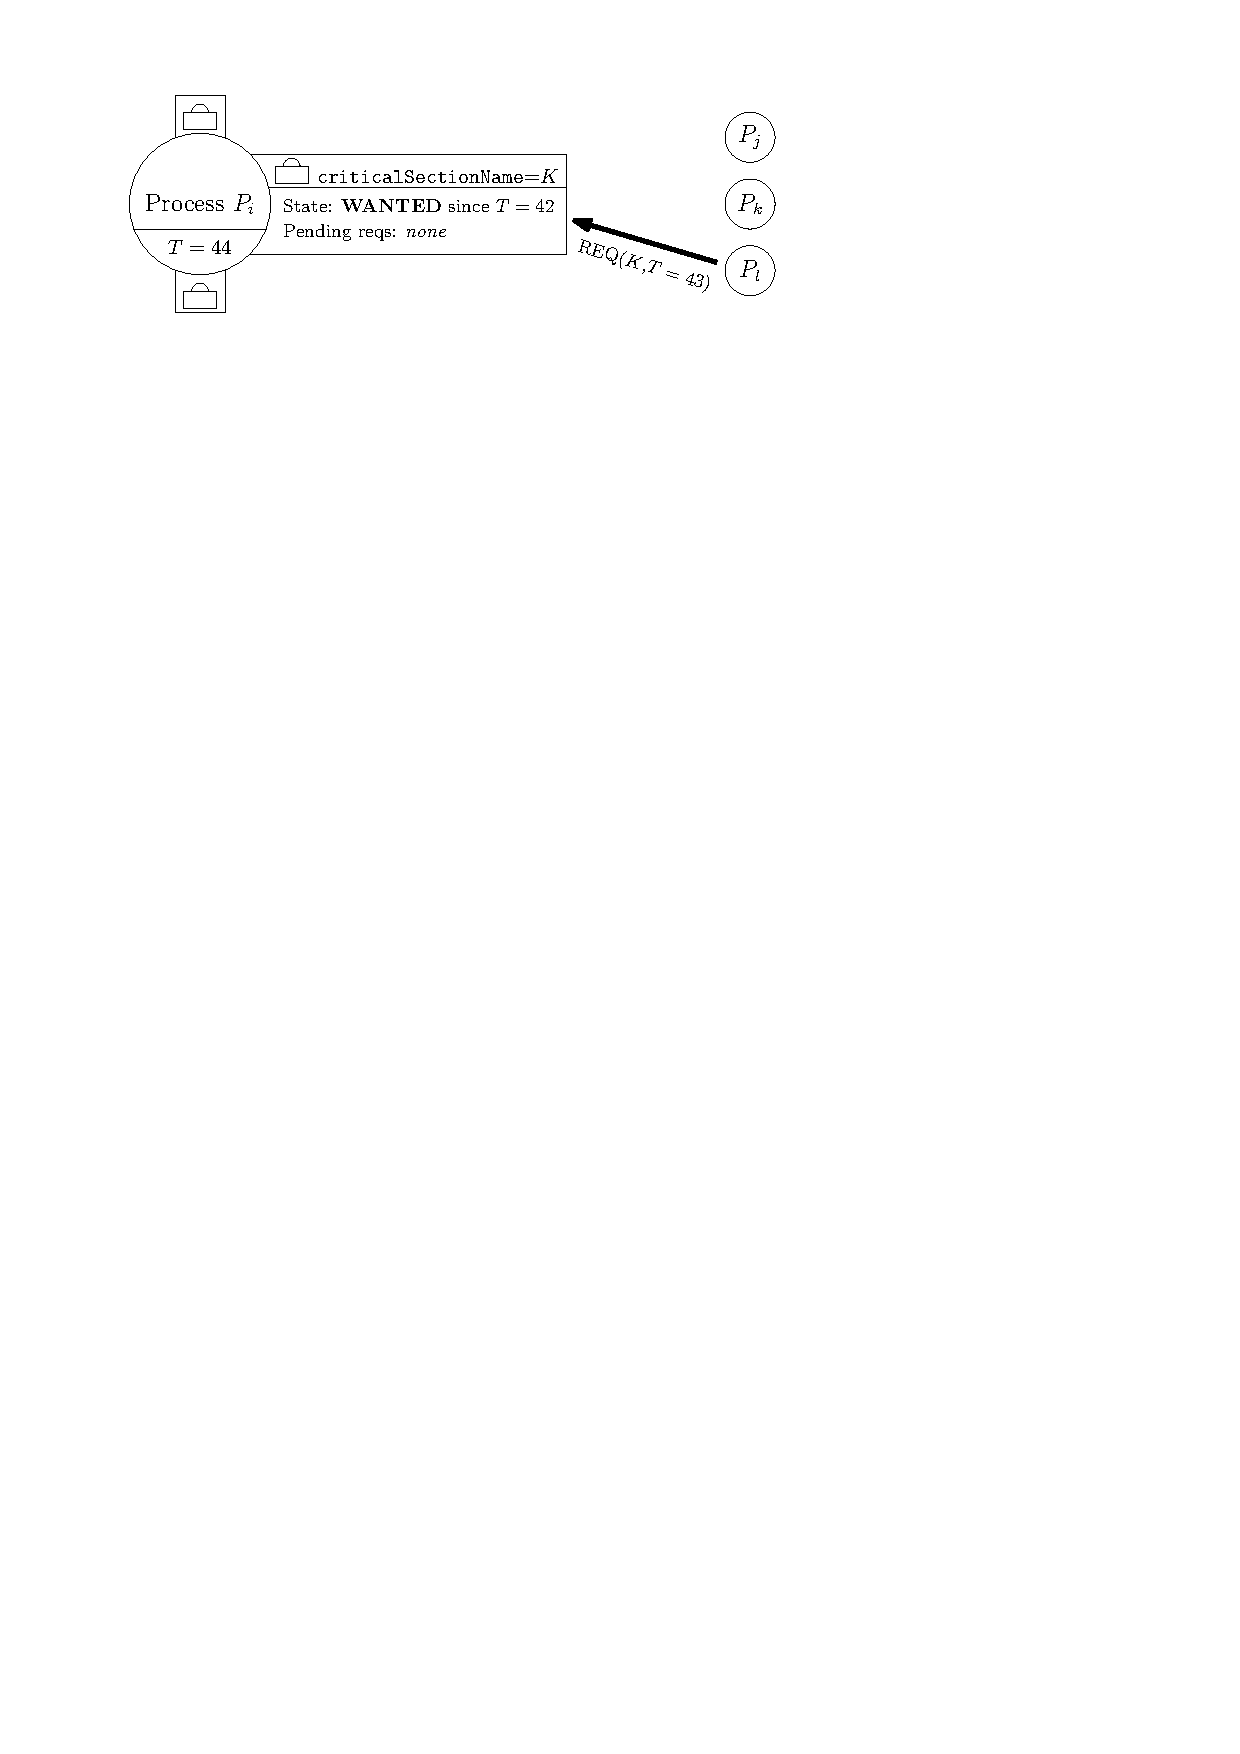
\includegraphics[width=0.95\linewidth]{11/figs/mutex_oreq_lowerprio_1.pdf}}%
		\only<2>{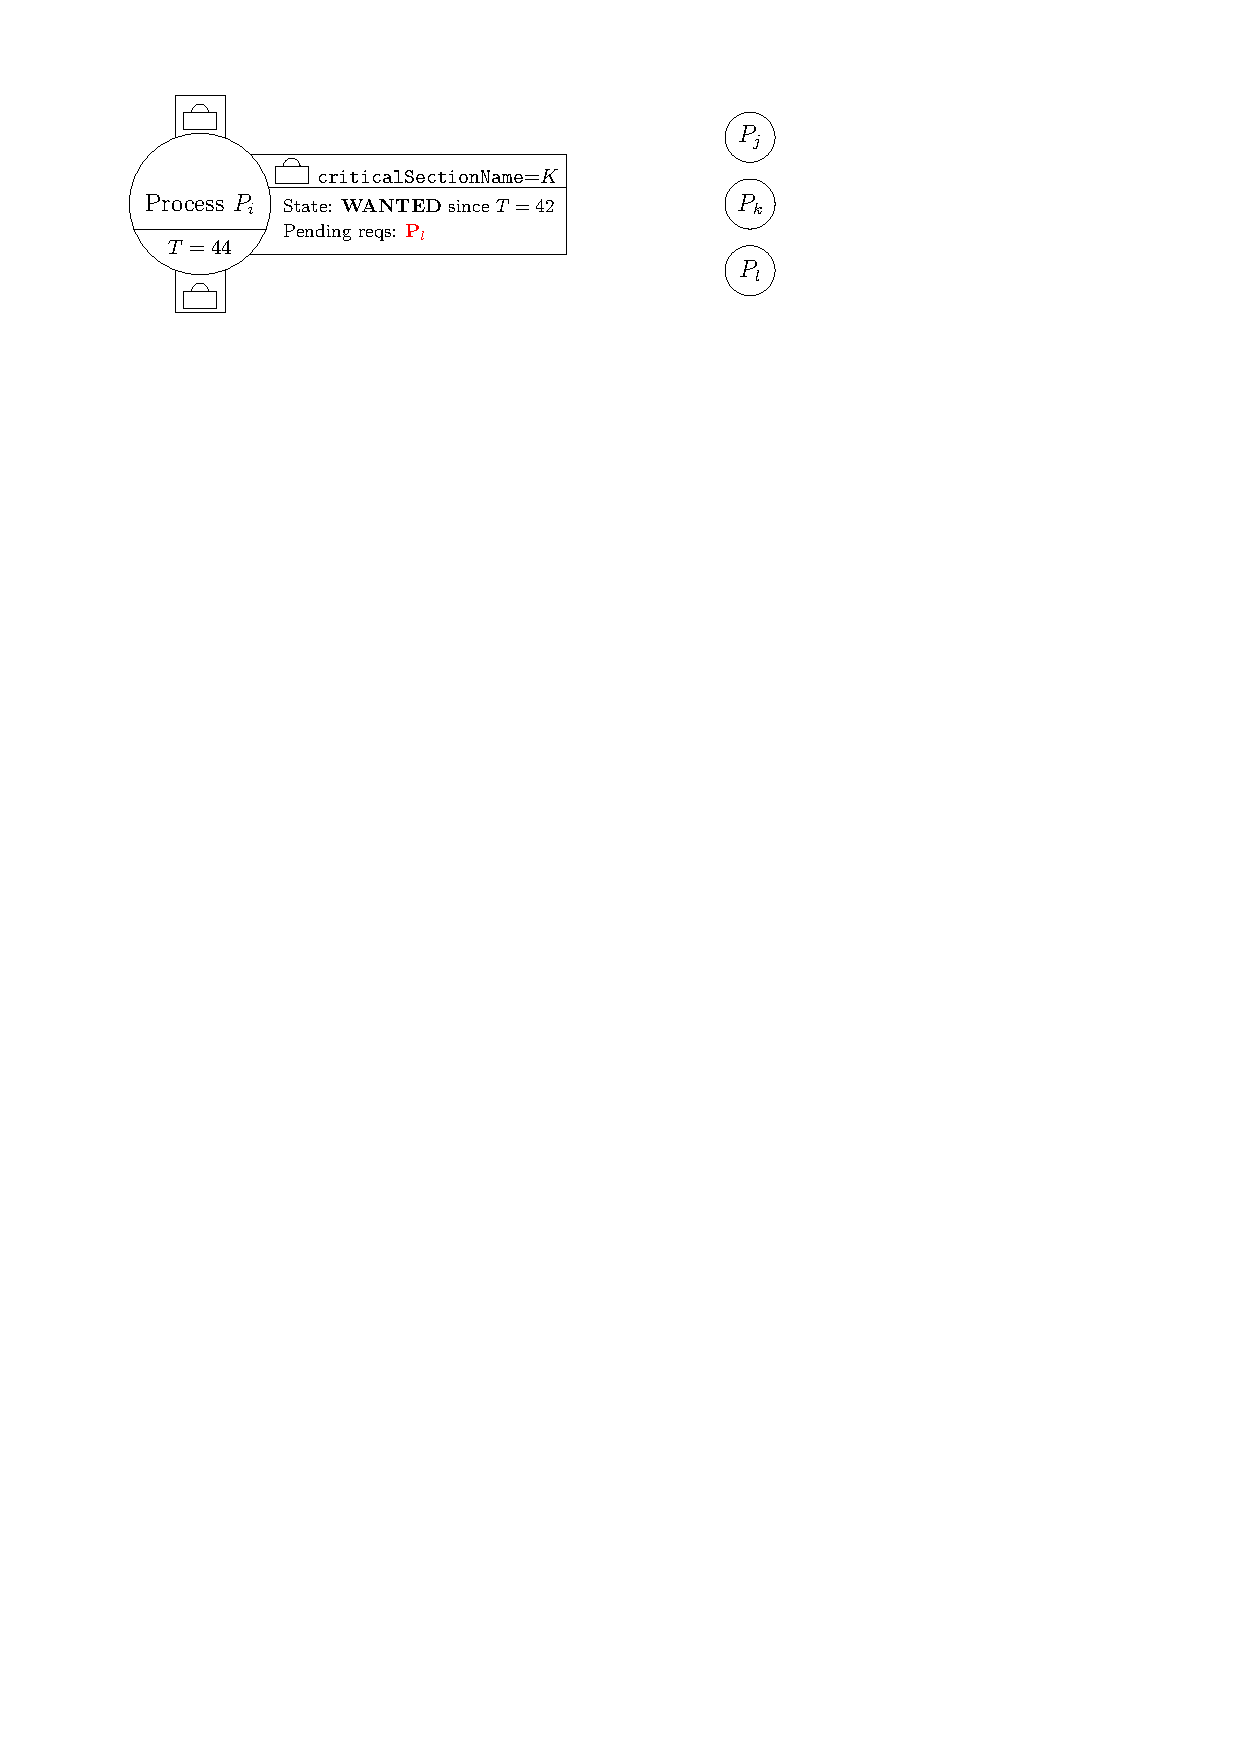
\includegraphics[width=0.95\linewidth]{11/figs/mutex_oreq_lowerprio_2.pdf}}%
		\only<3>{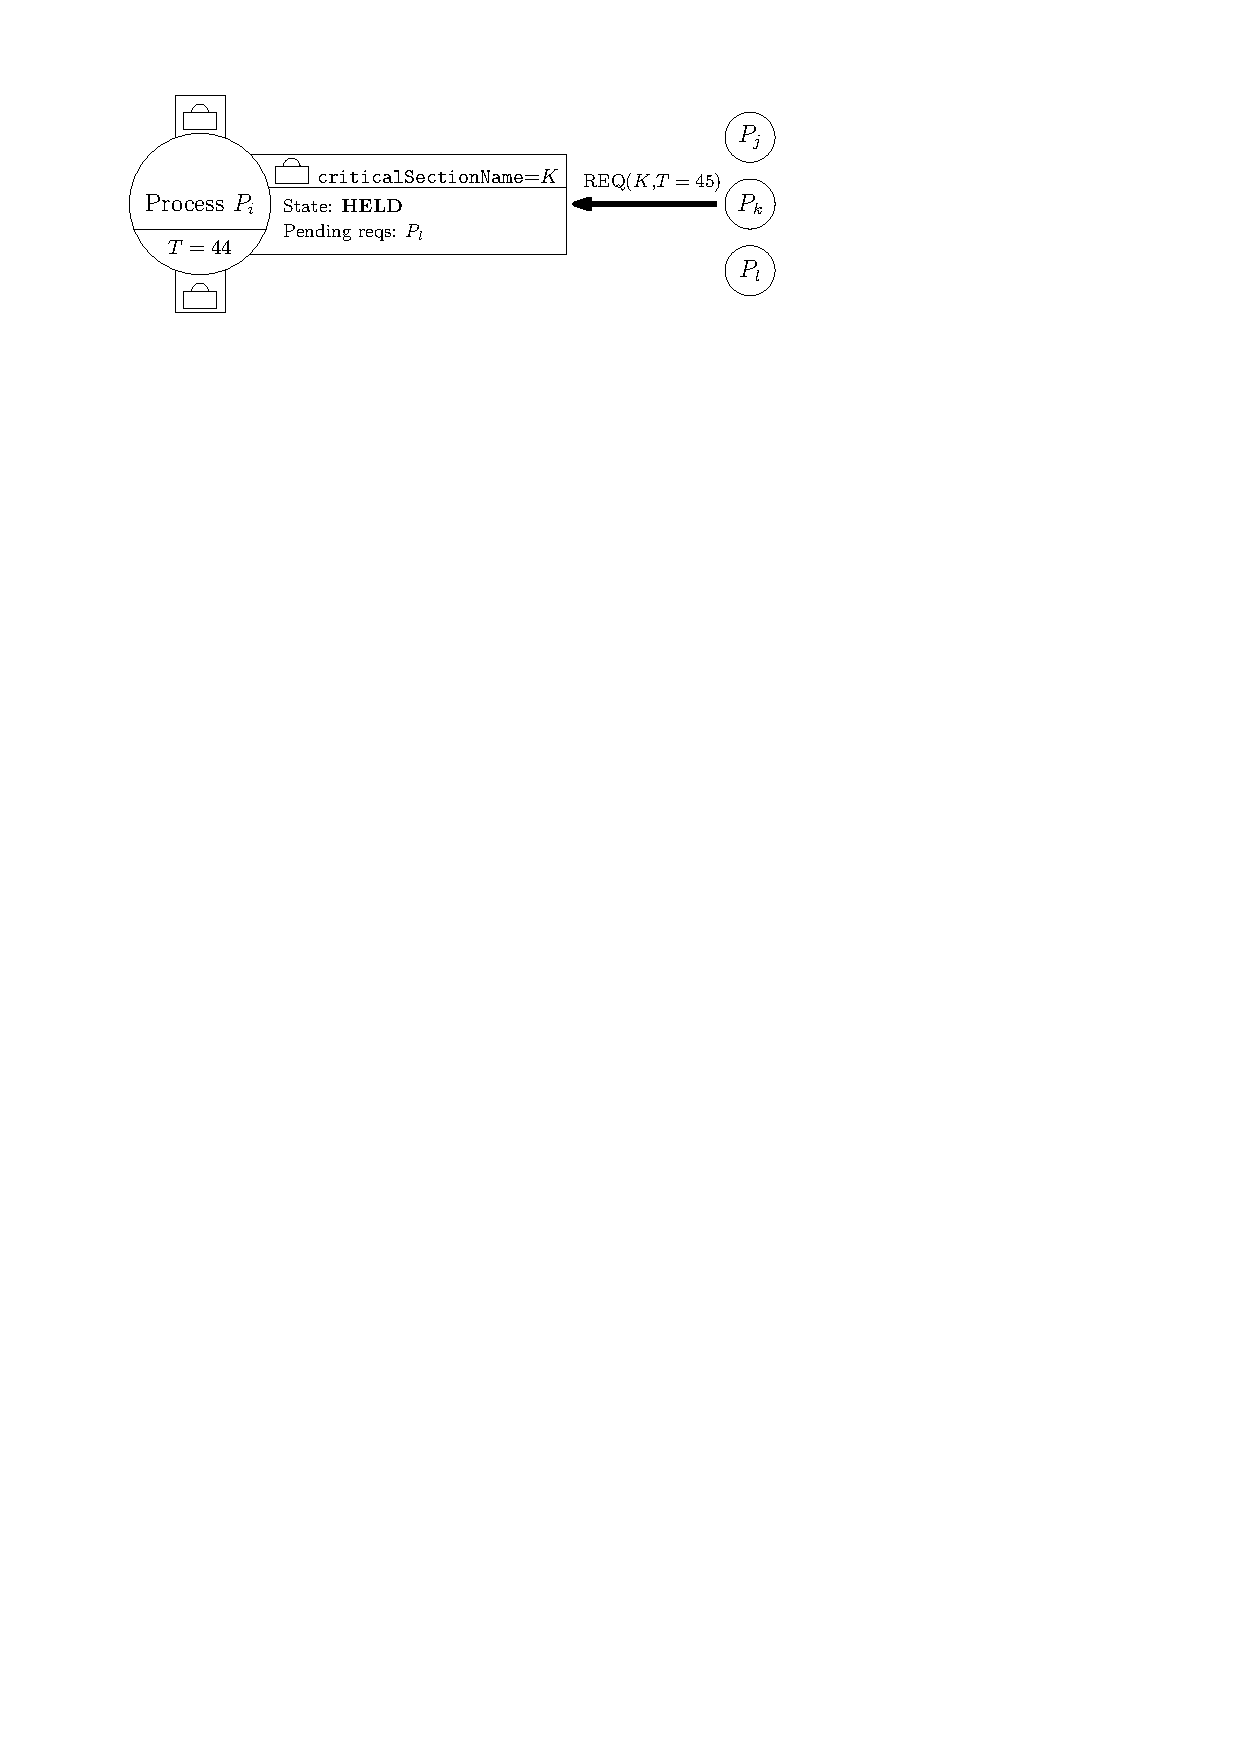
\includegraphics[width=0.95\linewidth]{11/figs/mutex_oreq_held_1.pdf}}%
		\only<4>{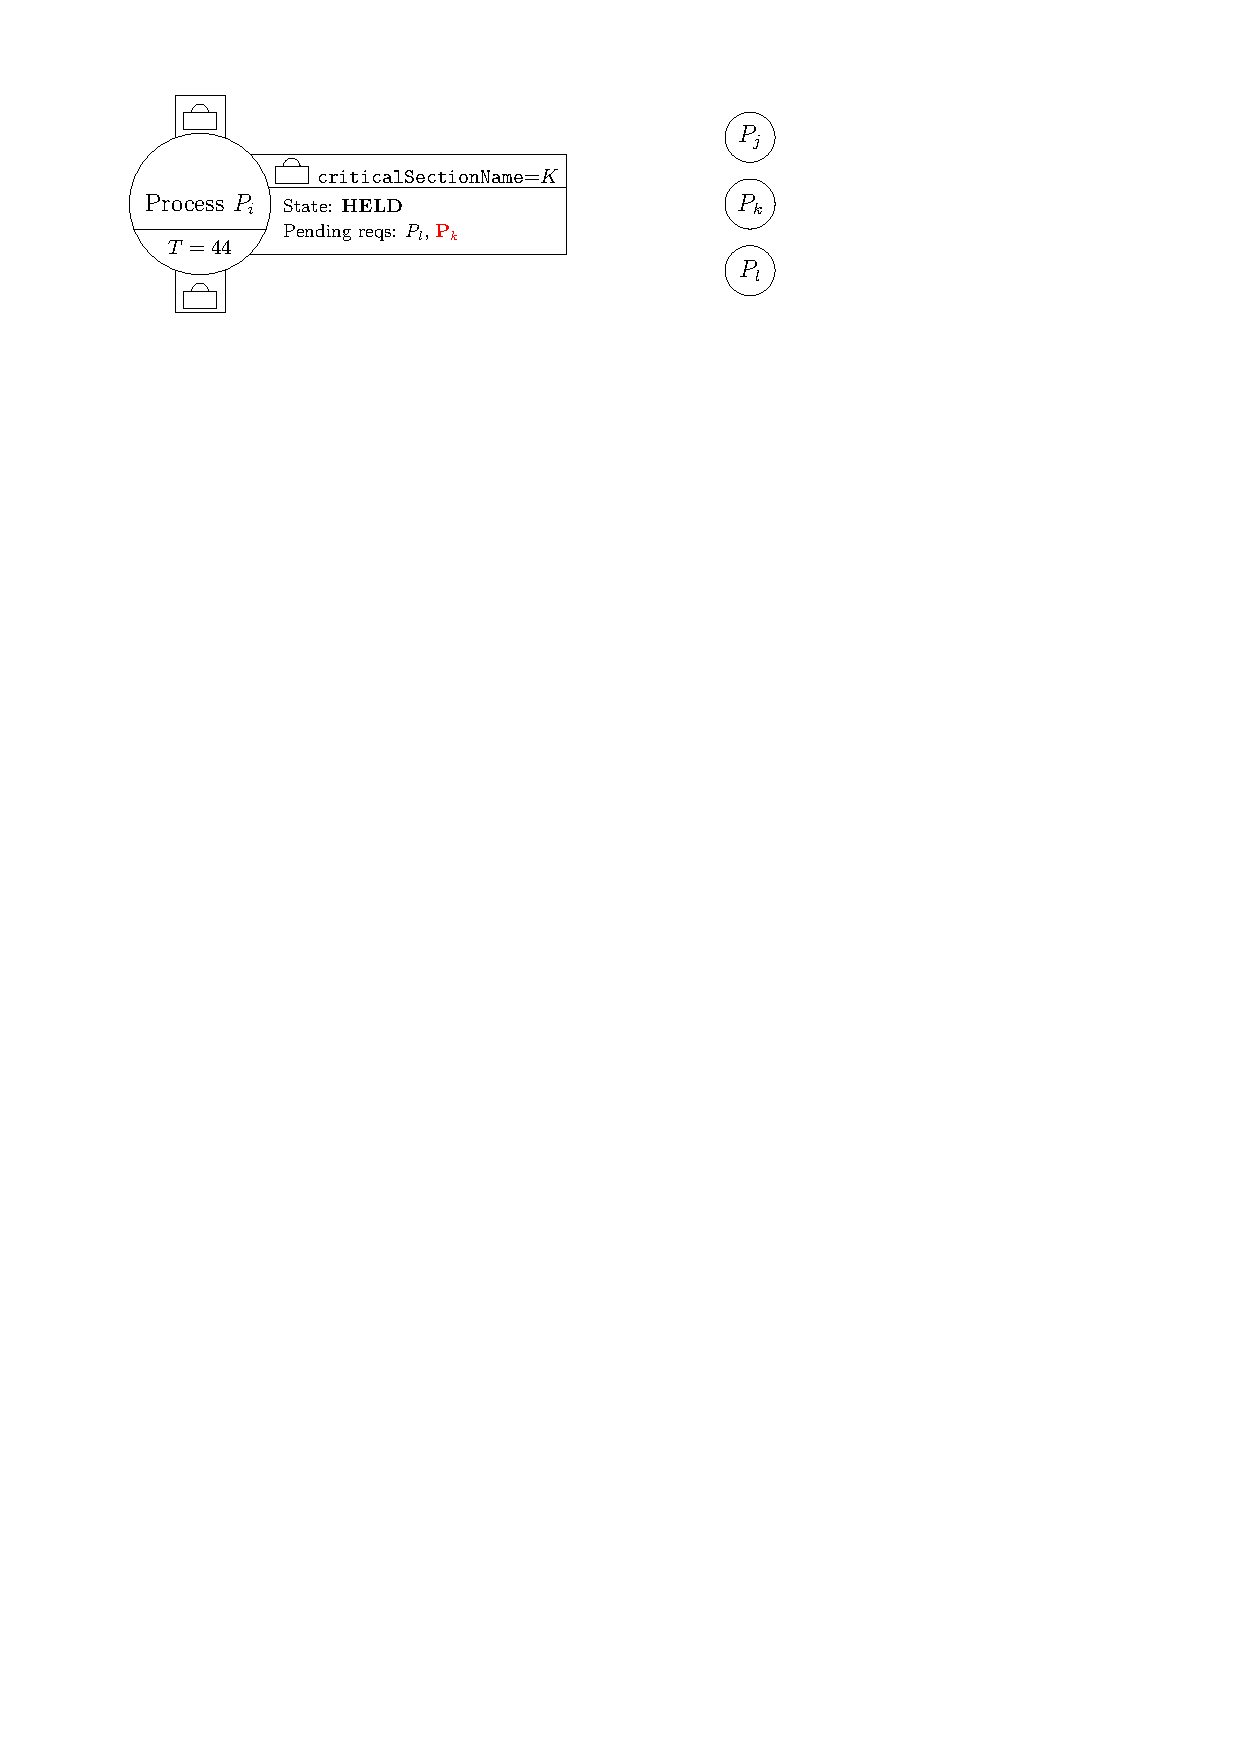
\includegraphics[width=0.95\linewidth]{11/figs/mutex_oreq_held_2.pdf}}%
	\end{center}

	\only<4>{
		\vspace{2em}\hrule\vspace{1em}
		\begin{enumerate}
			\setcounter{enumi}{2}
			\item Pokud procesu $P_i$ přijde zpráva REQUEST(K) od procesu $P_j$ s časem $T_j$:
						\begin{enumerate}
							\item[(ii)] jinak požadavek odloží a neodpoví.
						\end{enumerate}
		\end{enumerate}
	}
\end{frame}


\begin{frame}[t]
	\frametitle{Opuštění kritické sekce}
	\vspace{1.8em}
	\begin{center}
		\only<1>{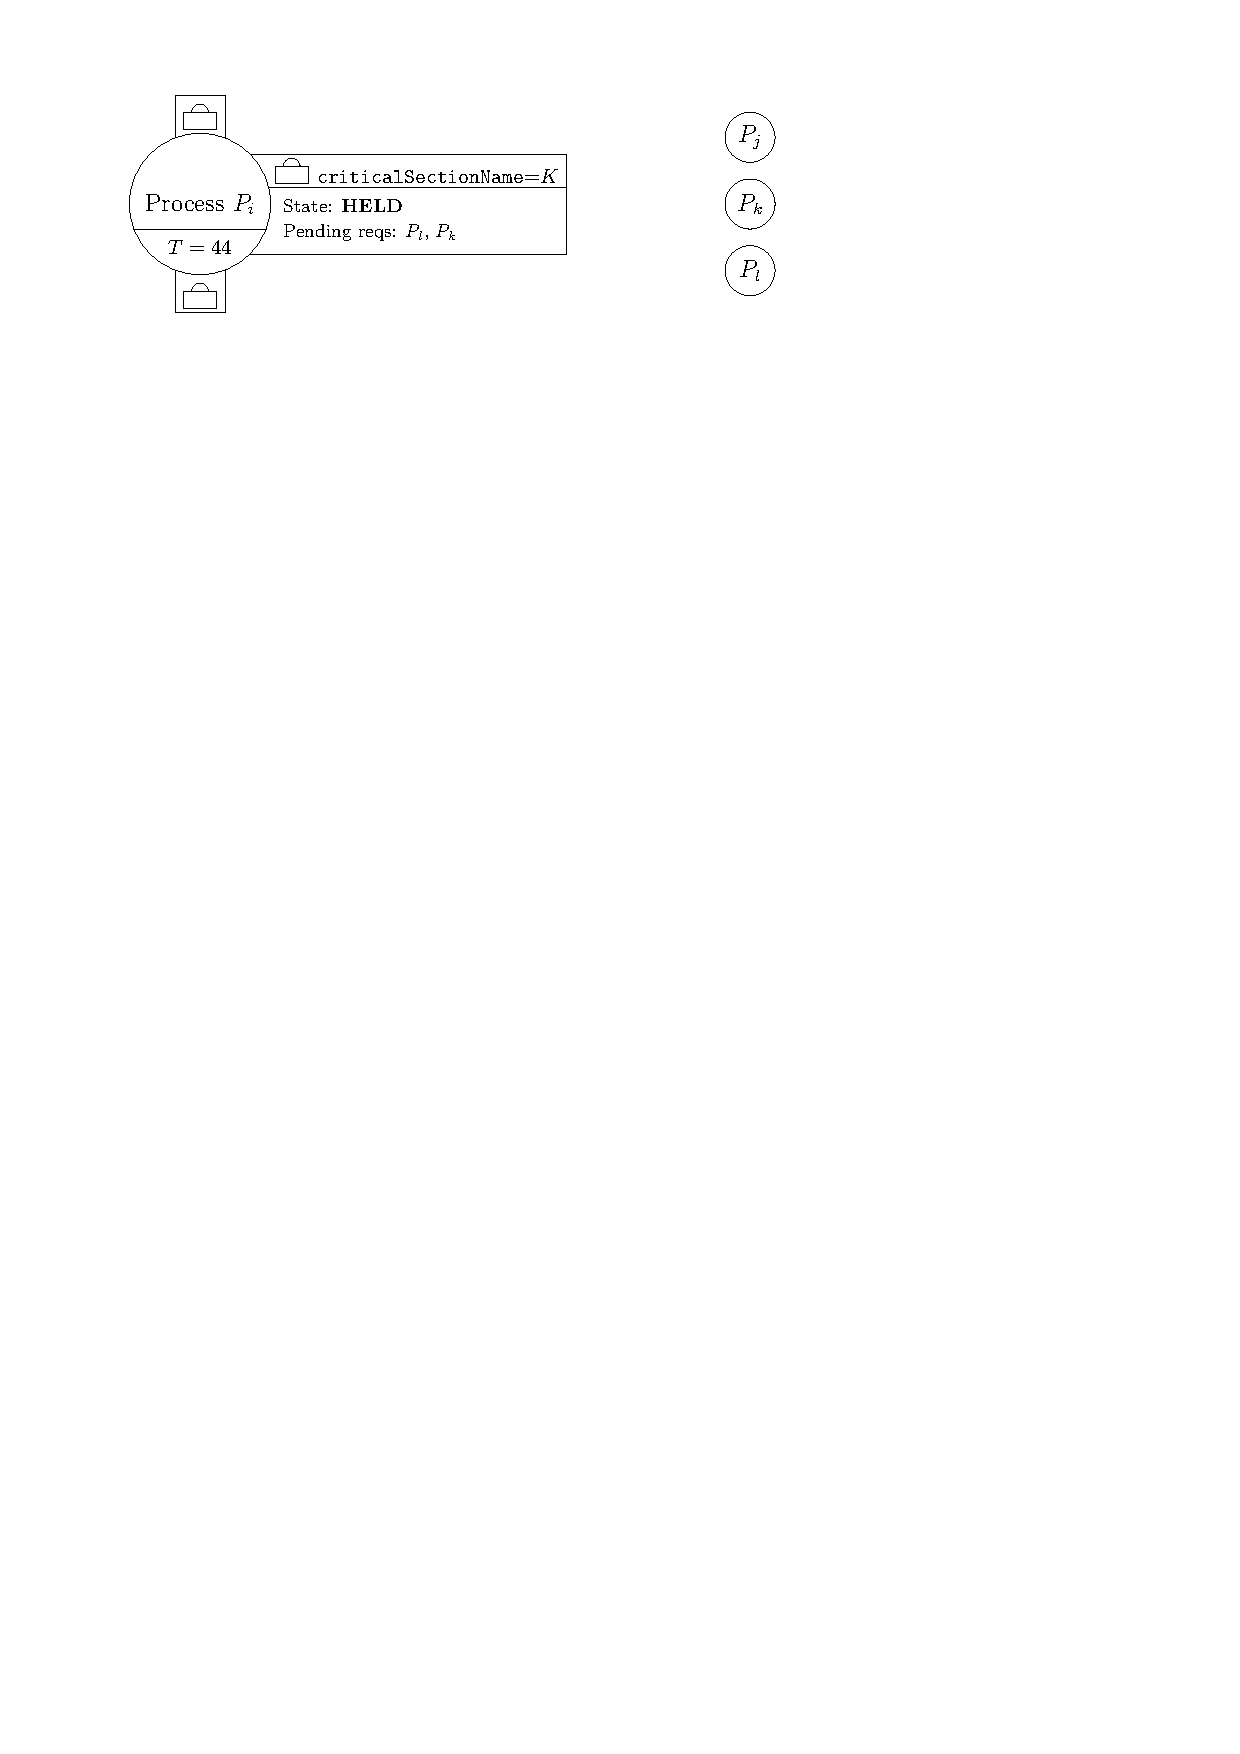
\includegraphics[width=0.95\linewidth]{11/figs/mutex_oreq_release_1.pdf}}%
		\only<2>{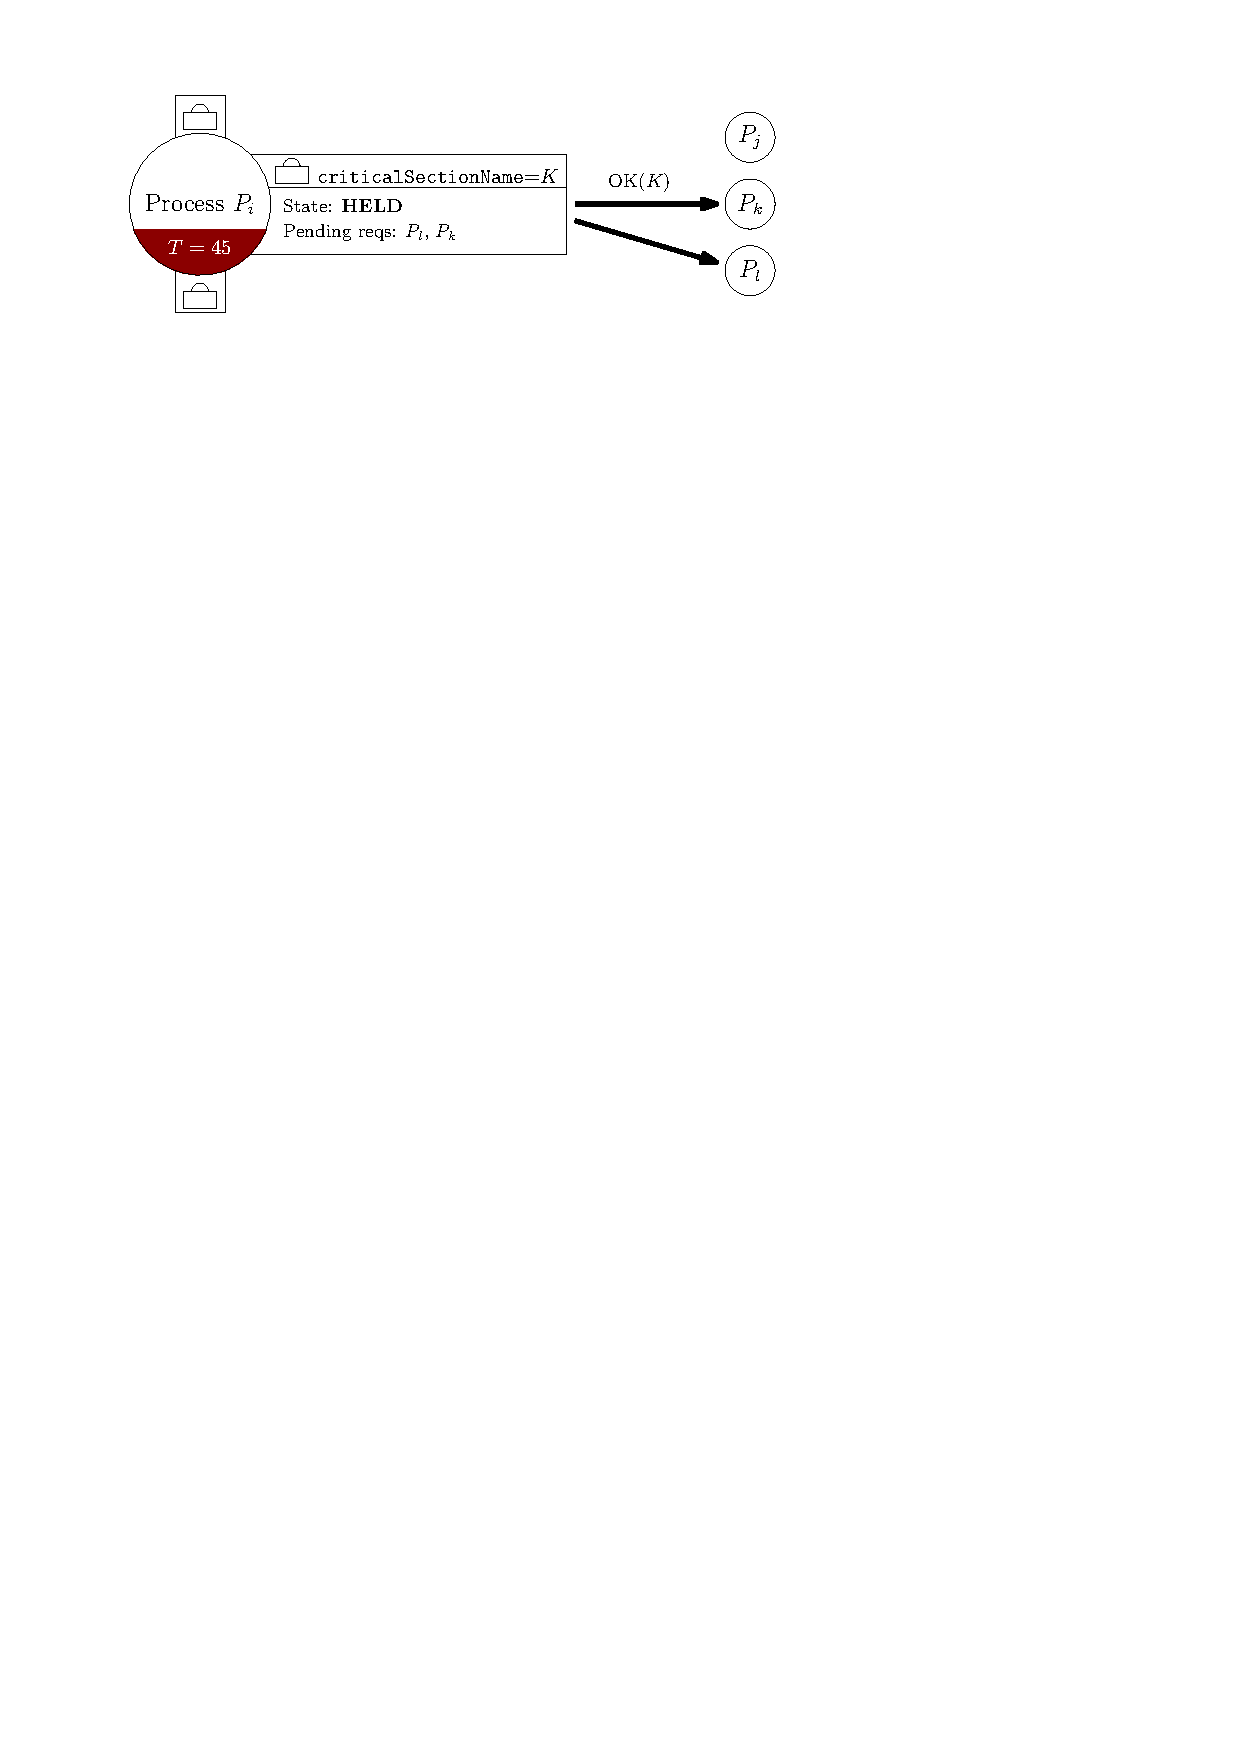
\includegraphics[width=0.95\linewidth]{11/figs/mutex_oreq_release_2.pdf}}%
		\only<3>{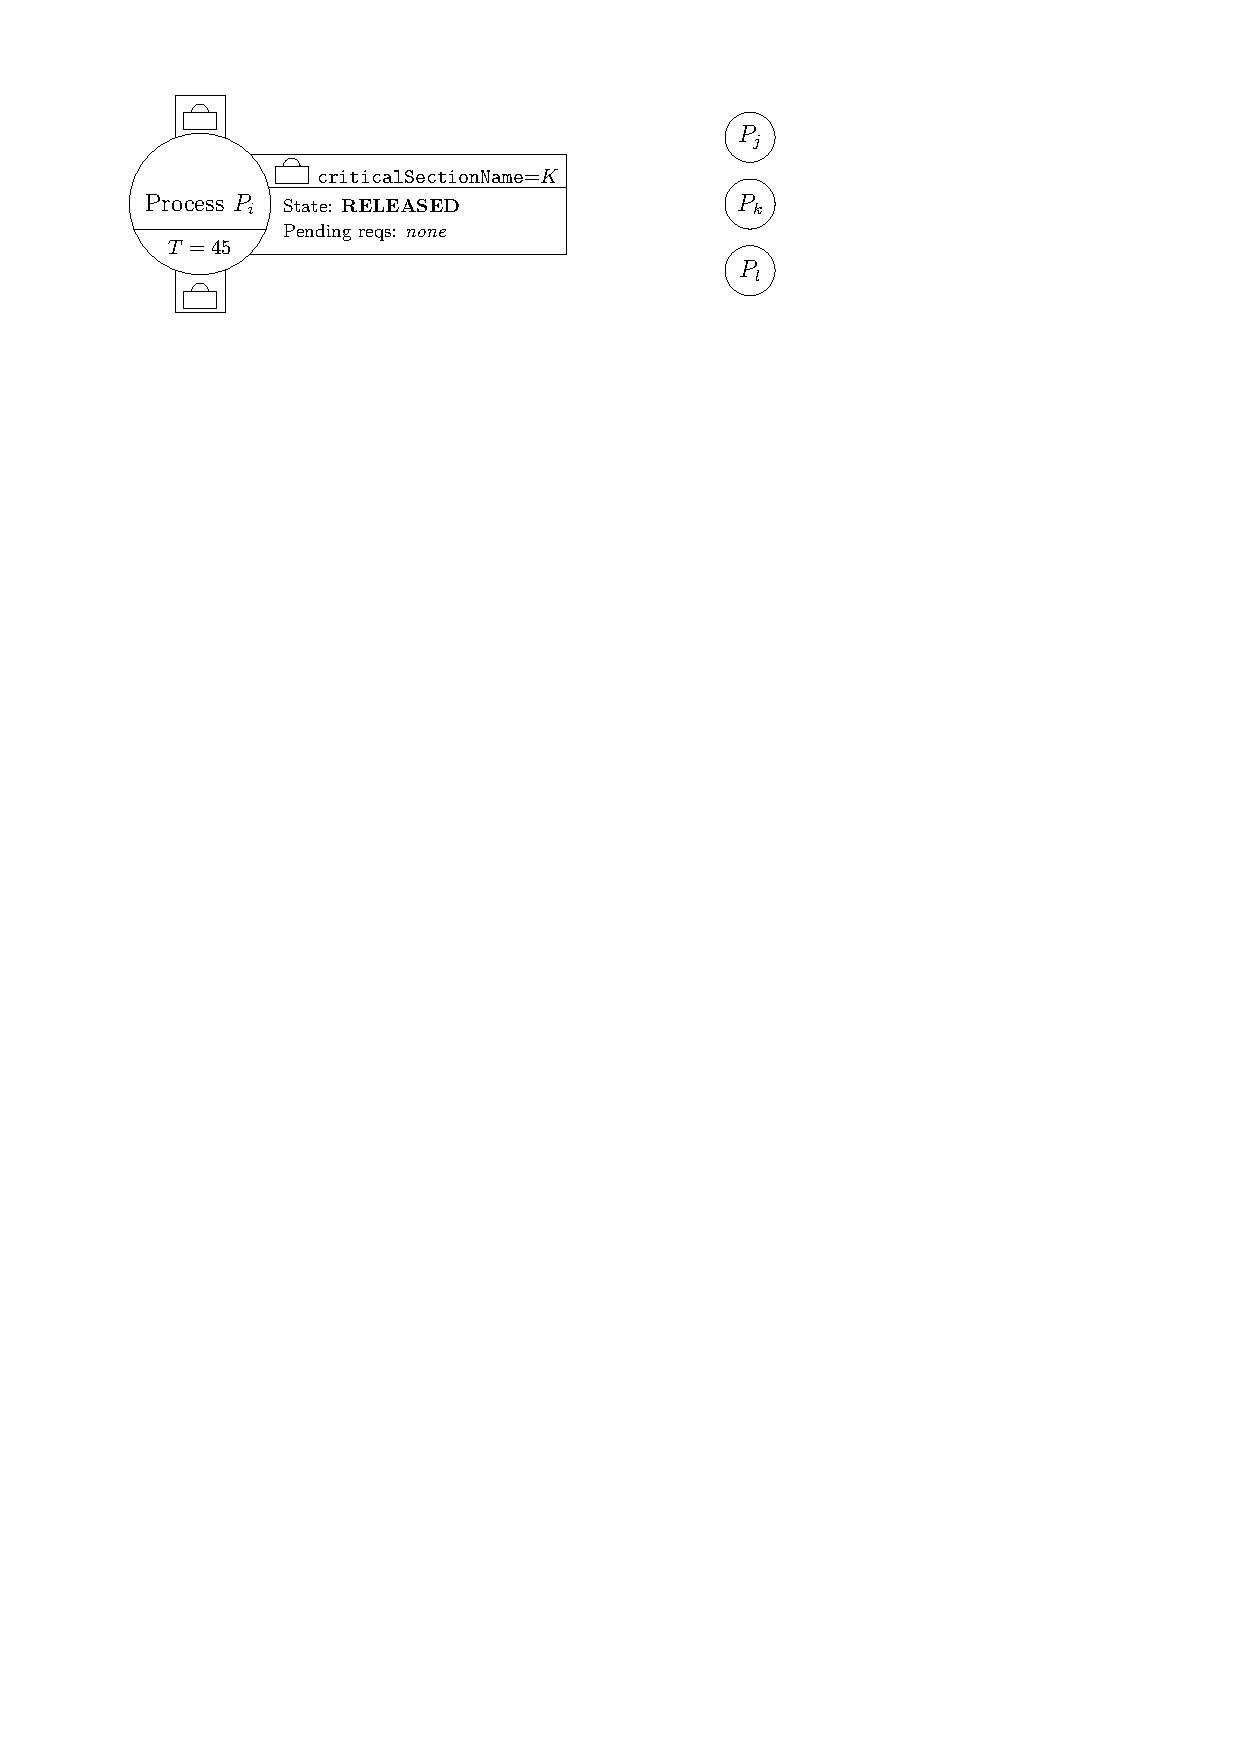
\includegraphics[width=0.95\linewidth]{11/figs/mutex_oreq_release_3.pdf}}%
	\end{center}

	\only<3>{
		\vspace{2em}\hrule\vspace{1em}
		\begin{enumerate}
			\setcounter{enumi}{3}
			\item Pokud proces $P_i$ dokončí práci v kritické sekci K, nastaví stav zámku K na {\bf RELEASED}, odpoví na všechny odložené požadavky a frontu požadavků vyprázdní.
		\end{enumerate}
	}
\end{frame}

\begin{frame}

\begin{center}
\Large Jaké požadavky tento algoritmus splňuje?
\end{center}

\begin{minipage}{0.4\linewidth}
  \begin{enumerate}
  \item Safety? \uncover<2->{\textcolor{green}{TRUE}}
  \item Liveness? \uncover<3->{\textcolor{green}{TRUE}}
  \item Fairness? \uncover<4->{\textcolor{green}{TRUE}}
  \item Počet zpráv? \uncover<5->{$2(n-1)$}
  \end{enumerate}
\end{minipage}
\hfill
\begin{minipage}{0.5\linewidth}
  %\vspace{4em}
   \uncover<1>{
  \qrcode[height=0.7\linewidth]{http://goo.gl/a6BEMb}\\
  \url{http://goo.gl/a6BEMb}
   }
  %\vspace{0.8em}
\end{minipage}

\end{frame}

\begin{frame}
\frametitle{Tolerance k chybám}

\begin{center}
\Large Dokáží se algoritmy vypořádat se ztrátou dat?
\end{center}
% Ne, ztráta dat v komunikačním kanálu může vést k zamrznutí algoritmu.
\pause\vspace{1em}\hrule\vspace{1em}

\begin{center}
\Large Dokáží se vypořádat s padajícími procesy?
\end{center}
% Ne bez doplnění detekce mrtvých procesů. Mrtvý proces může zmrazit celý algoritmus.

\pause \vspace{1em}

\faWarning Požadavkem algoritmu je spolehlivá komunikace. Selhávající procesy mohou vést k zamrznutí (bez dodatečných úprav).
% FIFO není podmínkou algoritmu

\end{frame}

%{\setbeamertemplate{frame footer}{\see{{\tt XXX.java} a {\tt XXX.java}\sep{\tt Run XXX.java} v balíčku {\tt XXX}}}
%\begin{frame}
%
%  \begin{block}{Doprogramujte Ricart-Agrawalův algoritmus}
%    Doimplementujte logiku Ricart-Agrawalova algoritmu ve třídě \texttt{XXX.java}. Následně spusťte scénář \texttt{XXX.java}.
%  \end{block}
%
%  \vspace{3em}
%
%  \faWarning \hspace{3mm} {\bf Na implementaci tentokrát pracujte samostatně!}
%
%\end{frame}
%}


\section{Zadání samostatné úlohy}

{\setbeamertemplate{frame footer}{\see{{\tt exclusion/ExclusionPrimitive.java}\sep Run {\tt bank.Main}}}
\begin{frame}
  \frametitle{Ricart-Agrawalovo vyloučení}

\begin{block}{Doprogramujte Ricart-Agrawalův algoritmus}
    Doimplementujte logiku Ricart-Agrawalova algoritmu ve třídě \texttt{exclusion/ExclusionPrimitive.java}. Následně spusťte scénář \texttt{bank.Main}.
  \end{block}

  \vspace{1em}

  % Removed in @)@)
  %\faWarning \hspace{3mm} {\bf Na implementaci tentokrát pracujte již na cvičení samostatně!}
  \faWarning \hspace{3mm} {\bf Implementace tohoto zadaní je obsahem 7. domácího úkolu. Termín odevzdání najdete v BRUTE!}
  % s termínem odevzdání \hwVIIdeadline!}


\vspace{2em}

  Zpracování musí být {\bf distribuované}, procesy si nesahají vzájemně do paměti!


\vspace{1.5em}


\end{frame}
}

% \begin{frame}[standout]
%   \begin{minipage}{0.4\linewidth}
%     \begin{center}
%       \textbf{\LARGE Díky za pozornost!}
%     \end{center}
%
%     \vspace{3em}
%
%     \raggedleft\small Budeme rádi za Vaši\\zpětnou vazbu! $\rightarrow$
%   \end{minipage}
%   \hfill
%   \begin{minipage}{0.5\linewidth}
%     \vspace{4em}
%     \centering\qrcode[height=\linewidth]{\feedbackurl}\\
%     \vspace{0.8em}
%     \url{\feedbackurl}
%   \end{minipage}
% \end{frame}

\end{document}
